\chapter{Le lyrisme révolutionnaire, souffle insurrectionnel des luttes politiques dans \emph{Les Lettres françaises} }

\section{Le croisement lyrisme révolutionnaire dans le réalisme socialiste et la place d’André Masson dans \emph{Les Lettres françaises}}

\subsection{Article \emph{Savoir aimer}par Aragon}
 
 \begin{figure}[H]
   \centering
   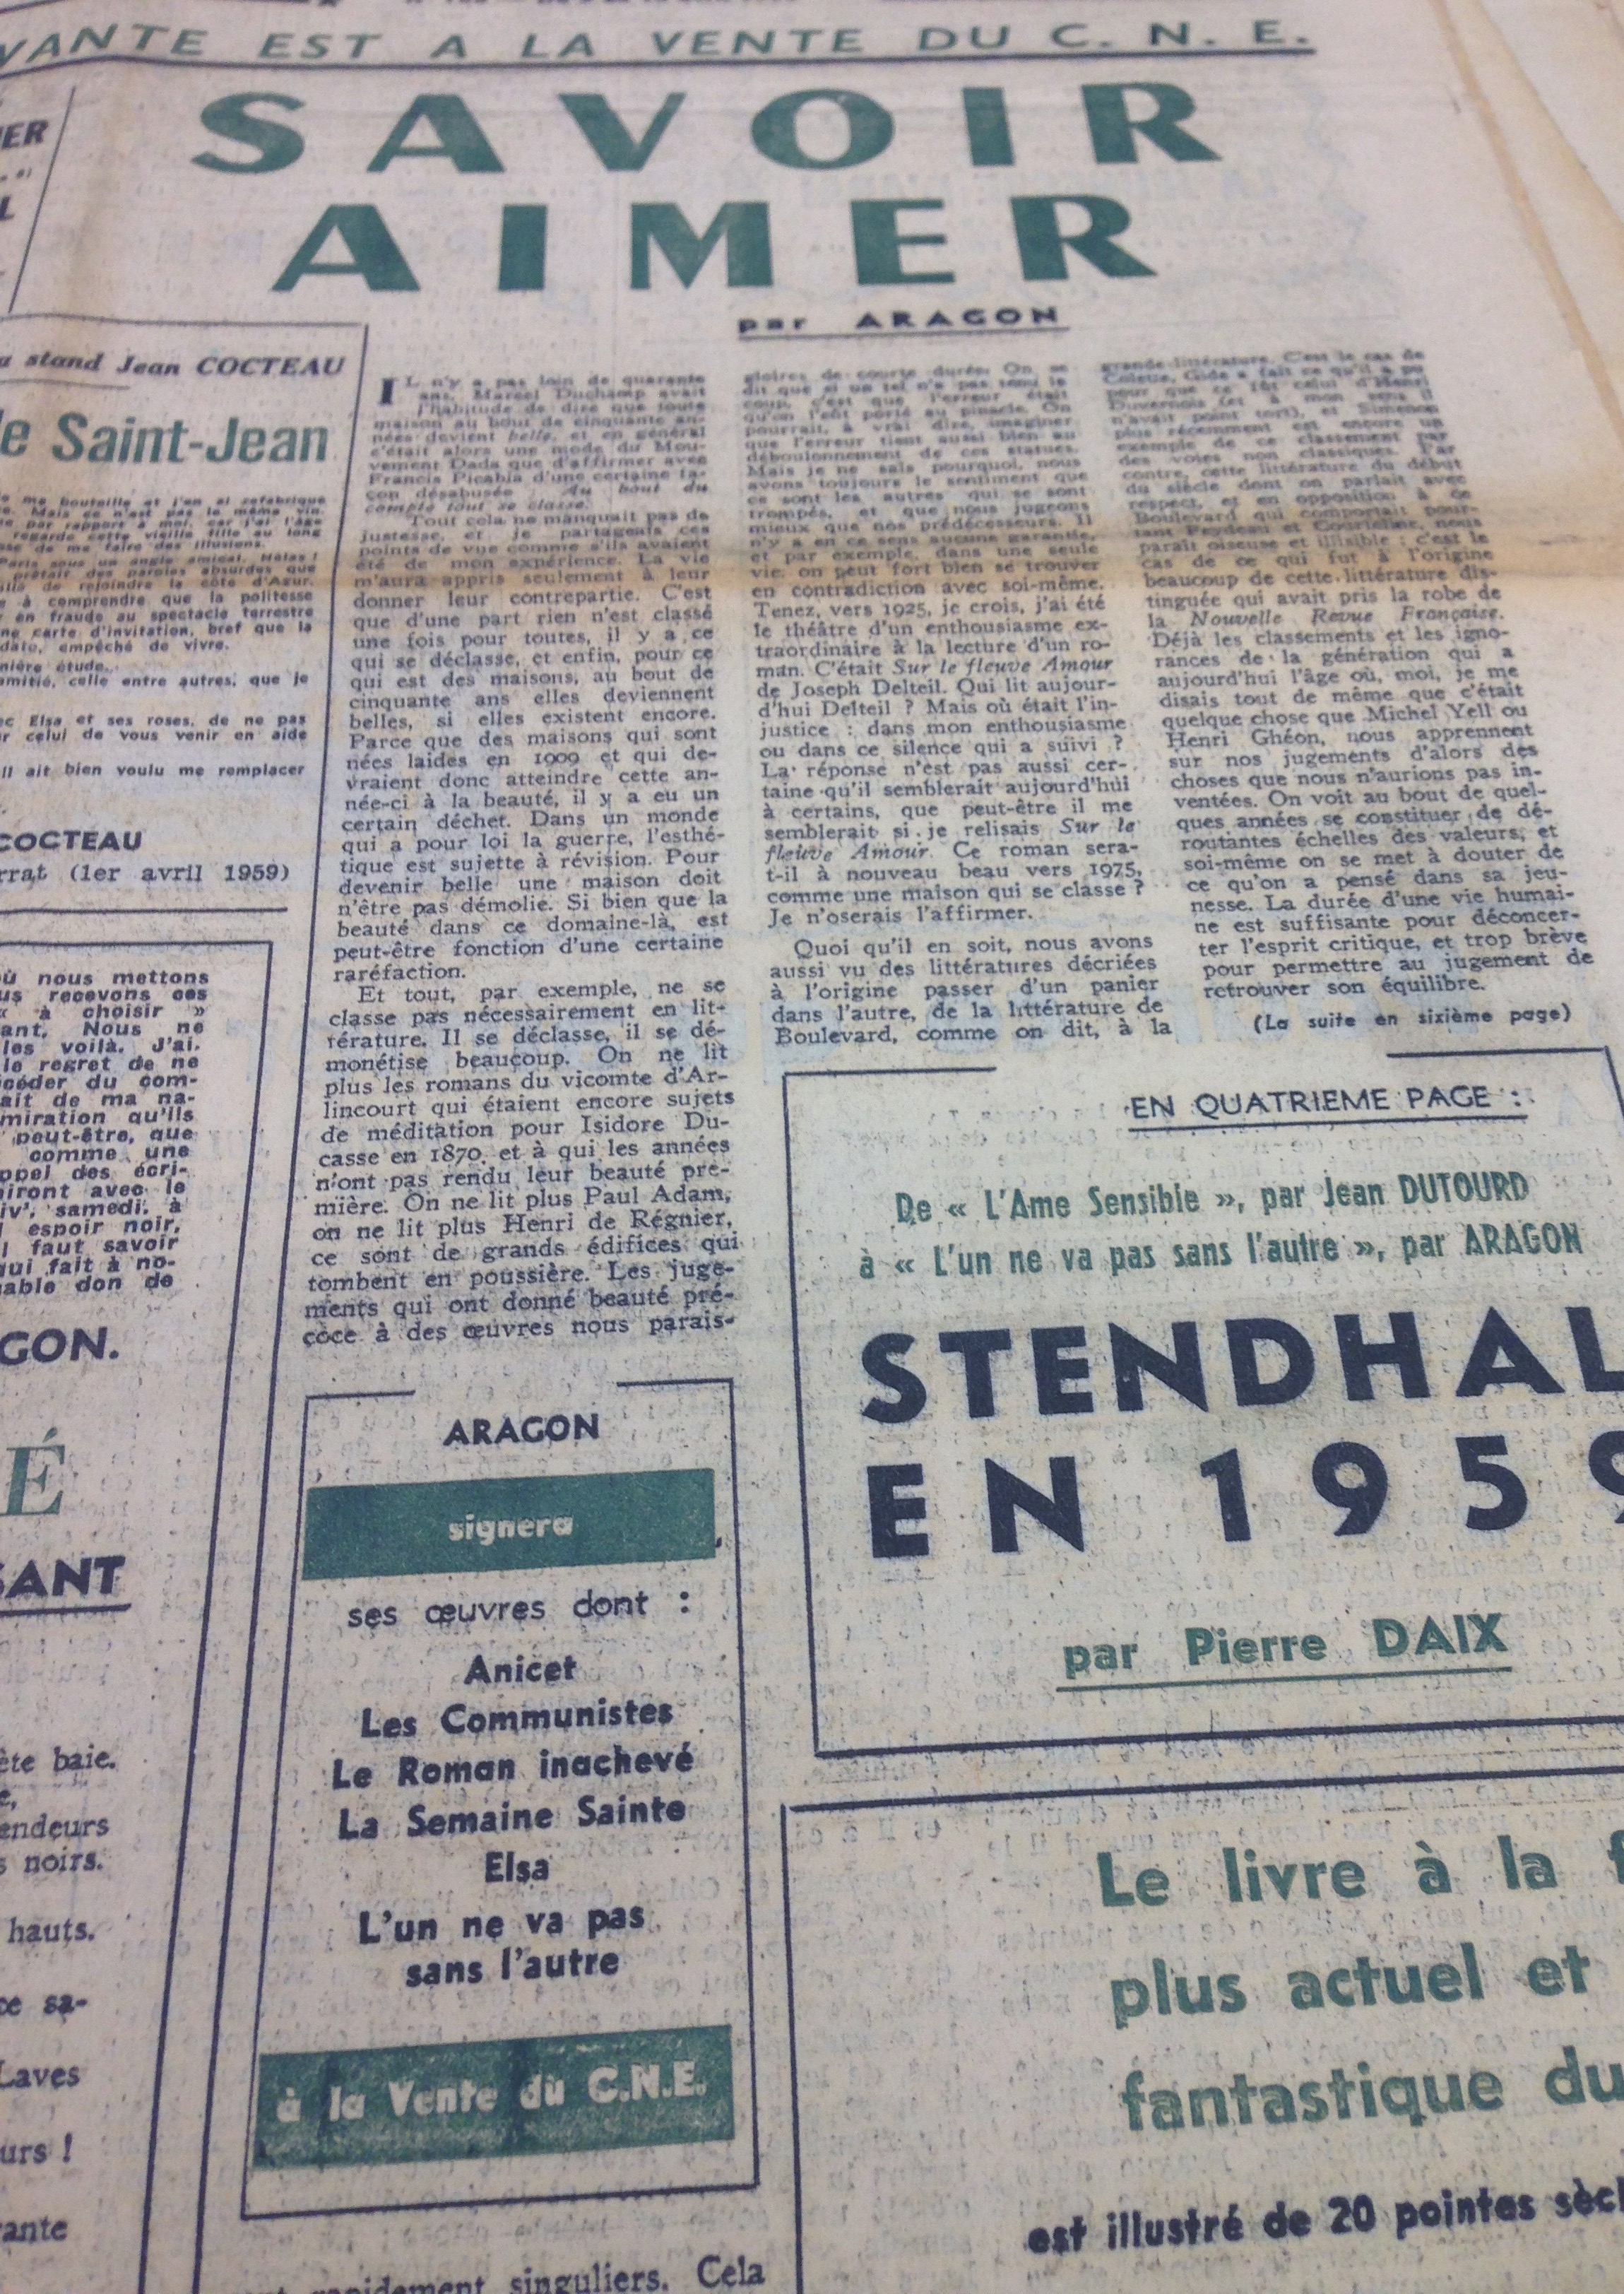
\includegraphics[width=0.75\textwidth]{savoiraimern708.jpg}
	\caption{\cite{savoiraimer}}\label{fig:Savoiraimer}
\end{figure}


Dans un troisième temps, à la lumière de la corrélation du travail esthétique et du message politique dans \emph{Les Lettres françaises}, il convient de mesurer le rôle de cet aspect du lyrisme révolutionnaire dans le traitement du réalisme socialiste. Cette notion dont Aragon se fait le grand représentant avec ses \oe{}uvres romanesques du \emph{Monde réel} en France vient de ses nombreuses lectures et voyages en URSS. L'\oe{}uvre littérature, comme les arts en général, se conçoit comme le miroir de la société du point de vue du prolétariat. L'évolution du réalisme socialiste dans \emph{Les Lettres françaises} est particulièrement retrace son succès jusqu'à sa tentative de sauvegarde révélateur lorsque Arago doit peu à peu y renoncer, surtout après 1956. Avec les révélations du Rapport de Khrouchtchev, le modèle de Staline désacralisé. Cependant, le réalisme socialiste, lui, met du temps à s’éteindre complètement, notamment dans les articles de critique d’Aragon. 

	 Aragon publie son article \emph{Savoir aimer}\footcite{savoiraimer} un an après une autre grande enquête, celle déjà évoquée de 1958 : \emph{Qu’est-ce que l’avant-garde en 1958 ?}\footcite{avantgarde}. Les influences du sujet sur cet article de 59 sont manifestes : Aragon semble répondre indirectement au sujet lorsqu’il revient sur son expérience dada : \enquote{c’était une mode du Mouvement Dada que d’affirmer avec Francis Picabia d’une certaine façon désabusée : \emph{Au bout du compte tout se classe}.}



 Mais un autre élément intervient pour évoquer ces \oe{}uvres hors-normes devenues académiques, celle de l’identité :  
 \begin{quote}
  Mais je ne sais pourquoi, nous avons toujours le sentiment que ce sont les autres qui se sont trompés, et que nous jugeons mieux que nos prédécesseurs. Il n’y a en ce sens aucune garantie, et par exemple, dans une seule vie, on peut fort bien se trouver en contradiction avec soi-même.\footcite{savoiraimer}\end{quote}

	Est-ce qu’on peut voir dans cette reconnaissance d’\oe{}vres contradictoires chez un même individu une possible mise à distance avec le réalisme socialiste ? Toujours est-il qu’à la fois en partant de ses convictions au temps de sa jeunesse et cette conception d’une identité altérée, Aragon semble revenir pourtant à son passé dada plutôt qu’il ne s’en éloigne. Cette logique d'association d'idées par  « classement » poursuit le procédé de ces mouvements artistiques, mais s'inscrit aussi dans la philosohphie de l'identité mouvante : \enquote{Et tout, par exemple, ne se classe pas nécessairement en littérature. Il se déclasse, il se démonétise beaucoup.}\footcite{savoiraimer}

Ce procédé du classement, face aux changements et aux revirements du  classement des \oe{}uvres, ce serait en somme une exploration de soi. Et, vis-à-vis des variations qui constituent un individu à travers les années,  Aragon suggère un vertige de l’identité, qui esr aussi finalité de la critique : 

\begin{quote}
 On voit au bout de quelques années se constituer de déroutantes échelles de valeurs, et soi-même on se met à douter de ce qu’on a pensé dans sa jeunesse. La durée d’une vie humaine est suffisante pour déconcerter l’esprit critique, et trop brève pour permettre au jugement de retrouver son équilibre.\footcite{savoiraimer}   
\end{quote}
 

	 On retrouve cette dimension fondamentale du temps, avec ses changements de perspectives depuis la jeunesse. L’entre-deux du temps ne peut aboutir qu’au vertige de la critique, et non au lieu commun de la critique qui se situerait plutôt dans la distanciation, le juste recul. Il peut paraitre paradoxal que l’article s’achève en éloge du réalisme socialiste, alors qu’à cette période Aragon commence à se tourner vers une autre conception du réalisme, qui n’est pas sans rappeler celui de Masson lorsqu’il peint ou dessine les hommes. Le verbe \emph{aimer} ,porté par le titre \emph{Savoir aimer},  plusieurs fois marqué par un italique de soulignement, se substitue par cette distinction typographique à « critiquer ». Savoir aimer, c’est savoir véritablement critiquer :  

     \begin{quote}
       Je pense, pour ma part, que le goût est une chose essentiellement positive. Que la critique devrait, en matière de littérature, être une sorte de pédagogie de l’enthousiasme. Qu’un vrai critique est celui qui apprend à \emph{aimer}, et attention ! j’emploie toujours verbe aimer au sens fort, j’entends ici que les critiques ne font pas leur métier, parce qu’on ne les voit jamais les yeux cernés pour avoir lu un livre, même quand ils en disent du bien.\footcite{atraversgaleries}    
     \end{quote}


	 Cette conception très lyrique de la critique, avec pour essence l’idée d’ \enquote{aimer}, est donc très proche de celle de Masson critique de Baudelaire comme critique dans l’article de 1968, neuf ans plus tard. Aragon et Masson partagent cette idée fondamentale d’une subjectivité du critique qui perdrait toute distance avec le sujet pour au contraire se plonger dans le vertige que procure l’\oe{}uvre. Comme chez Masson, pas seulement dans ses conceptions mais aussi dans son art, Aragon associe à cette exigence mentale une conséquence physique, due à l’obsession du critique sur le sujet, qui se répercuterait sur le système nerveux. Cet entrelacement de la pensée et du physique conduit logiquement à la métaphore de l’acte sexuel, : \enquote{Et personne ne songe à vous traiter d’impuissants, parce qu’on ne vous entend pas crier, quand vous lisez les romans ou les nouvelles de ce temps-ci. Il m’arrive de penser que c’est pour le moins étrange.}\footcite{savoiraimer} La métaphore est intéressante si l'on se rappelle que le l'érotisme valait comme symbole de liberté totale dans \emph{Le Con d'Irène}. 

     	Une révolution intérieure, comprise comme retournement des sens, doit envahir le critique, avec cette image insaisissable du cri. La même image du cri que Masson figure pour représenter la révolte paysanne. Comme Masson le revendiquera quelques années plus tard, Aragon encourage la passion que devrait susciter la critique, la prise de risques du jugement : \enquote{Bien parler d’un livre c’est peu. Il faut encore le situer. Oser dire, ceci restera}.\footcite{savoiraimer}

 Or, ce choix de déterminer ou pas la destinée d’une \oe{}uvre peut déjà se concevoir comme un choix politique. Celui d’anticiper, selon le jugement de valeur, une vision à long terme de l’\oe{}uvre sur le sens politique. Elle se confirme avec cette « envie partisane » selon l’expression d’Aragon qui implique le geste du choix, en  particulier ce rôle crucial du critique, celui qui peut décider si le sort d’une \oe{}uvre se prolonge dans le temps : 

\enquote{ce mécanisme indémontable de l’art, par quoi se fonde la grandeur de l’\oe{}uvre, et son droit à ne pas mourir}\footcite{savoiraimer} Le lyrisme de l’argumentation n’est pas seulement théorique, il est aussi typographique : Avec l’italique déjà abordé du verbe \enquote{aimer} qui insiste ainsi sur la force donnée au mot, mais aussi avec les majuscules, où  \enquote{J’AIME les choses bien faites} est redoublé quelques lignes plus tard par \enquote{JE ne sais pas comment vous avez la tête faite, et de quoi elle est peuplée : pour moi, j’ai toute la vie porté en moi des images dont rien ne pourrait me séparer.}\footcite{savoiraimer}

Le lyrisme est clairement manifesté avec ces majuscules autour du \enquote{je} et du verbe sur l’expression des sentiments par excellence. Sans compter que le sens de ces deux phrases éloignées dans l’article tournent autour de la même notion, même si la seconde phrase est plus explicite : le lyrisme vient des images qui hantent le critique. Ce qui rappelle le rapport aux images du processus de l'écriture et du dessin automatique, selon les critères surréalsites, dont la création émanait de ce débordement d'images incontrôlées. 

	Et pourtant, c’est encore par une sauvegarde du réalisme socialiste qu’Aragon ponctue finalement, comme le lieu même de l’amour : 
\begin{quote}
  l’amour pour que je le ressente, que je le partage doit  être réel, et réaliste l’art qui le décrit, et que c’est l’étrange calomnie que de prétendre que si ce réalisme a le socialisme pour soleil l’amour s’y doit étioler, quand c’est au contraire cet \emph{idéal qui donne à l’histoire réelle, la force même de l’amour}.\footcite{savoiraimer}\end{quote}


Pour aboutir au réalisme socialiste, Aragon soit revenu sur les autres formes de réalisme du temps de sa jeunesse. En 1959, le réalisme socialiste va peu à peu dans ses \oe{}uvres laisser la place à une autre perspective du réalisme. Néanmoins, cette conception de la critique rejoint à bien des égards sa position de critique de poésie dans les fameuses \emph{Chroniques du Bel Canto} de 1946 : 

\begin{quote}C’est un phénomène auquel il ne semble pas que les critiques se soient arrêtés : l’éclectisme nouveau et bizarre de la poésie des derniers temps…Comment ne pas voir qu’il reflète, que notre poésie écartelée reflète les incertitudes de esprits, l’égarement social, le trouble de l’homme ? La poésie est le miroir brouillé de notre société. Et chaque poète souffle sur ce miroir : son haleine différemment l’embue.\footcite[p93]{belcanto}\end{quote}

 Aragon se distingue d'une certaine pratique de la critique très distante de son sujet, et par opposition transforme le critique lui-même en poète. Le poète et le critique sont conciliés par la métaphore du miroir qui lie la poésie à l'idée d'actualité, puisqu'elle reflète l'état des esprits des hommes. Le lyrisme est ainsi déjà introduit comme une condition du travail de critique :

\begin{quote}Il nous faut prendre comme un fait le bariolage des techniques poétiques l’habit d’Arlequin des faiseurs de nuages. C’est un signe. Et qui traduit des phénomènes mal connus, en eux-mêmes difficilement saisissables. Comme l’ombre du passant,lyrique, amplifiée, trahit parfois sur les murs ses intimes incompréhensibles pensées cachées.\footcite[p94]{belcanto}\end{quote}

Le lyrisme est perçu comme un état de l'homme, de ses tumultes intérieurs. Ce \enquote{miroir du réel} du travail de critique projette cette particularité de l'homme sur son objet. Cette position de la transition entre l'après-guerre et la guerre froide poursuivie jusque dans l'article de 1959 \emph{Savoir aimer} revitalise par le lyrisme le réalisme socialiste à bout de souffle.


	Cet article revendique l’entrelacement du lyrisme et d'une dimension politique le fait sur deux aspects : d'une part, une notion subjective propre au choix, celui de faire perdurer une \oe{}uvre plutôt qu’une autre. Ce qui se rapproche d’une politique éditoriale dans les choix d’articles et la mise en page d’un numéro. En particulier pour le journal \emph{Les Lettres françaises}, qui, par sa position avant tout culturelle, est nourri en grande partie de critiques. C’est donc toute la ligne éditoriale du journal qui est explicitée dans l’article, son \enquote{envie partisane}et la recherche du vertige dans les agencements d’articles comme dans le choix des sujets. D’autre part, on peut concevoir cet article comme un entre-deux, ou plutôt un mouvement pris dans la réflexion d’Aragon à propos du réalisme socialiste : à la fois l’idée même du socialisme qui, chez Aragon, procure au lyrisme sa force subversive. Et, en même temps, des traces d’affinités pour une autre conception du réalisme font déjà pressentir les nouvelles réflexions romanesques en cours pour Aragon en tant qu’auteur. 

	

\subsection{Les échanges d'André Masson avec \emph{Les Lettres françaises }}

L’année 1959 semble être l’année de l’entre-deux, pour Aragon d’une part, mais pour Masson aussi, si l’on s’en tient à ses \oe{}uvres exposées au Salon de Mai\footcite{salondemai} en mai 1959 : \enquote{un André Masson plein de fougue qui illustre la transition entre le surréalisme et l’abstraction}, d’après Georges Boudaille. Un même mouvement de transition s’opère chez Aragon comme chez Masson, entre les élans de retours vers des affinités premières, et les prémices d’une réflexion autre qui émerge de cet entre-deux. Même si Boudaille qualifie de \enquote{fougue} la force des \oe{}uvres expressives de Masson, la toile représentée sur la page dans l’article, \emph{Un couple dans la nuit}, revient dans un autre numéro pour illustrer un texte de Claude Durand. Toujours sur ce thème de l’entre-deux, entre le jour et la nuit, où le lyrisme du personnage qui erre dans les rues la nuit et revit des discussions de couples se manifeste plus comme un écho à la réflexion du narrateur qu’à une illustration : 


\begin{quote}
Ivresse des limites perdues. Mais, parce que je suis seul, aucune épouvante ne me saisit (c’est ce qui nous ressemble qui nous terrifie). L’angoisse ? Ce vide m’était encore tout à l’heure mon droit à la joie, presque une plénitude…A quoi est-ce que je crois ?\footcite{durand} 	
\end{quote}
% Mettre illsutration "Un couple dans la nuit".


\begin{figure}[H]
   \centering
   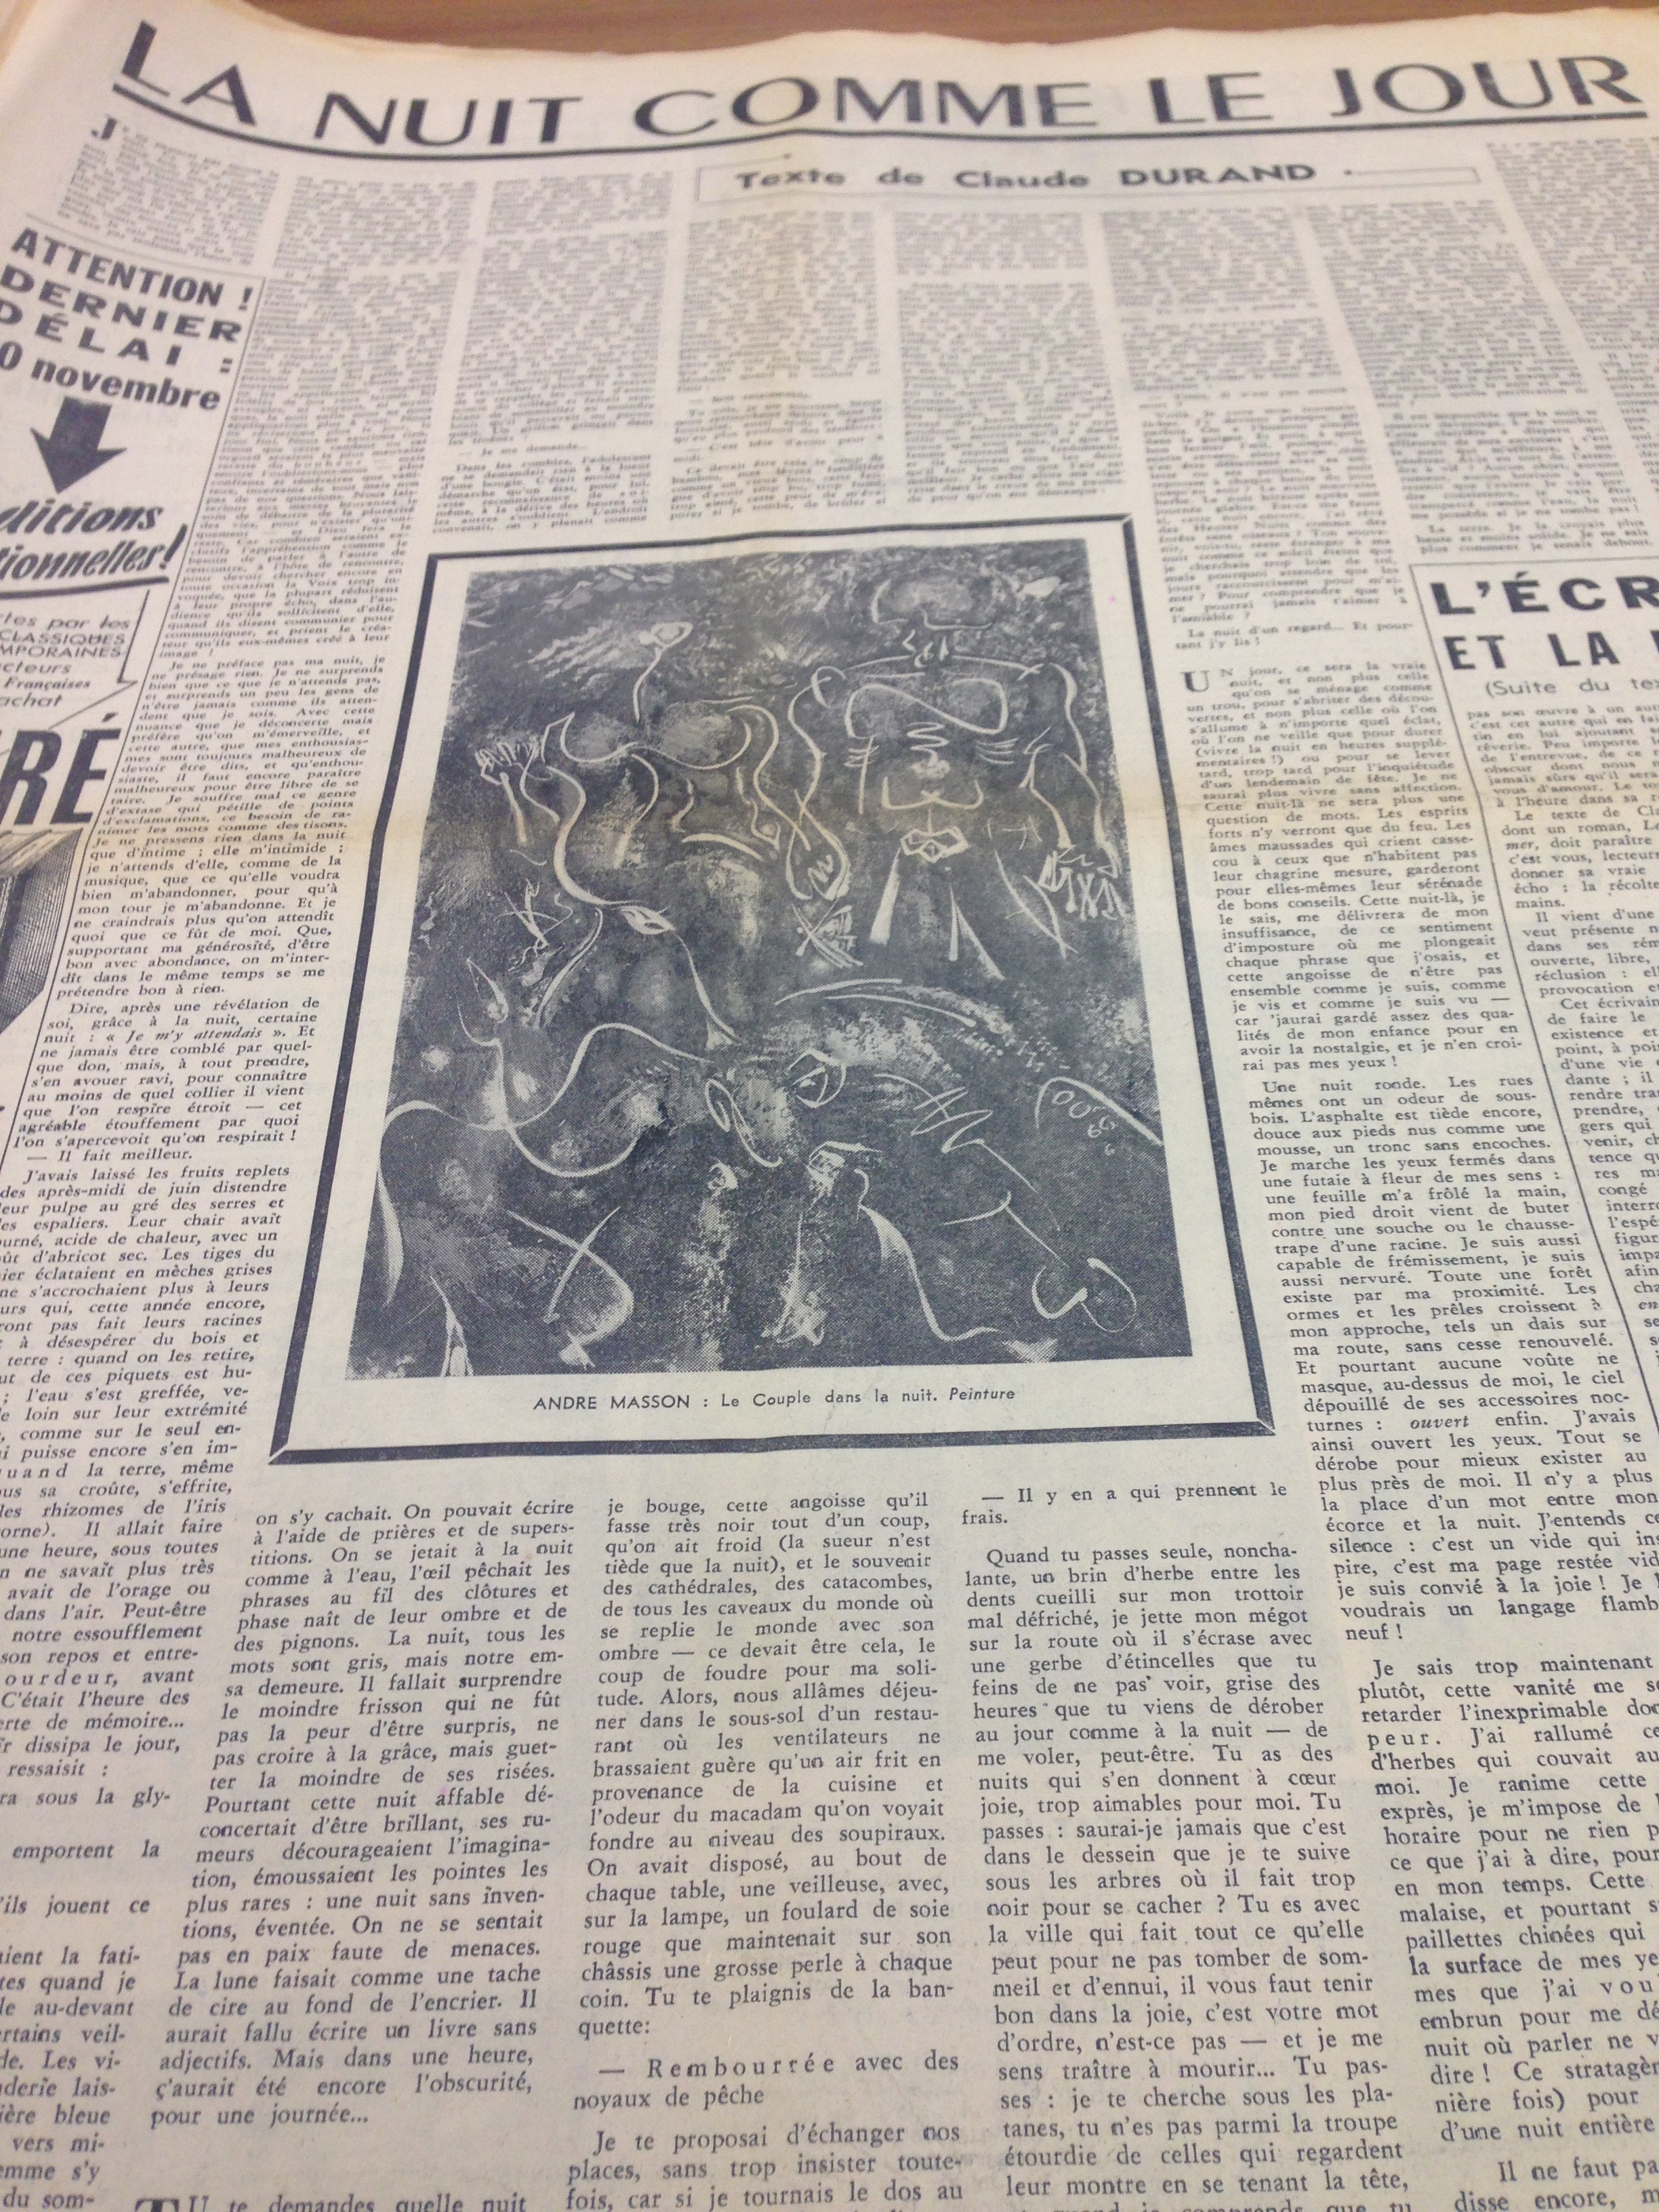
\includegraphics[width=0.75\textwidth]{couplenuit.jpg}
	\caption{\cite{durand}}\label{fig:Un couple dans la nuit}
\end{figure}


 Or, l’angoisse, plus qu’un sentiment, est un véritable moyen d’expression dans l’art d’André Masson. Dans l’article de Georges Boudaille comme dans le texte de Claude Durand, le titre de l’\oe{}uvre de Masson apparemment serein est ainsi qualifié par l’énergie et l’errance, thème romantique. Il est vrai que, si les silhouettes de l’homme et de la femme sont immédiatement perceptibles, c’est par leurs traits appuyés plutôt que par la représentation d’une chair. Leur main entrelacée, par un croisement de lignes, n’en figure qu’une seule. Paradoxalement, les lignes apportent l’érotisme à leur corps nu, de façon plus directe que s’il s’était agit d’une représentation réaliste et fidèle d’un homme et d’une femme. La force symbolique que procure les lignes pour former les corps nus rapprochent ce couple plus d’une Idée au sens symbolique, plutôt que de personnages, chargés de jouer un rôle quelconque dans l’\oe{}uvre.  


De plus, Pierre Descargues qualifie l’esthétique d’André Masson de \enquote{réel fantastique} dans son article \emph{André Masson et le réel fantastique}\footcite{reelfantastique}. Aragon venait de  prendre l'année précédente la direction  de la rubrique \emph{Tous les arts}. Pierre Descargues y occupe conjointement avec Aragon une chronique, \emph{A travers les galeries}. Ainsi, tout comme d’autres chroniqueurs tels que Georges Boudaille ou Georges Besson, Descargues connaît intimement Aragon et André Masson. 

\begin{figure}[H]
   \centering
   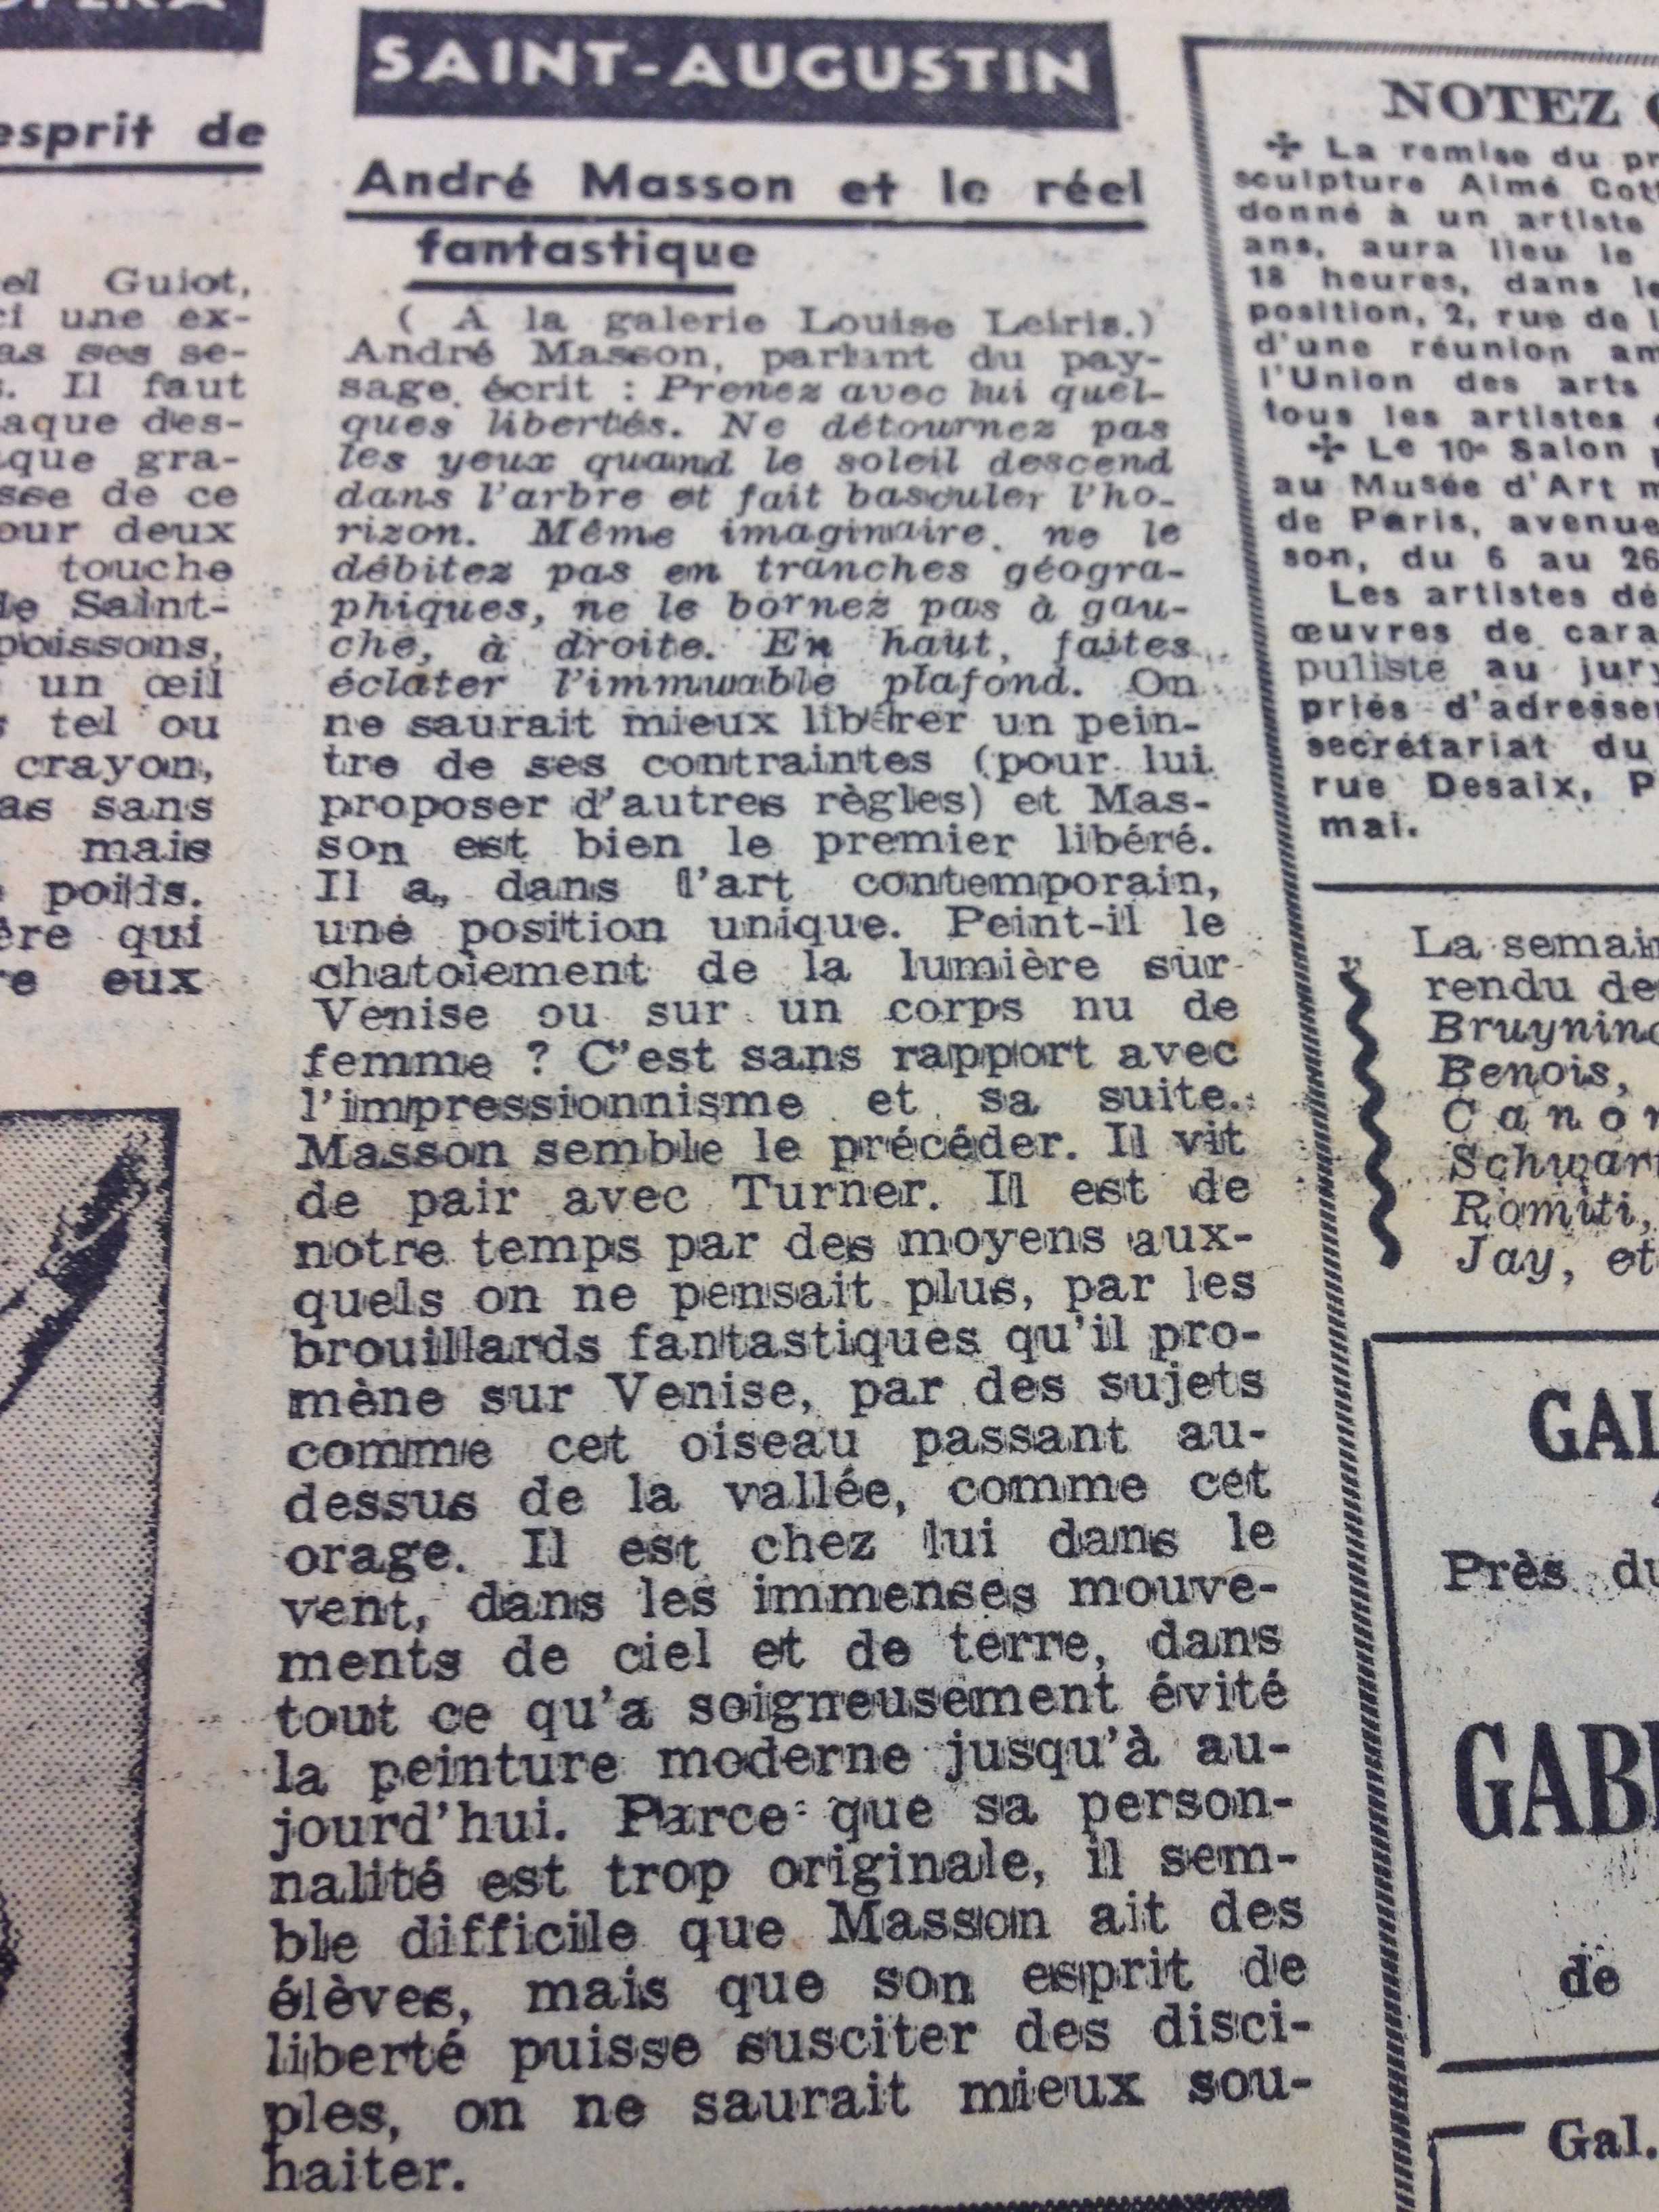
\includegraphics[width=0.75\textwidth]{textereelfantastiquen411.jpg}
	\caption{\cite{reelfantastique}}\label{fig:Articlereelfantastique}
\end{figure}

\begin{figure}[H]
   \centering
   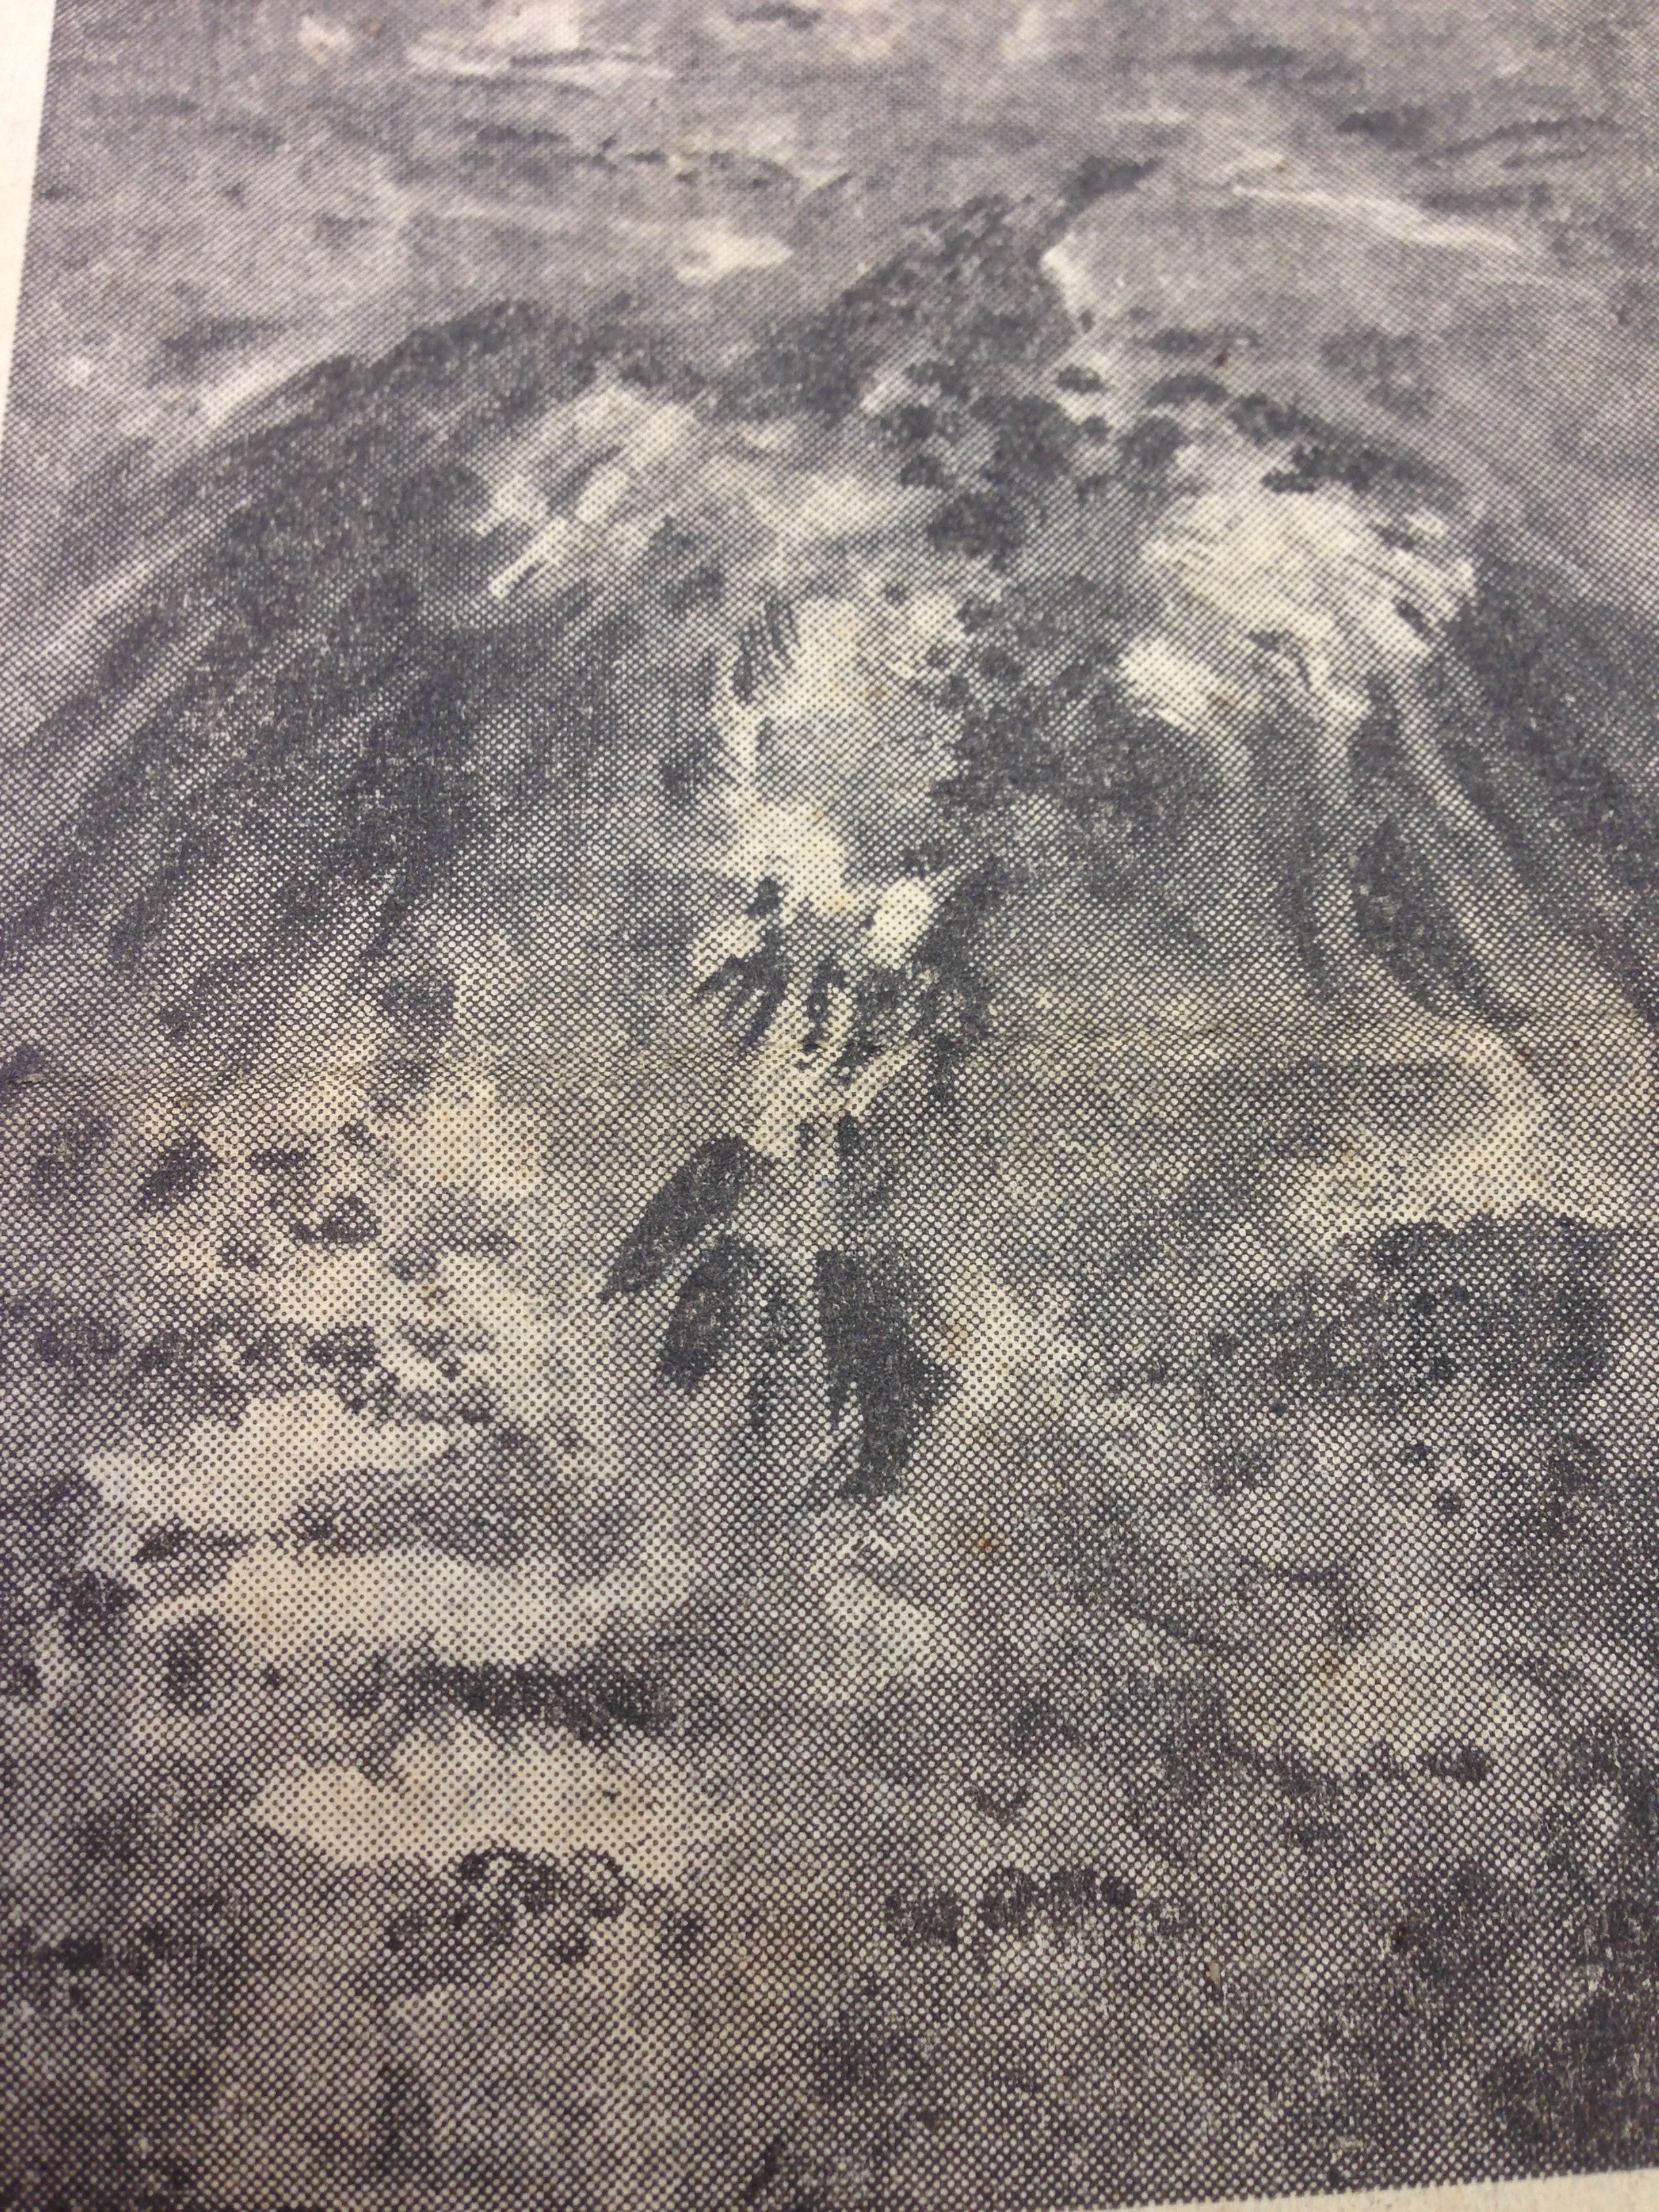
\includegraphics[width=0.75\textwidth]{reelfantastiquen411.jpg}
	\caption{\cite{reelfantastique}}\label{fig:Imagereelfantastique}
\end{figure}


	Il s'avère que, au début des années 50, la politique éditoriale est toujours tournée vers une politique de paix dans un contexte de guerre froide, avec le symbole des colombes massivement représenté depuis 1948, et la défense du réalisme socialiste. Est-il possible que cette page de la rubrique des Arts propose implicitement un croisement entre le réalisme socialiste et le réel fantastique ? En ouvrant son article avec des mots de Masson à propos de l’art de figurer le paysage, c’est le lien étroit entre le réel et l’imaginaire qui est pointé : 

 \begin{quote}
Prenez avec lui quelques libertés. Ne détournez pas les yeux quand le soleil descend dans l’arbre et fait basculer l’horizon. Même imaginaire, ne le débitez pas en tranches géographiques, ne le bornez pas à gauche, à droite. En haut, faites éclater l’immuable plafond.\footcite{reelfantastique}\end{quote}

	 En somme, selon Descargues, Masson revendique le contraire de l’ordre. Non seulement il préconise à l’artiste des \enquote{libertés}, mais la Nature elle-même comporte une part subversive pour lui. Ce qui explique le geste de l’artiste subversif aussi pour Masson qui ne recherche pas la mimétique de la Nature,refuse l'ordre classique et aligné de la composition, pour au contraire \enquote{éclater l’immuable plafond}.

	  Cette idée de jaillissement rappelle même plus l’abstraction que la figuration, à ceci près qu’une fois encore il s’agit de se détourner du mimétique pour l’expression de la Nature, et son éventuel réalisme véritable. Or, ce réalisme ne peut être possible qu’avec ce facteur fantastique, ce qui selon Descargues est plutôt tourné vers l’idée de l’imaginaire et de l’onirique. On relève donc la dimension paradoxale d’un réalisme qui advient par l’imaginaire et le rêve dans le but de figurer l’essence de la Nature, ce qu’elle veut signifier, plutôt que sa copie. C’est qui fait écrire au critique que Masson est en somme un insaisissable : 
 
En outre, l’allusion à Turner est d’autant plus parlante pour les quelques lignes que Masson lui avait sacré au début de cette même année 1952 (clin d’\oe{}il de Descargues ? ) : \enquote{Disparition de la pesanteur}. Ces propos sur Turner sont essentiels pour comprendre qu’en refusant le mimétique, Masson a aussi délibérément choisi de de composer avec des lignes plutôt qu’avec l’effet de masse. La forme faite de lignes fait deviner plus qu’il ne le signifie directement, puisque le sujet est dépossédé de sa masse corporelle. Sans compter qu’on peut considérer Turner comme faisant de l’impressionniste avant l’heure, ce qui fait de son mouvement aux couleurs chaudes un art insaisissable à son époque d’une façon similaire à André Masson. 

Il  s’agit de constater comment le \enquote{réel fantastique} de Masson  croise le projet du réalisme socialiste qui est celui de la politique éditoriale. Sa part de romantisme révolutionnaire est étroitement liée au réalisme socialiste. 


	Reynald Lahanque offre une première piste sur les motivations éditoriales du journal, et plus précisément d’Aragon comme responsable de cette rubrique Tous les Arts, quelques mois avant d’être officiellement directeur de tout l’hebdomadaire, dans sa thèse sur le réalisme socialiste en France : 

\begin{quote}
Le terme même de \enquote{réalisme socialiste}se rencontre assez rarement dans \emph{Les Lettres françaises}, mais la problématique que le terme recouvre y est très largement présente. Dirigé dans les faits par Aragon et Daix, l'hebdomadaire culturel fait toute sa place, sur un plan plus général, aux thèses et aux thèmes de la propagande communiste de la guerre froide. Il garde en même temps l'ambition de toucher un public plus large que celui des militants, et conserve des collaborateurs moins engagés politiquement et capables d'élargir la gamme de ses centres d’intérêt. \footcite{}\end{quote}

	Comme pour toute politique, le choix éditorial met en valeur un élément au détriment d’un autre. A dessein de ne pas se limiter à un lectorat proche l’appareil du PCF, le terme « réalisme socialiste » subit un profond paradoxe : Il est plus que jamais à l’ordre du jour dans ce contexte de guerre froide, tout en restant discret en raison de sa connotation immédiatement politique. On retrouve ici ce qu’Aragon revendique quelques années plus tard en 59 comme l’\enquote{envie partisane}\footcite{savoiraimer}, essence du travail de critique. 

	\begin{figure}[H]
   \centering
   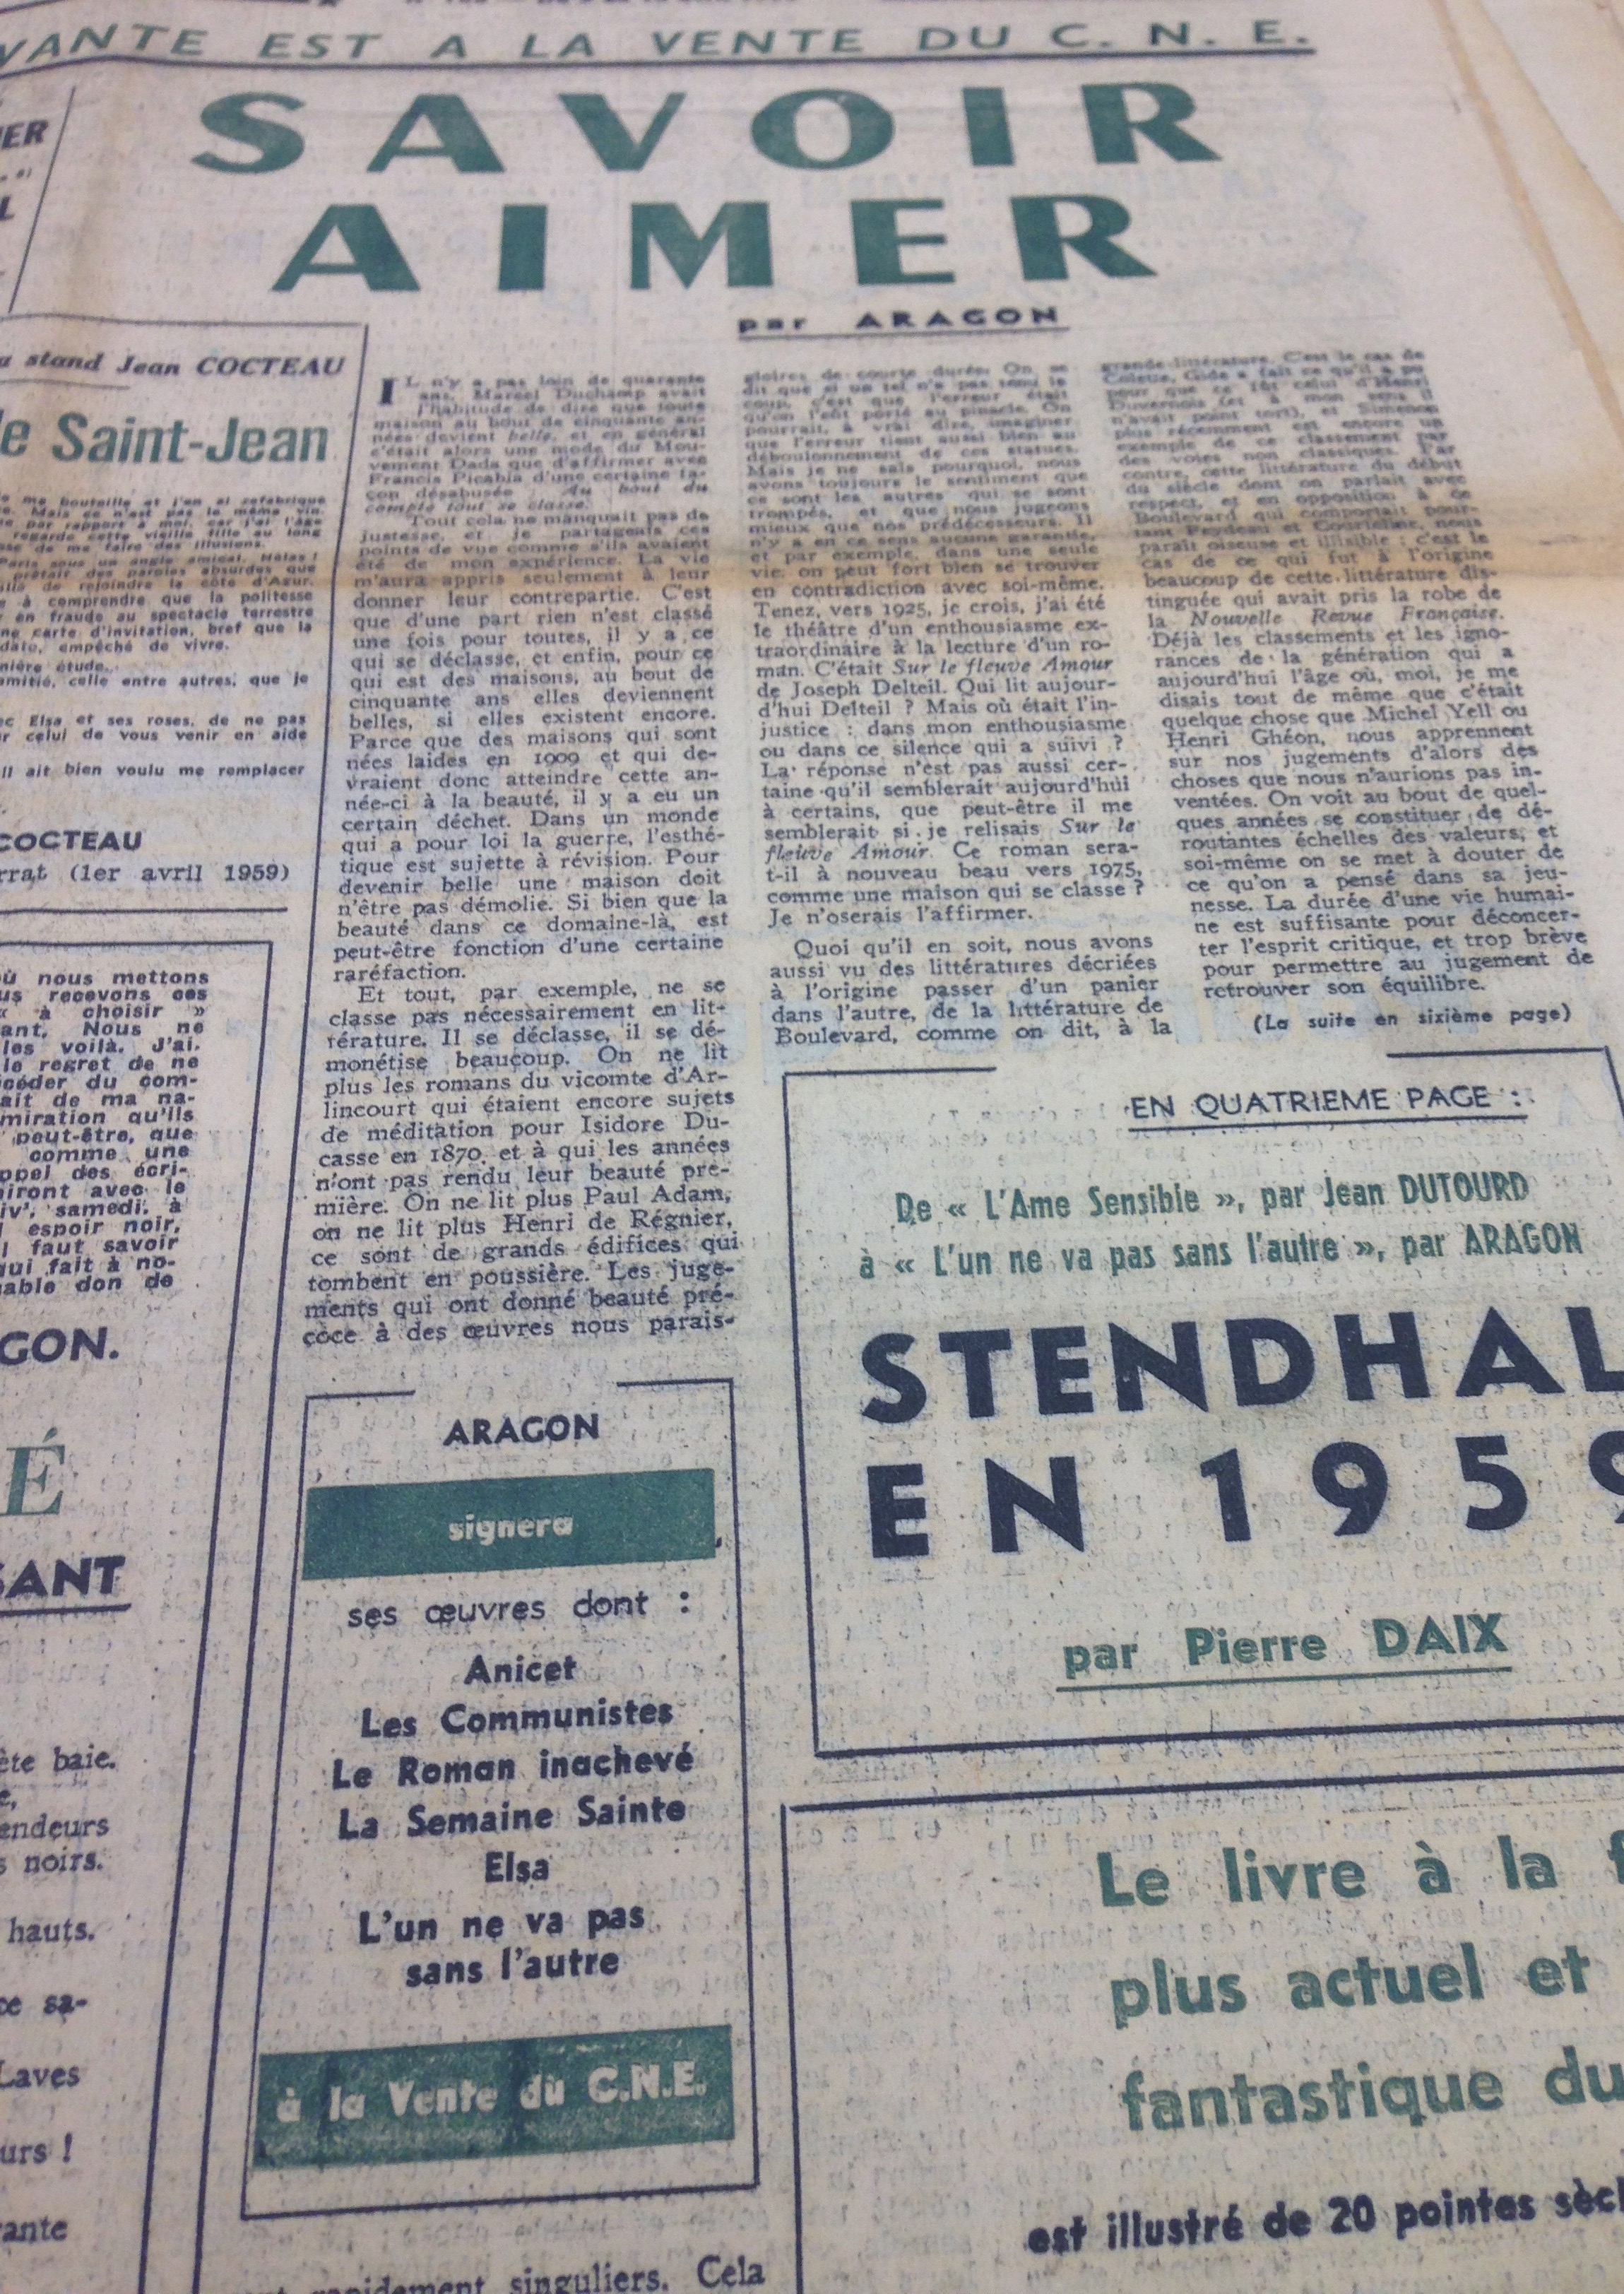
\includegraphics[width=0.75\textwidth]{savoiraimern708.jpg}
	\caption{\cite{savoiraimer}}\label{fig:Savoiraimer}
\end{figure}


Si l’\enquote{envie partisane} existe déjà en 1952, elle ne doit pas paraître invasive, puisqu’elle définit une idéologie précise en contradiction avec la politique éditoriale d’ouverture à un plus large public. Face à cette contradiction entre les attentes politiques et les attentes éditoriales, le mot d’ordre qui vient à la place envahir le journal, mais qui sous-tendrait au réalisme socialiste, c’est le mot \enquote{Paix}, omniprésent depuis les années 48, et d’une portée large, voire unanime.À peine quelques années après la Seconde Guerre Mondiale, qui voudrait encore la guerre ? Mais, sur le plan artistique, le \enquote{réel fantastique} pour désigner l’art d’André Masson pourrait lui-même aboutir idéologiquement à une forme dérivée du réalisme socialiste. Avec, cependant, une qualification onirique de ce réalisme qui n’apparente pas l’expression directement à une théorie politique. 

Jusqu’à son terme, la dimension proprement lyrique de l’article de Descargues, avec cette métaphore du vent qui incarne à la fois les représentations et la méthode de Masson, semble appuyer la rêverie et s’éloigner de tout aspect politique : \enquote{Il est allé chez lui dans le vent, dans les immenses mouvements de ciel et de la terre, dans tout ce qu’à soigneusement évité la peinture moderne jusqu’à aujourd’hui. Parce que sa personnalité est trop originale.}\footcite{atraversgaleries} On est apparemment plus proche des \emph{Rêveries d’un promeneur solitaire} de Rousseau que du réalisme socialiste. 

	Cependant, la liberté est aussi un concept politique fondamental, et c’est bien celle-ci qu’aspire à faire rêver au lecteur le mouvement lyrique. L’adverbe \enquote{trop} pour conclure sur la dimension atypique de Masson ne peut pas être anodine. En substance, l’art d’André Masson est un débordement. Peut-on alors supposer que le \enquote{réel fantastique} est un mode de représentation du réalisme socialiste ? La question peut trouver des réponses contradictoires, dans cette année 1952, où, dans un article d’éloge à la remise du Prix Staline au roman \emph{Le Premier choc} d'André Stil\footcite{prixstaline}, Aragon rappelle, non sans apparenter cette définition en partie à Staline, ce qu’est le réalisme socialiste : 
	\begin{quote}
	Le réalisme socialiste, étant la méthode de base de la littérature et de la critique soviétique, exige de l’artiste une représentation véridique, historiquement concrète de la réalité dans son développement révolutionnaire. De plus, le caractère véritable et historiquement concret de cette représentation artistique de la réalité doit se combiner avec le devoir de transformation idéologique et d’éducation des masses dans l’esprit du socialisme.\footcite{prixstaline}\end{quote}
	
	 Une telle définition demanderait à se poursuivre par la définition cette fois du socialisme. Est-il d’ailleurs le même en URSS qu’en France, si on prend en compte le fait que la politique du parti communiste diffère sur certaines caractéristiques d’un pays à l’autre ? Reynald Lahanque pointe d’ailleurs la pratique du réalisme socialiste d’Aragon dans les romans du \emph{Monde réel}. Il les juge peu représentatifs des héros communistes-types du réalisme socialiste et de scénario d’apprentissage grâce au Part. Mais, vis-à-vis du \enquote{réel fantastique}, ce qui est en jeu,c’est la question de la représentation \enquote{véridique, historique, concrète de la réalité} telle que l'exige le réalisme socialiste. 

 Cet appel à la figuration manifeste et plutôt naturaliste contraste donc avec l’aspect \enquote{fantastique} de Masson. Cependant, si l’on s’arrête aux louanges d’Aragon sur \emph{Le Premier choc}, l’aspect très pragmatique établi dans cette définition du réalisme socialiste est substitué à une autre forme de réalisme : \enquote{Je veux parler de sa façon de décrire les personnages. Ou plutôt de ne pas les décrire}.\footcite{prixstaline} On commence par cette suggestion d’une autre forme \enquote{concrète} du réel qui ne serait pas une forme naturaliste à se rapprocher de la conception d’André Masson sur la représentation des paysages. Ce constat sur lequel s’appuie Aragon repose sur un fondement analogue au « réel fantastique » de l’artiste de Descargues : il s'agit de figurer non le sujet en tant que tel, mais ce qu’exprime le sujet : \enquote{Parce que justement, ici, la ressemblance ne tient  pas à un \emph{trait} qui se répète. Mais à la nature complexe de l’homme décrit.} Cette phrase sur l’\oe{}uvre de Stil pourrait se confondre avec celles de Masson : le peintre revendique une idéologie esthétique contre le sujet figé du mimétique, et manifeste sa recherche de l’essence du sujet, sa nature. 


	Un tel projet ne peut que reposer en partie sur l’imagination comme moyen de représentation. Ce qu’Aragon dans ce même article nomme le \enquote{typage d’âme} : \enquote{Les personnages du \emph{Premier Choc} sont socialement définis et individuellement distingués par ce que j’appellerai le \emph{typage d’âme}. C’est à leur façon de penser, c’est au contenu de leur pensée, socialement définie- et au caractère de chacun, que l’auteur a fait appel pour fixer leurs images.}. Cette analogie entre \emph{Le premier choc} de Stil et l’\oe{}uvre d’André Masson illustre la conviction d’Aragon au début de l’article qu’avec le réalisme socialiste, on peut parler de la littérature pour évoquer l’art, et réciproquement.  Le choix stylistique de Stil est d’ailleurs bien plus qu’un détail pour Aragon, et peut-être est-ce même l’un des fondements qui permet à cette notion son \enquote{ développement révolutionnaire} comme finalité, d’après sa définition : \enquote{“Ce qui se passe dans leurs yeux est plus important que leur couleur“…Je vous dis que cette page que j’ai recopiée a valeur de manifeste.} La fonction poétique de la phrase n’est pas anodine, c’est même elle qui lui confère une forme de maxime. Le \enquote{typage d’âme} pourrait donc être le fil directeur à la fois du réalisme socialiste et des convictions d’André Masson. Dès lors, la notion de concret est complètement redessinée. Cependant, si une nature révolutionnaire associée à une forme lyrique est commune à la fois à l’article d’Aragon sur Stil et au réel fantastique de Masson, on peut distinguer cette finalité révolutionnaire : le réalisme socialiste comporte dans la suite de sa définition une valeur éducative, qui est peut-être l’élément que l’on ne retrouve pas de façon évidente dans le \emph{Monde réel}. André Masson réclame qu'on fasse \enquote{éclater l’immuable plafond}, mais pas à dessein nécessairement éducatif, tout au contraire. Dans l’exemple du paysage, celui-ci a la forme du fameux que l’on retrouve symbolisé dans beaucoup de ses \oe{}uvres, et cette expression du mouvement est une finalité en soi. La rationalisation du mouvement ne semble ni attendue ni souhaitée. 

Or, la définition du réalisme socialiste dans cet article d’Aragon pourrait comporter le paradoxe de sa finalité : \enquote{Le développement révolutionnaire} pourrait se concilier avec la seconde partie de la définition, \enquote{se combiner avec le devoir de transformation idéologique et d’éducation des masses dans l’esprit du socialisme.} Si le mouvement révolutionnaire comporte en substance une notion de liberté, rattachée par André Masson dans l’article sur le réel fantastique et à son art en général, celui-ci semble difficilement rentrer dans la finalité de contrôle et d’ordre que sous-entend \enquote{l’éducation des masses}. C’est pourquoi, tout en rappelant lui-même cette définition et l’influence de Staline, si l’on évoque les \oe{}uvres du \emph{Monde réel}, on peut se demander si les \oe{}uvres réalistes socialistes d’Aragon n’ont pas elles-mêmes tant recherchées \enquote{l’éducation des masses} que le \enquote{développement révolutionnaire} des personnages. 

\subsection{Comparaison des articles \emph{ Réalisme socialiste pas mort}d' Aragon \emph{A travers les galeries} de Pierre Descargues}

	Croiser un article de critique littéraire et un autre sur les expositions dans les galeries d’art en 1957 met en valeur la grande influence de la foi communiste du directeur du journal, Aragon, cette année-là. Les livres vont êtres analysés, comme l’indique très clairement Aragon dans son titre \emph{Réalisme socialiste pas mort}\footcite{realsoc}, son commentaire sur les livres \enquote{L’Homme ne vit pas seulement de pain}, de Vladimir Doudintsev, et de \emph{L’Or} de Boris Polevoï se fait dans l’éclairage du réalisme socialiste. Ce qui n’est pas anodin : Les \oe{}uvres sont louées pour leur valeur réaliste socialiste. 

\begin{figure}[H]
   \centering
   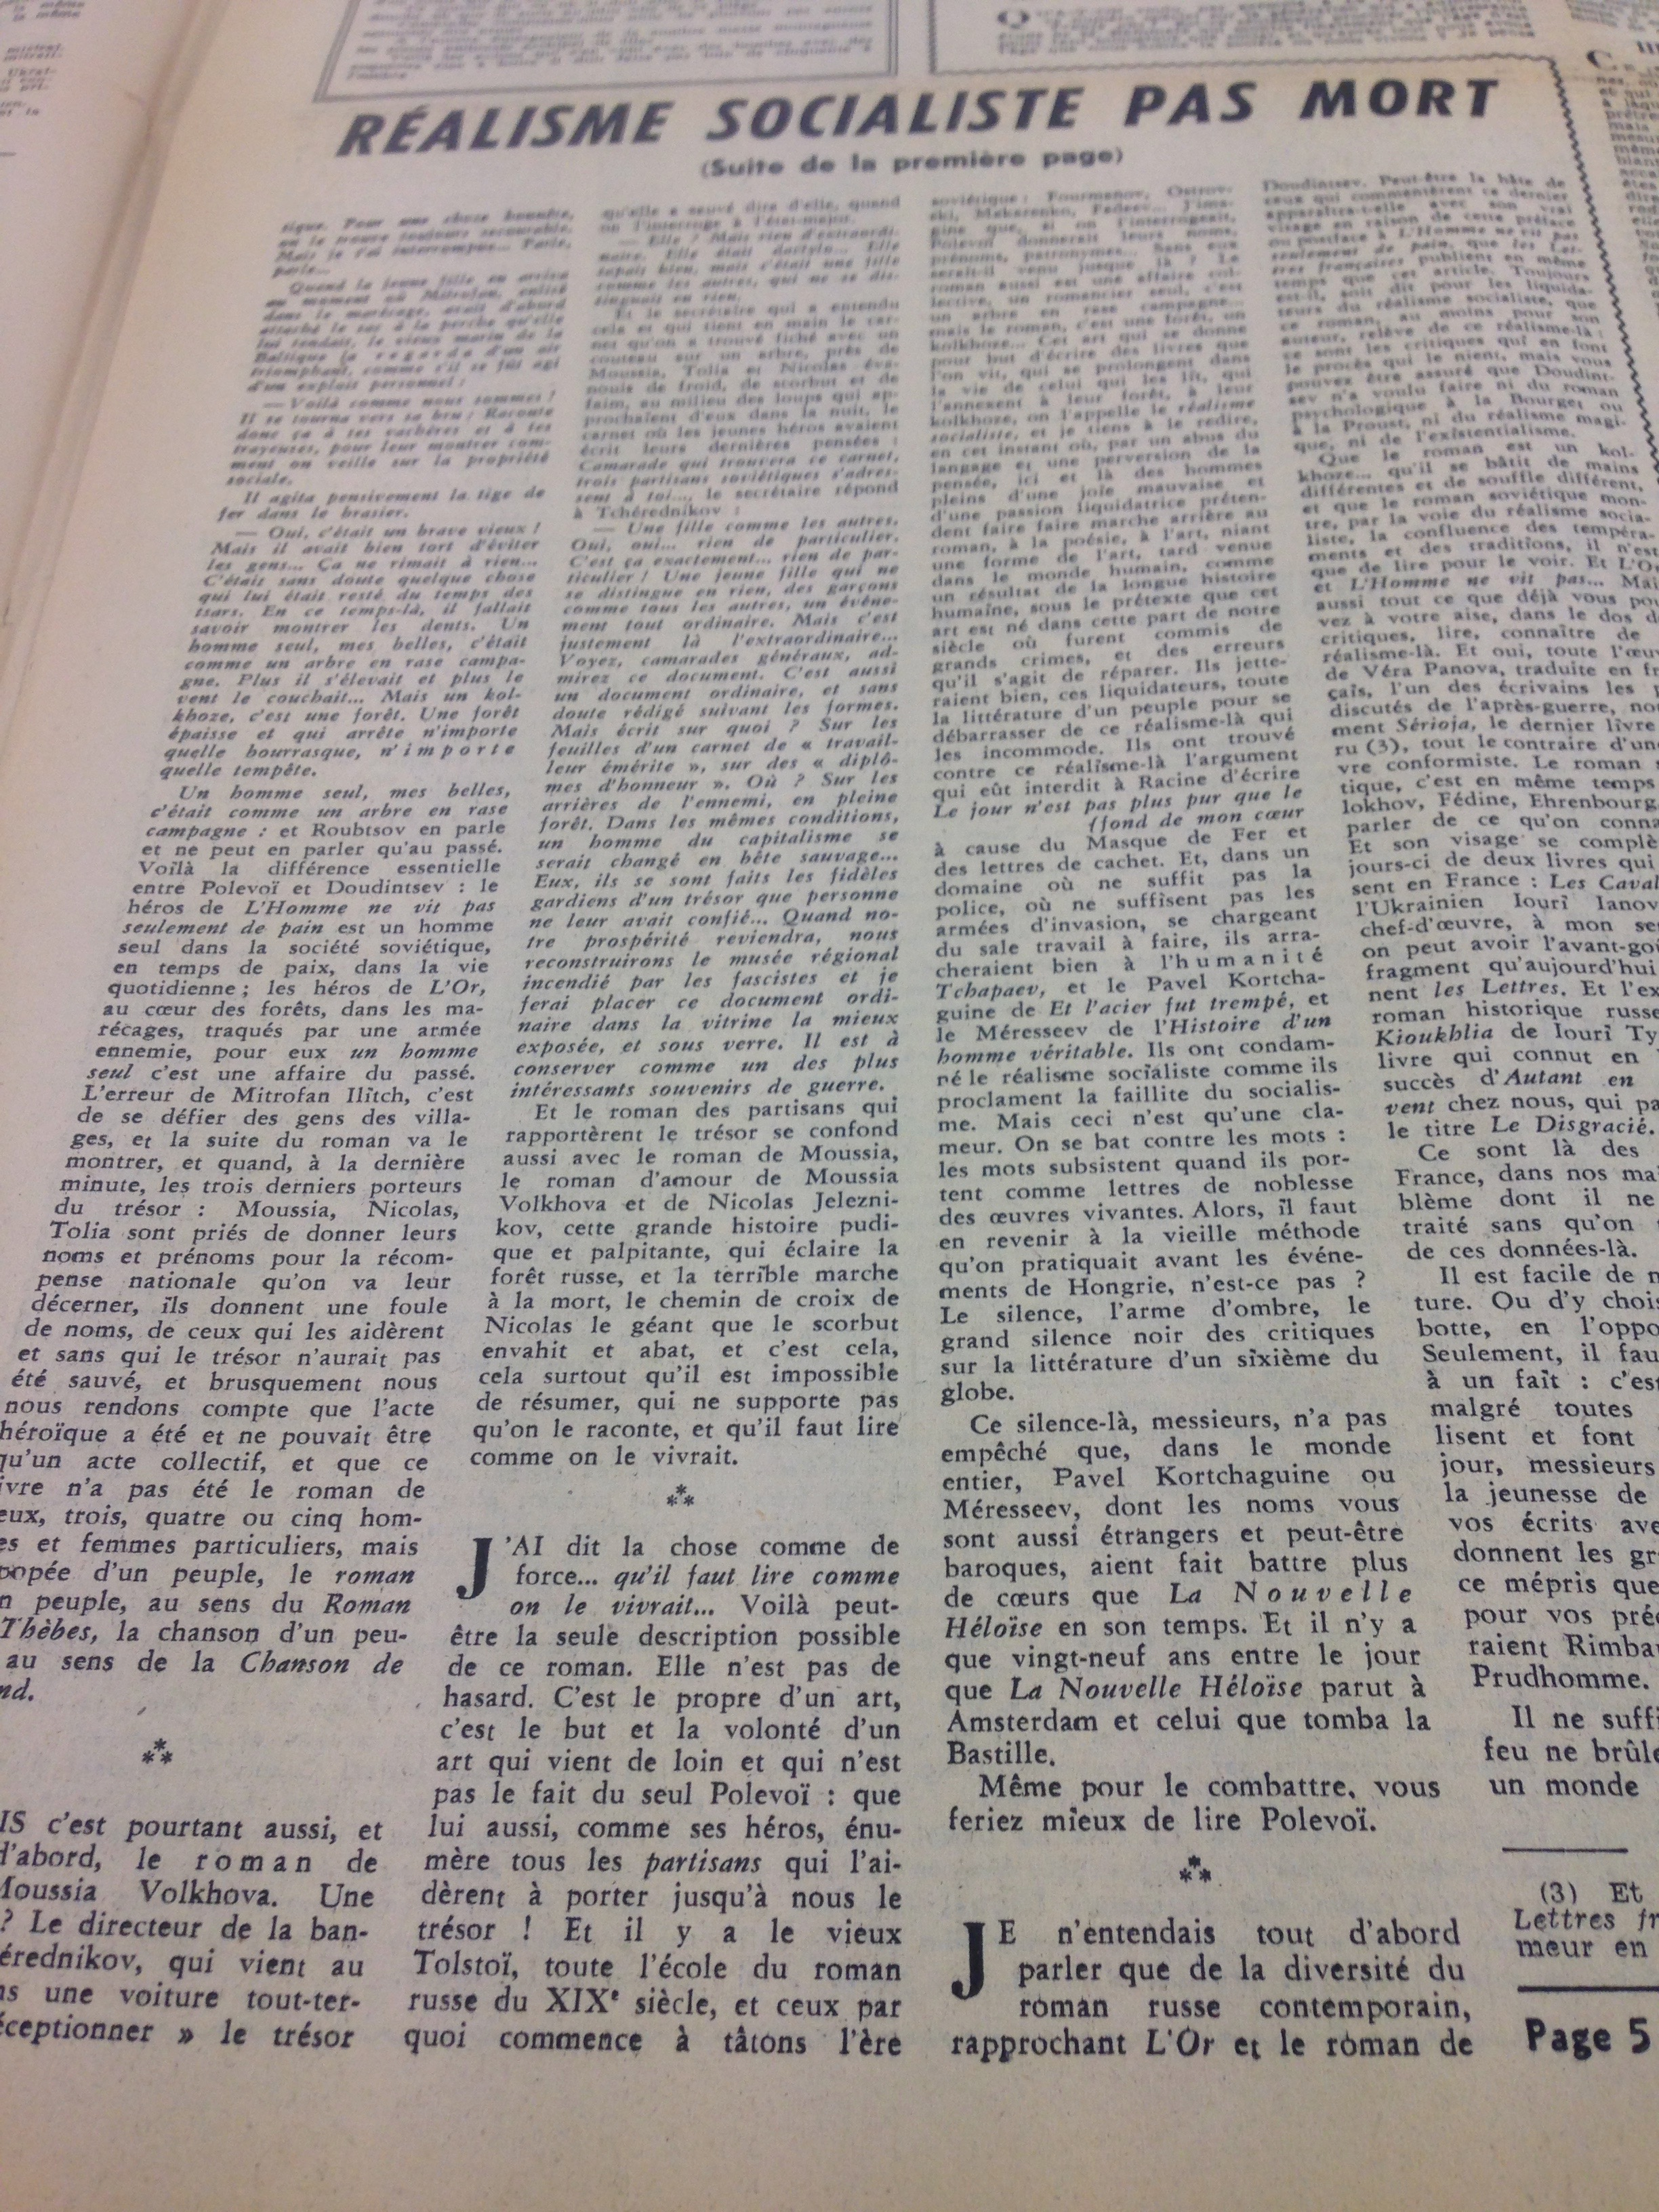
\includegraphics[width=0.75\textwidth]{realismesocialisten673.jpg}
	\caption{\cite{realsoc}}\label{fig:Réalistesocialistepasmort}
\end{figure}

	

	Or, comme dans beaucoup d’illustrations des \emph{Lettres françaises }lorsqu’il s’agit d’André Masson, c’est un dessin qui représente ses \oe{}uvres dans un numéro quelques mois plus tôt dans la rubrique \emph{A travers les galeries}\footcite{atraversgaleries}, par Pierre Descargues, illustré d'un Un dessin inachevé. On rejoint là encore, sur le plan artistique cette fois, une conception de la figuration étroitement liée à la politique communiste, et sur laquelle le réalisme socialiste peut en partie exercer une influence : celle de la préférence du dessin sur la peinture à l’huile. D’autant plus du dessin inachevé, plus proche encore de la genèse de l’\oe{}uvre et du geste originel de l’artiste. 

\begin{figure}[H]
   \centering
   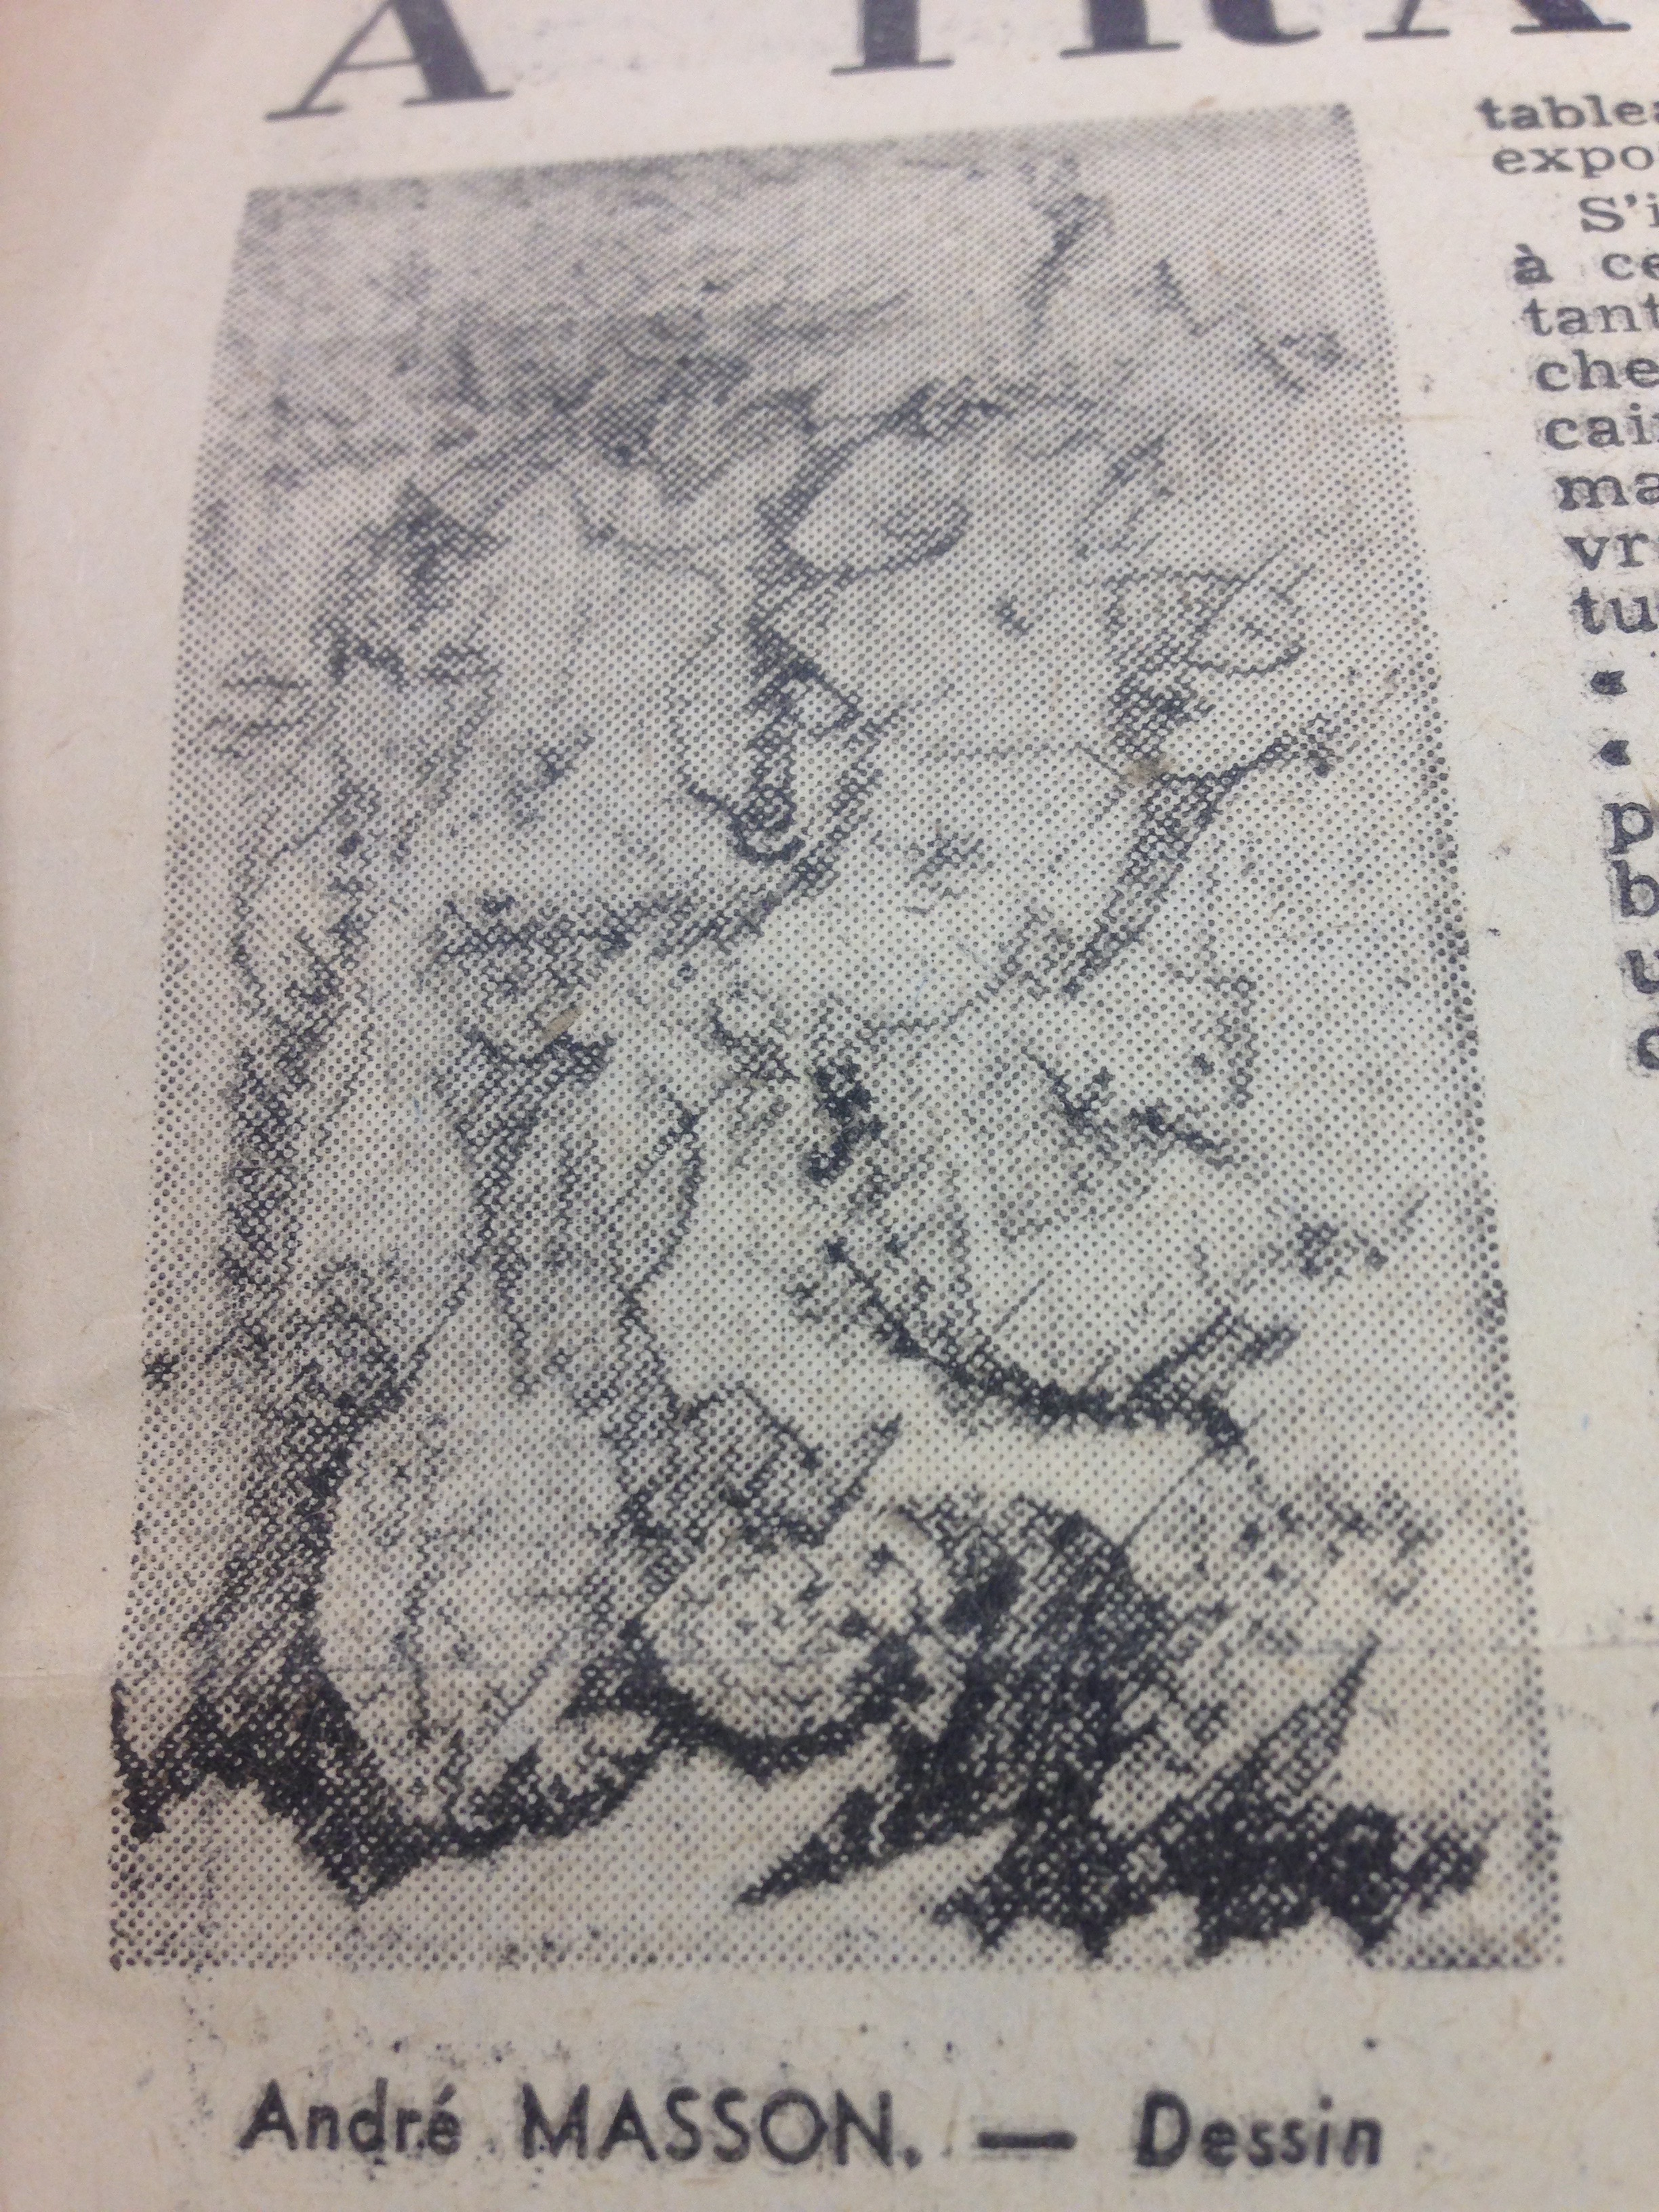
\includegraphics[width=0.75\textwidth]{dessingaleriesn669.jpg}
	\caption{\cite{realsoc}}\label{fig:Atraverslesgaleries}
\end{figure}



	Et pourtant, Masson peut-il être un représentant du réalisme socialiste ou de la politique du parti communiste, alors que sa figuration d’une réalité autre rend ambiguë la frontière entre la figuration et l’abstraction ? 
	
	\begin{quote}
	 Hors d’un trait nerveux, de rayonnements colorés, remarquables, vous ne reconnaîtrez pas Masson à son style. Ce peintre ne s’est pas laissé peindre à cette mode du graphisme en quoi l’on veut que chacun se résume. Il ne veut pas non plus être le peintre de quelques accords de couleurs. Si jamais artiste a fui le style, c’est bien lui. Aussi trouve-t-ton plus d’un tableau déconcertant dans cette exposition.\footcite{atraversgaleries}\end{quote}
	
	 Masson à contre-courant, donc. Le dessin au-dessus des lignes de la chronique n’est lui-même pas immédiatement identifiable, et c’est d’abord des figures abstraites qui apparaissent. Néanmoins, et c’est probablement en raison du choix de représenter une réalité autre, si le sujet n’est pas immédiatement identifié, il se devine. 

Il se devine par le biais de ce qui justement évoque dans un premier temps l’abstraction :les lignes, le tracé. Le corps d’une jeune femme nue en pleine nature apparaît dans les courbes des lignes. Une telle scène présenterait donc un sujet classique, mythologique ou sur la femme, deux thèmes chers à Masson, mais totalement redécouverts avec un nouveau regard de la part de l’observateur qui a deviné le sujet à la fois caché et révélé par le trait. Or, non seulement la figuration existe, mais puise son efficacité dans l’ambiguïté, mais il en de même pour le traitement des sujets : 

\begin{quote}
il s’attache à exprimer ces idées simples qui sont aussi des sensations et des spectacles d’une complexité formidable. Tant de choses tiennent-elles dans la peinture ? Il les y met, en tout cas, et trop souvent nous nous trouvions que devant un graphisme nerveux, devant quelques virgules nageant dans la couleur, devant de puissants mouvements.\footcite{atraversgaleries}\end{quote}

 
	On remarque d’ailleurs que les deux aspects sont tout autant des compliments pour Pierre Descargues : d’une part, la \enquote{simplicité}, avec des sujets au titre très bref généralement sur un sentiment, un personnage de mythologie, les femmes, les scènes de massacres. D’autre part, \enquote{des spectacles d’une complexité formidable}. Masson rechercherait-il avec une autre forme du réel une autre représentation du sublime ?  Or, si l’on regarde le dessin publié au-dessus de l’article, la simplicité apparente s’accompagne si l’on suite les traits jaillis du corps féminin une grande part de détails : la courbe de la tête de la femme penchée, les motifs autour d’elle et à ses pieds. Des personnages inachevés surgissent même dans les airs. Ils surgissent parce qu’on ne les distingue pas tout de suite, et l’on ne sait pas immédiatement s’ils sont produits par l’hallucination du spectateur ou bien réellement produits par fragments par le mouvement des traits. 

	Avec cette création de personnages, les lignes ne composent pas uniquement le sujet, mais le racontent, mais comme le ferait non pas un narrateur mais plusieurs, plus proches de la polyphonie due à des voix mélangées. Il peut ainsi paraitre paradoxal qu’à l’heure du réalisme socialiste, ce dessin, certes pleinement représentatif du geste du dessinateur en train de créer comme l’apprécie le communisme, se rapproche plutôt du dessin automatique conçu par les surréalistes. On peut se demander devant ce dessin d’André Masson si le sujet de cette jeune femme nue était réfléchi avant le geste du dessin, ou si c’est justement l’inconscient des traits qui ont formé le sujet. La référence de Descargues au traitement de la couleur est intéressante, puisque le choix du dessin justement privilégie la forme, les fameuses \enquote{quelques virgules nageant dans la couleur}. Les couleurs du dessin révèleraient-elles alors une toute autre \oe{}uvre ? Or, les couleurs sont ancrées elle-mêmes dans le tourbillon de la forme, indissociables du mouvement. Ce qui justifie le choix des \emph{Lettres françaises}, fait pour beaucoup d’artistes, mais particulièrement pour André Masson, de privilégier ses dessins et esquisses aux tableaux : le mouvement figure à la fois le tracé et la couleur. Il est la composition dans sa totalité. Pour autant, pourquoi André Masson n’incarne-t-il pas  la ligne du réalisme socialiste ? 


On se rappelle qu’en 1952, Aragon précise dans son article sur le prix Staline décerné au \emph{Premier Choc} d’André Stil non seulement la définition du réalisme socialiste, mais aussi que celui-ci peut évoquer la peinture en parlant d’un livre et réciproquement. Or, dans l’article \emph{Réalisme socialiste pas mort} de 1957, Aragon commente deux \oe{}uvres littéraires avec une distinction sur leur vocation romanesque : \enquote{Cela dit, il y a deux sortes de romans : ceux qui se racontent, comme celui de Doudintsev (2); ce dont on ne peut dire que le thème, comme celui de Polevoï}. Cette distinction est intéressante au regard des \oe{}uvres de Masson, dont le titre désignerait plutôt un thème. Pourtant, si l'on regarde la scène fantastique de la femme nue dans la nature du \emph{Dessin }publié pour la rubrique \emph{ÀTravers les galeries}quelques semaines plus tôt, peut-on être sûr que les traits ne racontent rien ? 

	Les traits vifs racontent avant même le sujet quelque chose de l’état d’André Masson en train de dessiner. Si narration il y a, elle n’est ni réfléchie ni anticipée, pour privilégier au contraire la vitesse du geste de création. D’après Bernard Noël, à propos des dessins automatiques de Masson, la vitesse c’est à la fois ce qui fait de Masson une figure emblématique du dessin automatique, tout en le mettant à part des autres artistes surréalistes : \enquote{Cette vitesse-là- celle même de l’automatisme - fait bien d’André Masson le premier peintre surréaliste, et cependant elle travaille à l’éloigner du groupe parce que l’explosante en elle-même n’est jamais fixe.} Ainsi, même avec l’empreinte indélébile du surréalisme dans ce Dessin, André Masson est à la fois une figure d’autorité sans pour autant être un modèle, puisque son style n’est pas suivi même pas les auteurs de dessins automatiques de sa génération. 

	Mais, en 1957, présenter ce \emph{Dessin} révélateur du tracé originel est sans doute la seule caractéristique commune entre André Masson et un réalisme socialiste qui n’est plus en plein essor en 1952 mais plutôt au stade de survie, comme l’induit le titre \emph{Réalisme socialiste pas mort}. Le lyrisme est cependant de première importance aussi bien dans ce \emph{Dessin} de Masson que dans ces critiques de livres réalistes socialistes par Aragon. Mais la différence notable de l’expression lyrique tient probablement au rapport avec le temps : André Masson exprime des émotions dans l’instantanéité de l’instant présent. Le sujet, cette jeune femme n’existe en tant que telle que parce que dessinée dans la vitesse du temps présent. La mobilité de son corps en témoigne, et pas un élément même parmi les personnages inachevés ou apparement naturels n’est statique. Or, la critique littéraire des \oe{}uvres soviétiques réalistes socialistes par Aragon ne crée pas le lyrisme par le mouvement vif du présent, mais par la nostalgie, le passé : 

\begin{quote}
…c’est la donnée initiale du livre, mais comment suivre le détaille leurs aventures, restituer le tragique de cette histoire, rendre le parfum de la terre russe, de ses forêts dans l’été de 1941, le paysage bouleversant et boulversé, les passages d’hommes et d’animaux sur les pistes secrètes à deux pas de l’armée d’invasion en marche ?\footcite{realsoc}\end{quote}	


Le fait que cette nostalgie soit vouée à l’URSS n’est sûrement pas anodin, et l’on pourrait presque entendre dans ce romantisme des lieux russes la propre nostalgie d’Aragon pour le pays dans son poème \emph{Hourra l’Oural} de 1934 : \enquote{C’est troublant / c’est tout à fait tremblant / Simplement sous leurs pieds la terre /s’était mise à se souvenir / L’Oural rêvait}\footcite{hourra}. Comme dans la critique du livre \emph{L’Or de Polevoï}, le lyrisme se construit autour de la terre, le symbole d’un lieu natal mais qui est aussi un espace ancré, fixe, là où les traits de Masson ne cherchent pas à retrouver le passé sacralisé. Le visage du couple, d’une femme est chez Polevoï comme dans \emph{Hourra l’Oural} mêlé aux racines russes, ce qui renforce l’imaginaire romantique autour de la terre natale, ou symboliquement natale dans le cas d’Aragon. Le trait de Masson, lui, est en partie éphémère, avec ses personnages inachevés, sans origine distincte puisque le tracé est emmêlé. Ainsi, si le lyrisme est omniprésent dans le \emph{Dessin} comme dans la critique d’\oe{}uvres réalistes socialistes, son traitement est nuancé.
%reprebdre p 102- (p16) 


	D’autre part, la critique d’Aragon repose sur la nécessité d’un héros collectif et réhabilite le genre noble par excellence, l’épique : 
	\begin{quote}
	et brusquement nous nous rendons compte que l’acte héroïque a été et ne pouvait être qu’un acte collectif, et que ce livre n’a pas été le roman de deux, trois, quatre ou cinq hommes et femmes particuliers, mais l’épopée d’un peuple, le roman d’un peuple, au sens du \emph{Roman de Thèbes}, la \emph{Chanson de Roland}.\footcite{realsoc}\end{quote}
	
	
	 Or, si l’épique est d’une part un genre peu présent dans la production littéraire contemporaine, il est aussi pour Aragon en tant que directeur des \emph{Lettres françaises} l'idée de faire du réalisme socialisme un aboutissement à la Résistance, qui fut l’origine de la création du journal. 

	André Masson n’est pas étranger à l’expression de l’acte de résistance, mais la création ne peut pas venir du collectif, mais au contraire d’un point de vue intime, puisque la liberté des traits du dessin vient de la notion de désir. C’est pourquoi la liberté est polyphonique dans les \oe{}uvres de Masson : libertaire comme dans ce \emph{Dessin}, et l’expression appuyée du corps féminin nu et la retranscription en mouvement d’un autre type de cri qui est celui de la révolte. La nature même du dessin automatique et sa remontée vers l’inconscient ne permet pas de reposer sur une dimension collective propre au réalisme socialiste. Cependant, d’un point de vue intime ou collectif, André Masson comme le réalisme socialiste cherchent à retranscrire le ressenti du peuple avant même sa représentation. 

	C’est pourquoi la finalité réclamée par Aragon dans les dernières lignes de sa critique littéraire rejoint celle du \emph{Dessin} d’André Masson et sa figuration comme ressenti du réel, et non plus son mimétisme : 
%corriger la p16 phrase de transition 
\begin{quote}
Un jour, messieurs les liquidateurs, la jeunesse de ce pays déchirera vos écrits avec ce mépris que donnent les grands enthousiasmes, ce mépris que ma génération eut pour vos prédécesseurs qui ignoraient Rimbaud au nom de Sully Prudhomme.\footcite{realsoc}\end{quote}
 
	 En réactivant la vieille querelle de Rimbaud contre les Parnassiens, Aragon sous-entend que le réalisme socialiste est méprisé, du moins en partie en France. Il l'est au profit d’autres courants littéraires privilégiés qui occupent le devant de la scène. Mais on retrouve aussi dans cette défense du réalisme socialiste les prémices de la thèse défendue en 1959 dans \emph{Savoir aime}r à propos du travail de critique : Le réalisme socialiste a pour essence l’\enquote{enthousiasme}, autrement dit ce qu’Aragon exige aussi de la critique en général.  

	Or, avec son exigence de vitesse lorsqu’il dessine, André Masson recherche lui aussi un jaillissement de l’expression au sens le plus vif. Cet élément qui est sans doute l’élément le plus fondamental du texte est aussi le plus intimement proche de l’esthétique d’André Masson : \enquote{Il ne suffit pas de dire que le feu ne brûle pas quand c’est tout un monde qui s’embrase}. Cette phrase au présent gnomique aux allures de maxime est celle mise à part des autres et qui conclut l’article. Même si la passion qu’Aragon évoque comprend avec le \enquote{monde} la dimension collective théorisée précédemment, le lieu commun des flammes rejoint les métaphores astrales de Masson permanentes dans ses écrits : si le réalisme socialiste exige une forme collective, basée sur la tradition épique mais aussi plus onirique avec la référence aux troubadours et à la performance, le lien étroit entre le concept et l’art de Masson se fait au niveau d’une réception aux attentes analogues : une certaine dévastation est attendue, un dérèglement des sens. Le lecteur d’une \oe{}uvre réaliste socialiste et un spectateur d’une \oe{}uvre de Masson doivent être à l’inverse de la passivité, ou de toute distanciation. 

	On peut d’ailleurs soupçonner Masson, lorsqu'il dessine à partir de l’intime pour produire ce mouvement conçu à partir de flux de pensées, de parler en réalité non d’un homme mais de l’homme. Or, cette passion qui répond à deux projets différents mais qui est nécessaire dans la création répond aux mêmes exigences en terme de réception, et rejoint ainsi une conception spécifique de l’homme. L’image de la flamme demeure le lieu commun du désir. Le désir est aussi l’essence même de la création de Masson. 

C’est pourquoi il ne s’agit pas en convoquant ces notions de soulèvement de passion de confondre l’art d’André Masson caractérisé par ce \emph{Dessin} avec l’idée qu' Aragon se fait du réalisme socialiste. D’abord, comme la négation à la tête du titre l’évoque, \emph{Non le réalisme socialisme n’est pas mort}, Aragon est dans une position de défense et de refus. On comprend d’ailleurs quel facteur décisif peut être l’appel aux passions pour justifier la continuité de son existence malgré cette période obscure pour le réalisme socialiste après le rapport de Khrouchtchev le 24 février 1956 où les crimes et déportations de Staline sont dénoncés pendant ce XXème Congrès de Moscou. Pourtant, les deux événéments que sont les ouvrages exaltés par Aragon rappellent aussi le synonyme que l'écrivain prête à la valeur \enquote{réaliste socialiste} :  

\begin{quote}
\enquote{la récompense du réalisme}, a depuis longtemps trouvé son fondement doctrinal dans le romantisme révolutionnaire, l'autre nom, on le sait, du réalisme socialiste.\footcite[p1012]{these}\end{quote}

Les termes de cette autre désignation induisent tout un panel d'affects qui expliquent quel déchirement interieur signfierait pour Aragon de renoncer au \enquote{réalisme socialiste}. Le réalisme socialiste est ainsi désigné sous son autre nom comme le lieu des passions par excellence et sous-entend sa visée utopique. 

% Voir Chronique du Bel Canto. (Fait)

	 Ainsi, en concluant par cette métaphore du désir, Aragon ne mentionne plus la passion autour du stalinisme, présente dans sa définition de 1952 lors de la remise du Prix Staline à André Stil. En revanche, il préserve une substance idéologique indépendante de la figure de Staline. Or, si l’on compare l’image de l’homme selon Aragon au nom de ce réalisme socialiste revisité et celui d’André Masson où du désir s’exprime une vision de l’homme, sur l’homme, on voit que de ces deux désirs aboutissent une conception idéologique proche et intime. Il n’est pas certain que les autres auteurs réalistes socialistes ou les dirigeants et militants communistes approuvent totalement la réorientation du réalisme socialiste d’Aragon, forcément plus personnelle à présent, et que ce socialisme se rapproche de la vision socialiste aussi d’André Masson sur les hommes. C’est pourquoi on peut se demander si l’origine de cette perception idéologique, créative et réceptive n’est pas due à cette conviction essentielle chez les deux hommes que l’idéologie politique naitrait de leur création, \enquote{et non pas l’inverse}\footcite{}. 
%Source web : 	http://fresques.ina.fr/jalons/fiche-media/InaEdu01226/louis-aragon.html : Aragon assit autour d’étudiants le 27 janvier 1967. (Fait)

\section{Discours récurrents des \emph{Lettres françaises} autour d’André Masson (n\degre1104- du 4 au 10 novembre 1965)}  

\subsection{Numéro des \emph{Lettres françaises} : André Masson et le Plafond de l'Odéon }


Le journal \emph{Les Lettres françaises}, qui se compose à partir d’un fil conducteur sur des thèmes spécifiques dans chaque numéro, s’arrête  sur les éléments de l’esthétique d’André Masson.  Ils font corps avec l’idée-phare du numéro.  La récurrence de topoï dans les discours des journalistes et des années pour qualifier l’art d’André Masson sert ce dessein éditorial. L’esthétique de Masson va être associée grâce aux discours des chroniqueurs, à l’idéologie politique du journal. Le rapport d’André Masson aux \emph{Lettres Françaises} est aussi profond que multiple : d’abord comme grand lecteur lors de son exil aux Etats-Unis, puis comme le chroniqueur qu'il deviendra dans certains numéros : 

\begin{quote}
Votre lettre m’a fait le plus grand plaisir. Je vous prie de m’excuser : j’ai tant tardé à vous écrire que je recevais les “lettres Françaises“ (la seule revue à cette heure qui nous rappelle que quelque fois les Français savent penser et écrire) », « « J’ai lu votre très beau texte : “La Pampa“ dans le dernier numéro que j’ai reçu des L.F- Si cette revue ne paraît plus ce sera désolant.\footcite[p478]{anneessurrealistes}\end{quote}
 
	Ainsi, \emph{Les Lettres françaises }figurent pour l’artiste le dernier moyen d’avoir encore foi en l’humanisme. Cette réception n’est donc pas anodine, surtout à la lumière des articles de grands chroniqueurs du journal lorsque ces derniers, même une vingtaine d’année plus tard, parleront de Masson. De même, cette réception très forte chez Masson et qui voit en ce journal le dernier rempart de la pensée peut-être une expérience déterminante lorsque lui-même écrit un article pour \emph{Les Lettres françaises}, ce qui arrive dès les années 50. Plus précisément, les articles de Masson, dont la qualité littéraire est reconnue par le journal lui-même en plus de son immense culture, ont pour vocation généralement par la revendication d’une certaine vision de l’art. Ce travail dans les analyses de Masson passe généralement à travers la figure d’artistes comme Turner, Cézanne. La figure de Cézanne en particulier dépasse l’hommage, le journal même une dizaine d’années plus tard, composera tout un engagement pour sauvegarder la mémoire de l’artiste, oubliée dans sa région d’origine. 

	%Intertitre ? 

On touche déjà à des questions qui relèvent de choix d’engagements politiques du journal. Sans compter les grandes enquêtes dont la problématique est centrée sur l’art dans plusieurs numéros. Masson y apparaît comme l’un des discrets mais toujours fidèles intervenants. Il va s’agir de constater à quel point l’esthétique d’André Masson se cofonf dans ce fil conducteur qu'est l’idéologie de la politique éditoriale des \emph{Lettres françaises}. C’est pourquoi nous pouvons d’abord nous pencher sur ces topoï récurrents, pour ne pas dire persistants, qu’auront les journalistes des \emph{Lettres françaises} vis-à-vis d’André Masson. D’autant plus que la plupart de ces journalistes précisent bien le connaître personnellement, ce qui inclut l’aspect individuel, humain de l’artiste dans leur analyse de son art.

	A ce titre, le numéro sur le plafond de Masson pour le théâtre de l’Odéon est particulièrement révélateur. Il comprend non seulement l’article de Georges Boudaille, mais aussi les notes d’André Masson sur ce même sujet. D’autant plus que les deux articles co-existent sur la même page, à la suite des esquisses du plafond. Leur titre, \emph{Les premières esquisses d’André Masson} correspond naturellement avec l’article \emph{Notes de travail d’André Masson} et leur état commun de dimension inachevée. 

	\begin{figure}[H]
   \centering
   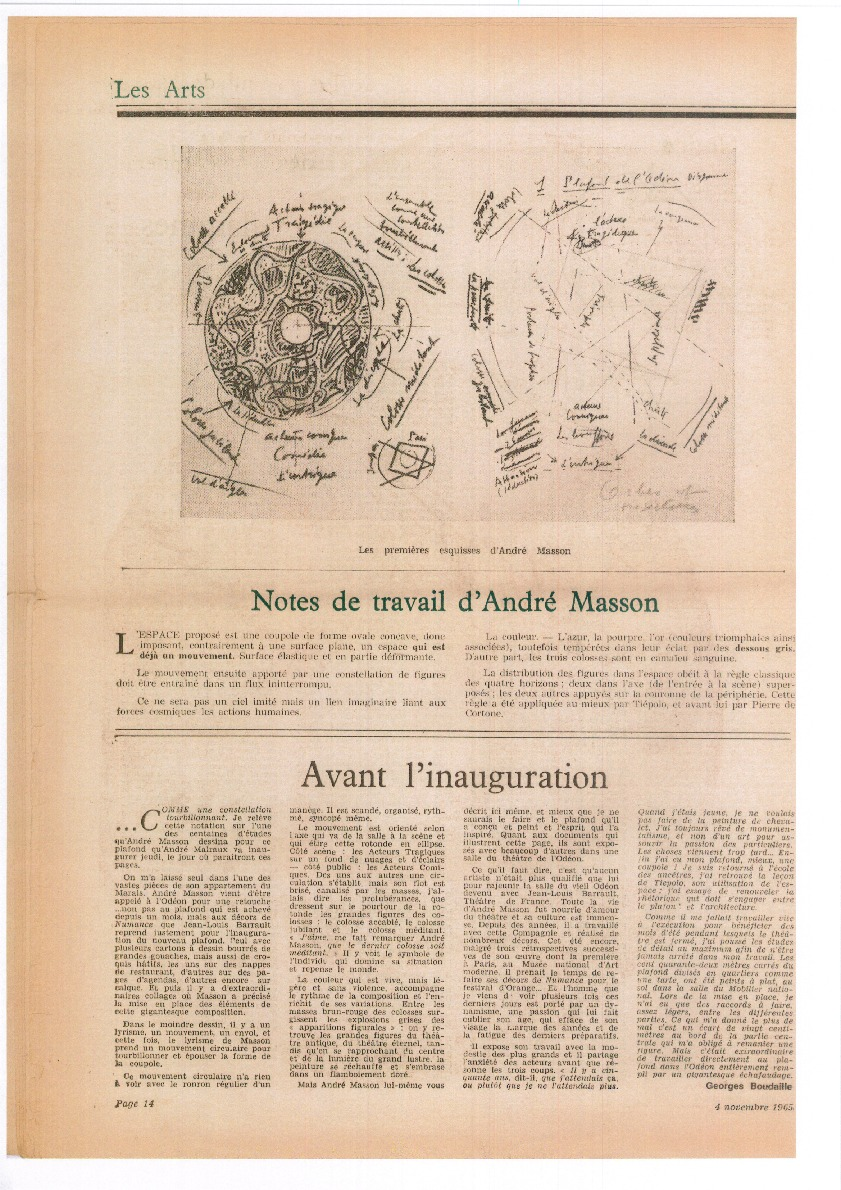
\includegraphics[width=0.75\textwidth]{massonesquissesplafond.jpg}
	\caption{\cite{plafondodeon}}\label{fig:Notesdetravail}
\end{figure}



Même l’article de Georges Boudaille,\emph{Avant l’inauguration}\footcite{avantinauguration}, joue sur une forme de genèse. \emph{Ces notes de travail d’André Masson}, citées au centre de la page comme le point fixe d’une image, accrochent particulièrement le regard avec le choix éditorial de colorer le titre en vert, de même que la banderole autour du titre des \emph{Lettres françaises}. Reste à savoir si les fragments mis en gras plutôt que d’autres respectent une différence de marque typographique des notes originelles de Masson, ou si le numéro a voulu accentuer la réflexion de Masson sur son travail en extrayant des notions-phares dans le texte. L’importance de cette distinction typographique n’est pas négligeable, en raison du choix de colorer le titre de cet article et de termes spéicifiques. Avec ce dispositif, on prend en considération l’enjeu majeur qu’ Aragon lui attriue en tant que directeur de journal: 

\begin{quote}
L’abondance de ces variations graphiques, sur lesquelles Aragon a veillé, témoigne de son intérêt de grand directeur de journal pour la dimension matérielle du livre et les effets signifiants qui en découlent. On sait le lien d’Aragon avec les typographes des \emph{Lettres françaises }et de nombreuses photos le montrent travaillant avec eux au marbre du journal.\footcite[p333]{vasseviere}	
\end{quote}

Ainsi ces deux fragments précisément mis en gras : \enquote{qui est déjà un mouvement} à propos de l’espace oval du plafond, et  les \enquote{dessous gris} pour tempérer la vivacité des couleurs rouge et or, rejoignent la valeur signifiante évoquée par Maryse Vassevière. En outre, le premier fragment est révélateur non seulement d’une caractéristique essentielle dans l’esthétique d’André Masson, peut-être même sa principale, mais aussi d’un topos récurrent chez les critiques pour qualifier Masson : \enquote{qui est déjà un mouvement}. L’adverbe \enquote{déjà} sous-entend que la forme ovale anticipe le désir créateur de Masson de créer le mouvement dans l’espace. Et, comme par un jeu de dialogue interne ininterrompu, signifié par les points de suspension à l’ouverture de l’article, facilité par la proximité de ces articles voisins, Georges Boudaille entame son propre article avec d’autres termes de Masson. Ils reprennent cette exigence fondamentale que doit être le mouvement du participe présent:\enquote{\emph{Comme une constellation tourbillonnant}}.On remarque la portée dévastatrice que suggère la métaphore du tourbillon. 


% mettre l'illustration du théâtre de lOdéon. 


	En outre, il  ressort de cette combinaison de la \enquote{constellation} et du tourbillon la volonté de faire prévaloir dans son langage la fonction poétique : une écriture, pourtant à l’état de \enquote{notes}, et que l’on attendrait par conséquent plutôt résiduelle, schématique. C’est d’ailleurs bel et bien le mouvement qui fascine Georges Boudaille chez André Masson, comme l’illustre la gradation ascendante des quelques lignes de ce paragraphe : \enquote{Dans le moindre dessin, il y a un lyrisme, un mouvement, un envol, et cette fois, le lyrisme de Masson prend un mouvement circulaire pour tourbillonner et épouser la forme de la coupole}. 

	Ainsi, la forme ovale, en rencontrant les formes elles-mêmes agitées de Masson ne crée pas seulement ce mouvement qui existe \enquote{déjà}, mais provoque en revanche ce tourbillon induit dans la citation que Boudaille extrait des notes de Masson et qui reparait dans sa propre écriture. Cette image du tourbillon induit une idée de force de cet élément naturel dans le paragraphe suivant, axé lui aussi sur le mouvement : \enquote{Ce mouvement circulaire n’a rien à voir avec le ronron régulier d’un manège. Il est scandé, organisé, rythmé, syncopé même}. En somme, le contraire de la monotonie, et l’agitation réfléchie, puisque André Masson en organisant le mouvement travaille surtout à l’orientation, également circulaire, du regard : \enquote{“\emph{J’aime, me fait remarquer André Masson, que le dernier colosse soit méditant“}. Il y voit le symbole de l’individu qui domine sa situation et repense le monde.} Ainsi, la notion fondamentale du mouvement dans une esthétique aussi difficilement identifiable d’une \oe{}uvre à l’autre chez Masson, comme ne le manqueront pas de le souligner dans d’autres numéros les critiques, comprend lui-mêmes deux valeurs essentielles dans sa création : Le lyrisme syncopé à l’agitation, et sa finalité tournée vers l’homme. 

	En somme, un portrait d’une idée de l’homme figuré par le mouvement, comme le sous-entend au plafond de l’Odéon la fin du cercle sur la figure du penseur. Le mouvement d’André Masson ne se limite donc pas à la question esthétique, puisque toute l’organisation de celui-ci suit un fil humaniste, dans cet exemple du plafond de l’Odéon : \enquote{Ce ne sera pas un ciel imité mais un lien imaginaire liant aux forces cosmiques les actions humaines}, mettent en garde ses \emph{Notes de travail} dans l’article précédent. Cette orientation se rapproche d’un idéal, lorsqu’on se rappelle de la désolation d’André Masson pendant la 2nd Guerre Mondiale, où, depuis les Etats-Unis, la seule trace de pensée en Europe résidait dans la revue \emph{Les Lettres françaises}. Masson établit donc un portrait de l’homme par le mouvement puisqu’il ne peut concevoir celui-ci qu’à travers sa faculté de penser. 

En outre, Georges Boudaille respecte la structure de l'article  \emph{Notes de travail d’André Masson} qui précèdent son article, puisque qu’après l’analyse du mouvement chez Masson, Boudaille évoque la couleur : \enquote{La couleur qui est vive, mais légère et sans violence, accompagne le rythme de la composition et l’enrichit de ses variations}. 

%mettre cet article en annexe

	On reconnaît dans cette description la tempérance du rouge et de l’or permise par les \emph{dessous gris}, l’autre fragment en gras dans le texte. D’autre part, cette description sur la combinaison de couleurs vives sur un fond tempéré évoque tant chez Masson que chez Boudaille le principe de la devise : \enquote{La couleur . — L’azur, le pourpre, l’or (couleurs triomphales ainsi associées), toutefois tempérées dans leur éclat par des \textbf{dessous gris.}}L’agitation des couleurs maitrisées par la tempérance, une forme de raisonnement. La réflexion des couleurs, tout aussi minutieusement détaillée bien que n’étant pas visible dans les esquisses du numéro, est finalement fondée exactement sur le même raisonnement que pour la forme du mouvement : L’éclatement doit apparaitre avec la même énergie que le mouvement des personnages, éclater au regard, mais le lyrisme n’est possible qu’avec l’harmonie de ses couleurs vives avec le fond gris.


	C’est pourquoi il ne s’agit pas tant en soit de limiter l’agitation de la ronde que l’orienter vers un idéal de la Pensée, c’est-à-dire la faculté de l’homme à perpétuellement penser, avec ses forces et ses contradictions, mais dans une finalité humaniste, donc maitrisée. On pourrait presque remplacer \enquote{peinture} par \enquote{pensée} lorsque Boudaille conclut ainsi son paragraphe sur la couleur : \enquote{tandis qu’en se rapprochant du centre et de la lumière du grand lustre, la peinture se réchauffe et s’embrase dans un flamboiement doré.}  On trouve ici une idée d’apothéose, qui n’est pas sans rappeler l’esthétique sublime du XVIIIèmme avec la dimension spectaculaire qu’elle comporte. L’apothéose de la pensée passe également par l’organisation lorsque Masson choisit d’arrêter le regard avec pour dernier personnage l’homme qui médite : Il signifie le mouvement de la pensée par excellence. 


En outre, Georges Boudaille use de cette force du mouvement comme tourbillonnons seulement pour analyser les dessins et le plafond de l’Odéon d’André Masson, mais également pour décrire comment cette force rejaillit sur l’artiste : \enquote{aucun artiste n’était plus qualifié que lui pour rajeunir le théâtre du vieil Odéon}, \enquote{Et l’homme que je viens de voir plusieurs fois ces derniers jours est porté par un dynamisme, une passion qui lui fait oublier son âge, qui efface de son visage la marque des années et la fatigue des derniers préparatifs.}. Ainsi, par jeux de reflets, l’art basé sur le mouvement influence l’individu, et non l’inverse. 

	C’est grâce au dynamise recherché dans son \oe{}uvre qu’André Masson en tant qu’individu devient lui-même un être en mouvement, jeune, c’est-à-dire ici perpétuellement vivant. C’est d’ailleurs avant de rapporter le discours de Masson pour conclure sa critique, de même qu’il l’avait débutée avec des mots de l’artiste, Boudaille le compare à une autre branche artistique, un comédien : \enquote{Il expose son travail avec la modestie des plus grands et il partage l’anxiété des acteurs avant que résonne les trois coups} : Cette théâtralité dans l’écriture de Boudaille lie cette valeur de la jeunesse attribuée à André Masson à une certaine forme d’innocence, une tempérance qui ne peut qu’évoquer les \enquote{dessous gris}, cette sagesse, qu’il recommandait à ses couleurs vives. Dans ses paroles rapportées, André Mason mêle d’ailleurs la rigueur exigée pour travailler sur le plafond, « j’ai poussé les études de détail au maximum afin de n’être jamais arrêté dans mon travail » à une forme d’extase procurée par son art, \enquote{Mais c’était extraordinaire de travailler directement au plafond dans l’Odéon entièrement rempli par un gigantesque échafaudage.}

	Ainsi, à l’image d’une devise, cette agitation raisonnée provoque un écho entre les \emph{Notes de travail d’André Masson} et la critique de Boudaille, elle-même largement partagée entre l’analyse de Boudaille et les paroles rapportées de Masson. Mais ce \enquote{mouvement perpétuel} qui figure l’homme en tant que penseur ne peut que sous-entendre une idéologie politique dans sa démarche esthétique et se rapprocher des problématiques d’Aragon. En particulier autour du devenir du réalisme socialiste. Les marques typographiques sont discrètes, mais tout de mêmes immédiatement visibles avant la lecture. Ses marques éditoriales, en distinguant un choix de mots très précis, ne peuvent que le rappeler. 

	Cette caractéristique principale du mouvement, qui est peut-être paradoxalement l’élément qui rend les \oe{}uvres de Masson atypiques  (comment reconnaitre immédiatement une \oe{}uvre d’André Masson que l’on a jamais vu ?), les journalistes des Lettres françaises ne se contentent pas de la souligner. 

	\subsection{Article \emph{André Masson à Lyon} par Gérard Guillot }

 Nous avons vu les valeurs idéologiques du numéro de novembre 1965 que suggéraient d’après ses esquisses sur le plafond de l’Odéon. On peut à présent étudier quel autre axe idéologique cette esthétique du mouvement est analysée en Juillet 1967, à l’occasion d’une exposition d’André Masson à Lyon. Dans son article \emph{André Masson à Lyon}\footcite{massonlyon}, Gérard Guillot fait de ce mouvement un signe de liberté : \enquote{il faut aller à la rencontre d’André Masson au musée de Lyon; il faut aller dialoguer avec ses toiles et respirer leur grand souffle de liberté, celle de l’esprit, du c\oe{}ur, des mouvements et des sens !}. 

\begin{figure}[H]
   \centering
   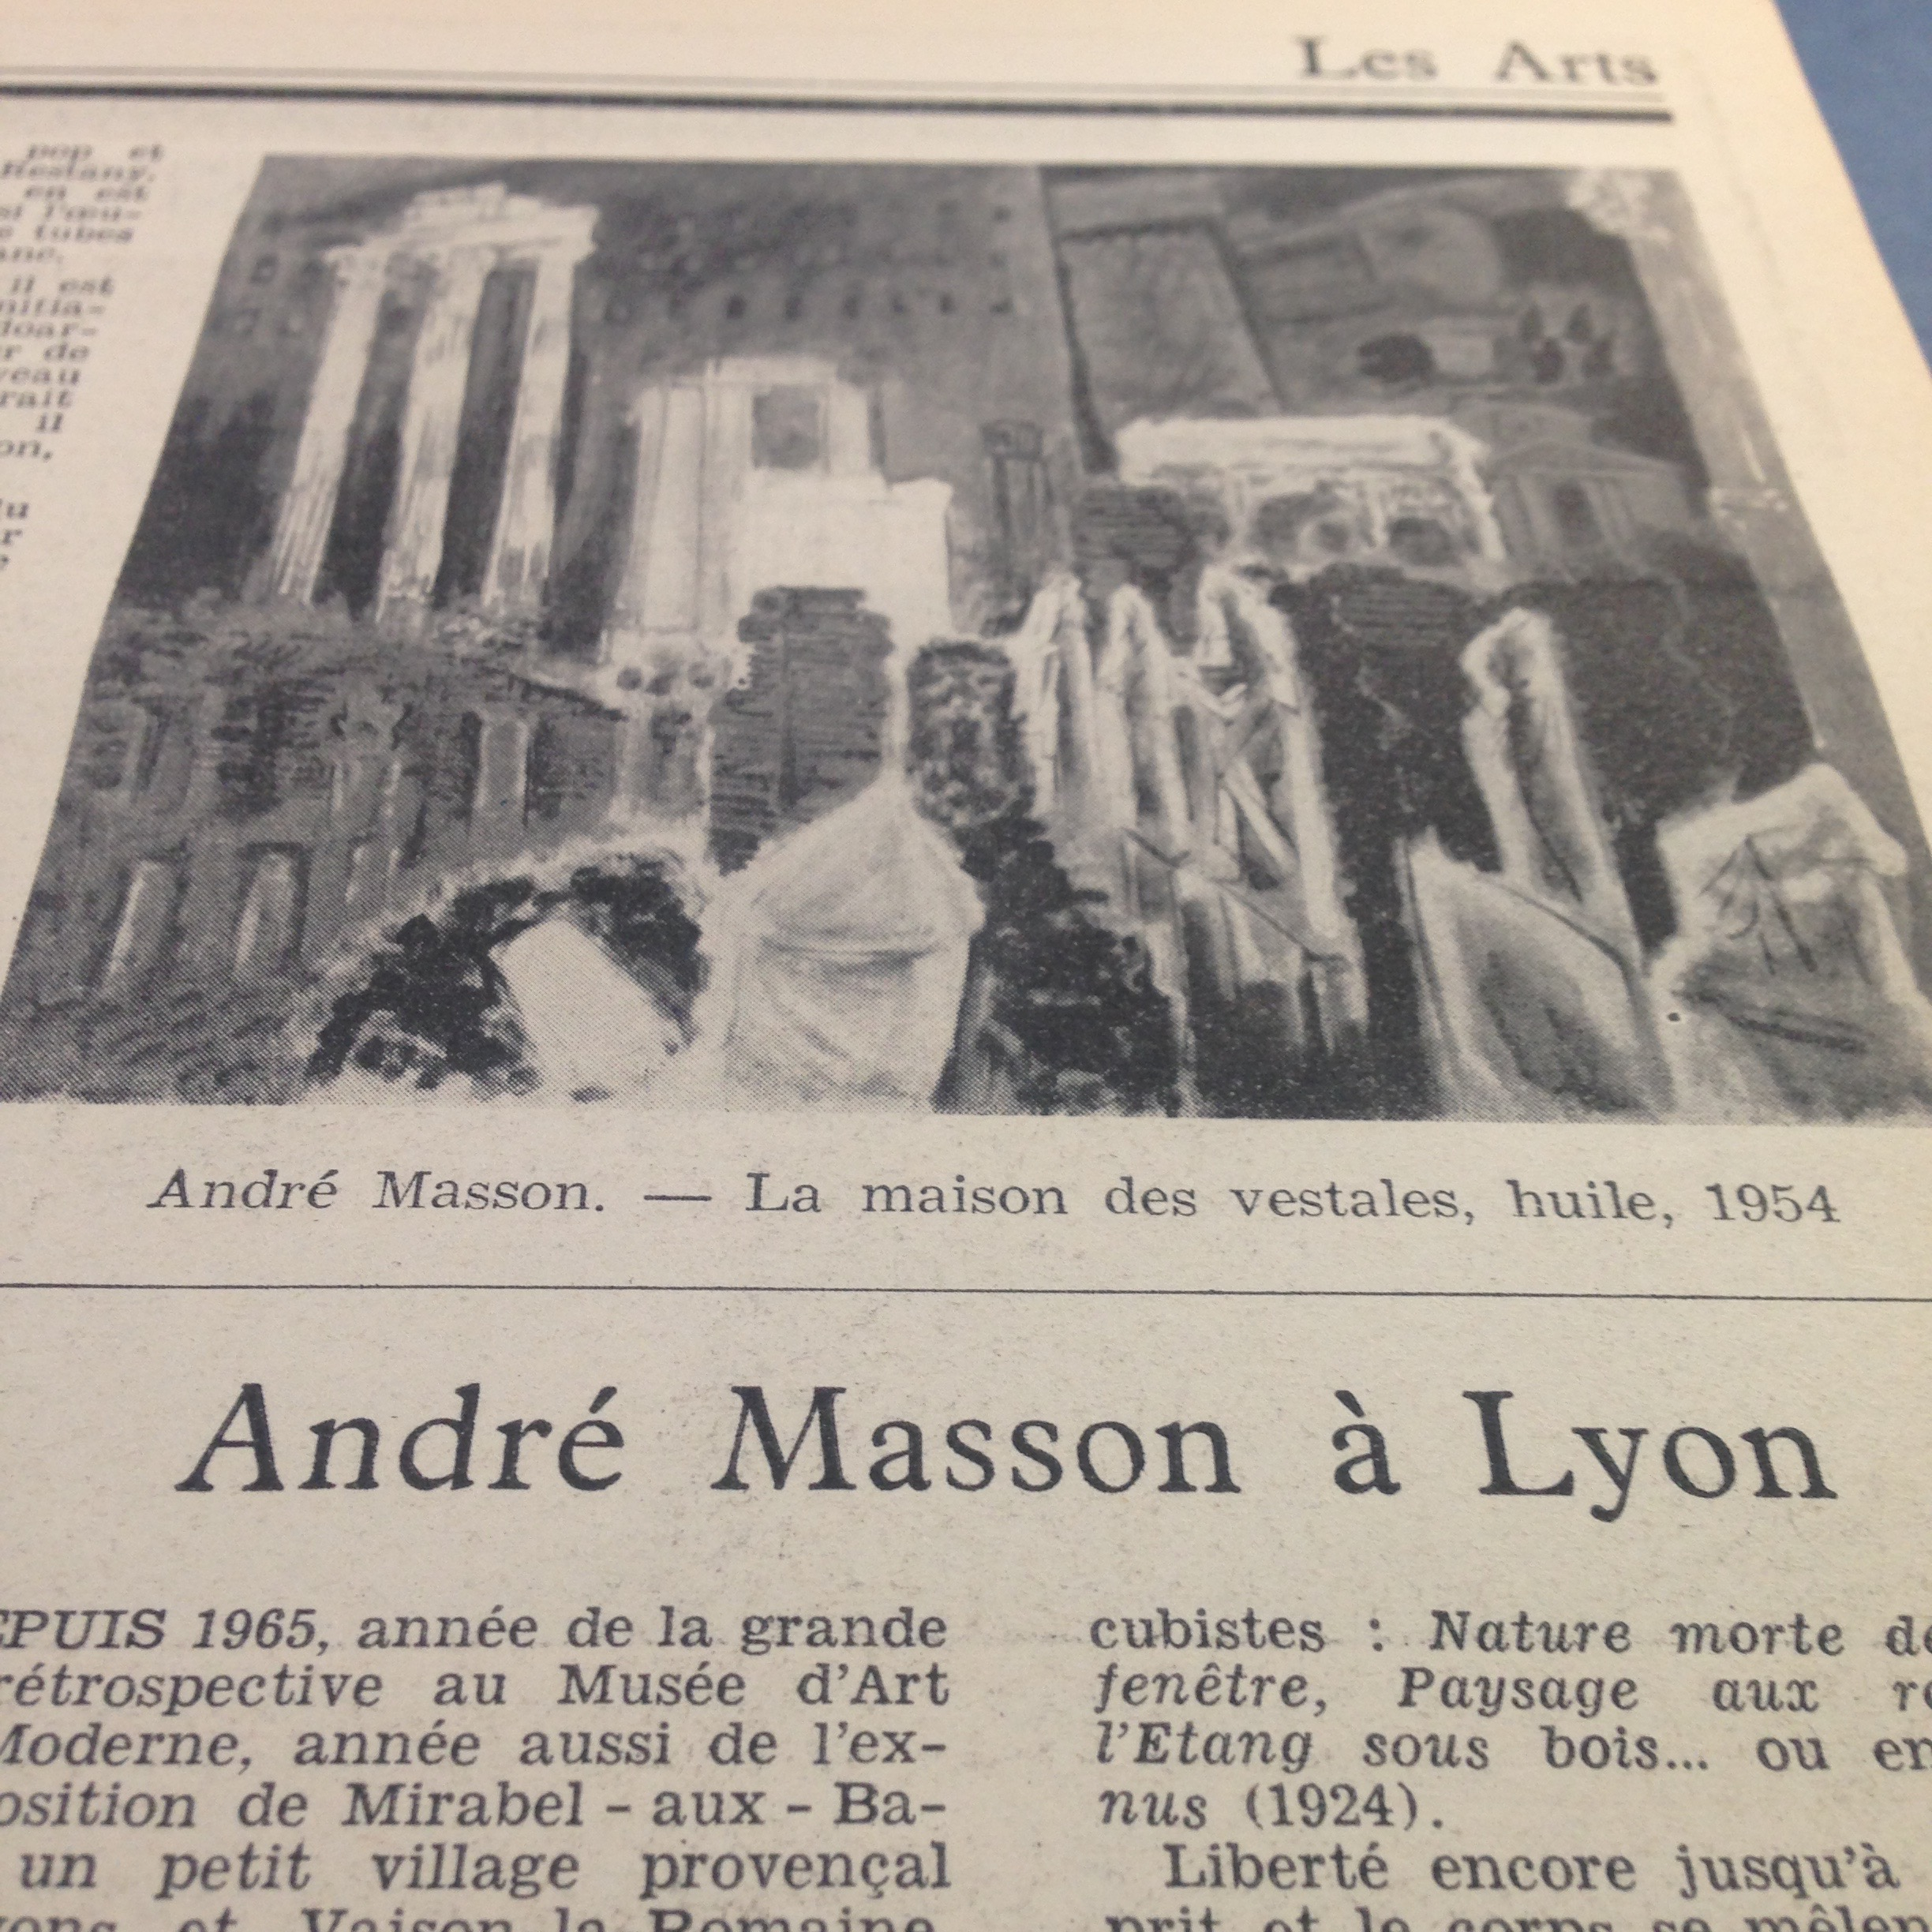
\includegraphics[width=0.75\textwidth]{imagen1190.jpg}
	\caption{\cite{massonlyon}}\label{fig:MassonLyon}
\end{figure}

	Non seulement le sème du mouvement persiste, mais il est l’un des éléments qui insuffle cet état de \enquote{liberté}. De même que \enquote{l’esprit}, dont nous avons vu dans l’organisation du plafond de l’Odéon quelle haute estime et même exigence en a Masson vis-à-vis de son art et de l’homme en général, la faculté de penser est une fois encore juxtaposée au mouvement. C’est presque une expérience synésthésique avec l’\oe{}uvre de Masson, puisque sa faculté de parler à tous les sens ouvre un \enquote{dialogue} avec le spectateur. Cette figure de Masson comme un être libre n’équivaut pas seulement à cette totale expression des sens, mais se lie à une certaine indépendance d’André Masson, atypique en tant qu’artiste malgré son appartenance à des mouvements majeurs. Cette dimension insaisissable resort lorsque Guillot associe André Masson et Jacques Prévert : 
\begin{quote}
Mais, même au c\oe{}ur au surréalisme, André Masson est resté un être “libre“; un peintre “en liberté“. Et je n’ai pu m’empêcher de comparer la position d’André Masson face à la peinture surréaliste à celle de Jacques Prévert face à la littérature ou la poésie surréaliste. Tous deux fidèles à la liberté totale et à l’absence de toutes entraves prônées par le surréalisme, ne “ sortent“ en définitive du surréalisme que parce que, précisément, ils ont su s’en sortir; ils n’en sont issus que parce qu’inconditionnels face à la grande doctrine du mouvement, ils surent s’en échapper!\footcite{massonlyon}\end{quote}
  
Ce rapprochement avec Prévert pour signifier la liberté est d’autant plus symbolique que Prévert en apparait comme l’un des plus grands défenseurs, et grand pratiquant du collage, poétique et artistique plus généralement : \enquote{L’oiseau seul et affolé / L’oiseau qui voudrait vivre/ L’oiseau qui voudrait chanter / L’oiseau qui voudrait crier}. Ces vers sont imbriqués dans un assemblage de collages, dépourvu d’oiseau mais avec d’autres signes pour renouer au symbole de la liberté. En particulier le cheval ailé perché sur l’un des monuments d’une photographie de ville d’où émane une lumière comme fond du collage. Une fleur suspendue en l’air, une seconde posée sur l’une des têtes dédoublées du poète en photo et une fée dans les airs en face du cheval. Avec ce dédoublement de signes et de photos du poète, c’est l’assemblage qui le désigne en tant que l’oiseau des vers. Celui qui aspire à la liberté, contre les signes d’oppressions tels que le panneau \enquote{arrêt}. 

	
	 Guillot confirme d’ailleurs ce rapport au corps dans la création chez Masson : \enquote{Liberté encore jusqu’à ce que l’esprit et le corps se mêlent, jusqu’à la réalité et l’imaginaire s’allient}\footcite{massonlyon}. 

	Ainsi, le mouvement des lignes chez Masson est tel que se mêlent l’organique et l’onirique jusqu’à rendre l’un et l’autre indistincts. Cette faculté d’échapper à la catégorisation va jusqu’à rendre selon Guillot les \oe{}uvres de Masson libres totalement, c’est-à-dire ressenties comme telles au seul regard du spectateur : 

	\begin{quote}
	Enfin, il y a ces toiles libres d’elles-mêmes et libres de toute influencer indépendantes et grandes ouvertes sur nos regards. Inclassables comme des expériences  uniques mais indispensables à contempler pour tous ceux qui veulent connaitre tous les méandres, tous les détours, tous les repentirs de cette \oe{}uvre puissante, attentive et courageuse… 	
	\end{quote}
 
	 La personnalisation des \oe{}uvres dans la critique de Guillot induit déjà un dépassement de l’esthétique en tant que tel, en sous-entendant que celle-ci est travaillée en fonction d’une certaine observation des hommes. Et peut-être aussi avec l’attribut « courageuse » d’une image de ce que peut être l’homme, immédiatement perceptible par le spectateur.  

En outre, les oeuvres de Masson citées par Guillot pour illustrer cette théorie sont particulièrement représentatives de cette capacité que possède Masson à échapper à la catégorisation : \emph{Tristesse d’une journée de printemps}, conçue en 1956 et composée de sable, tend vers l’abstraction et pourtant son titre préfigure immédiatement le sentiment, structuré selon l’imaginaire du peintre. 

%Mettre illustration "Tristesse d'une journée de printemps": source : André MASSON « TRISTESSE D’UNE JOURNEE DE PRINTEMPS », 1955 - Sable et pigments sur toile, signée en haut à droite, datée et titrée deux fois au dos et sur le châssis - 100 x 81 cm - Provenance : - Galerie Louise Leiris, Paris - Galerie de Seine, Paris - Collection Serge Varène, Paris.

\begin{figure}[H]
   \centering
   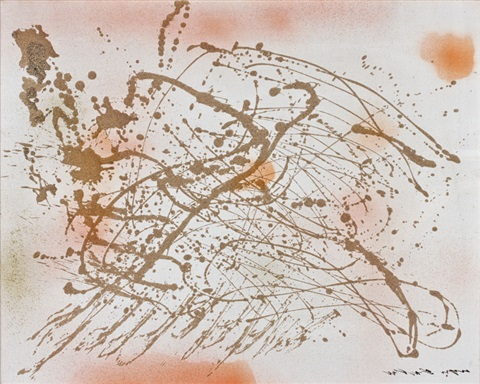
\includegraphics[width=0.75\textwidth]{tristessedunejourneedeprintemps.jpg}
	\caption{\cite{tristesse}}\label{fig:Tristessedunejourneedeprintemps}
\end{figure}

D’autre part, Masson exprime plusieurs fois dans ses \emph{Correspondances} sa réticence pour l’abstrait, qu’il juge trop limité : 

\begin{quote}
Pour moi l’observation de la nature demeure essentielle. Delacroix disait : que la nature était son “ dictionnaire“. Je n’ai jamais pensé autrement. On ne peut rien inventer de toutes pièces et les \oe{}uvres les plus imaginées sont durables dans la mesure où elles restent d’accord avec l’Univers. C’est pour cela que je ne puis accepter, personnellement d’être appelé “abstrait“. Une \oe{}uvre abstraite en peinture serait une \oe{}uvre dans laquelle il n’y aurait aucune allusion à ce qu’on nomme les 4 éléments et les 3 Règnes. Une \oe{}uvre qui ne rappellerait ni les végétaux, ni les animaux, ni l’eau ni le feu, ni la terre ni les cieux ! Mais alors le meilleur tableau abstrait c’est un manuel de géométrie !\footcite[p464]{anneessurrealistes}\end{quote}
 
	La \enquote{liberté }de l’art de Masson particulièrement manifeste pour le chroniqueur Guillot dans cette exposition à Lyon tiendrait donc en partie à échapper à la catégorisation, et ce par le mouvement. \emph{Tristesse d’une journée de printemps} figure le sentiment par le mouvement du sable qui crée la forme, avec des traits tantôt fins tantôt épais à partir des lignes. D’autre part, l'usage du sable ne peut qu’évoquer cette pratique du collage louée par Aragon dès 1939 dans son texte \emph{La peinture au défi}:
\begin{quote}
Tous les peintres qu’on a pu appeler surréalistes, cela aussi est significatif, ont employé le collage au moins passagèrement. […] André Masson a utilisé le sable et la plume, donnant avec celle-ci un effet qui rappelle les anciennes étoffes péruviennes.\footcite[p78]{ecritssurla}\end{quote}	

 	 Aragon et André Masson ont tous les deux en commun une certaine réticence vis-à-vis de la toile et la peinture. Tout du moins, il s’agit pour l’écrivain et le peintre de ne pas nécessairement privilégier cette technique. 

	Chez Aragon, cette conception rappelle irrémédiablement son passé dadaïste, puisque le mouvement dada tient dans ses Manifestes de 1916 et 1918, ainsi que dans les revues, à abolir la toile, et avec elle l’autorité de l’art. Conception forcément politique, puisqu’elle implique un renversement, une réorganisation des valeurs sociales établies. Mais on peut supposer que cette réévaluation de l’usage de la peinture à l’huile perdure même une quarantaine d’année plus tard, comme un héritage resté du l’expérience, quand Aragon déclare en 1960 : 

\begin{quote}
Il ne me semble pas que la gravité de la démarche picturale tienne à l’emploi de l’huile uniquement. Et personnellement, on le sait, j’ai peu de goût pour l’usage abstrait de ce liquide : on ne s’étonnera pas que j’apporte au moins le même sérieux à examiner la démarche du colleur de journaux découpés faisant des paysages lisibles, que d’autres mettent à discuter du non-dire à l’huile.\footcite{hoffmeister}\end{quote}
 

	 On peut s’arrêter sur la qualification de la peinture à l’huile comme \enquote{abstraite}. Contrairement aux choix du collage, et celui des objets eux-mêmes. Ainsi, même quand le réalisme socialiste n’est plut tout à fait à l’ordre du jour dans l’art d’Aragon, il reste cette dimension réaliste dans ses propres \oe{}uvres comme exigence première, et cette « gravité » de l’art nécessaire pour l’exprimer.

En outre, on peut établir une analogie entre l’écriture de l’article de Guillot lorsqu'il évolue les effets de cette \enquote{liberté}dans les \oe{}uvres de l’exposition. Sans oublier les métaphores du tourbillon dans l’article de Boudaille sur le plafond de l’Odéon en novembre 65: 

 \begin{quote}
Ce seront ensuite aux formes que Masson rendra la liberté : elles éclatent, s’engendrent les unes les autres, se déchainent, font voler en minces particules un univers pourtant déjà très tourmenté…Ainsi cette merveilleuse \emph{Constellation érotique} (1961), dans laquelle Masson déploie tout son lyrisme, tout son délire musical et coloré.(\emph{Couple dans la nuit}, 1958, \emph{Constellation des amants}, 1958)	
\end{quote}

	Tant par les titres des \oe{}uvres mentionnées que par le retour chez un autre chroniqueur du mouvement comme tourbillon, Guillot rejoint l’image de Boudaille ouverte dans son article de 65 avec les propres mots de Masson : \enquote{Comme une constellation tourbillonnant}\footcite{avantinauguration}. De cette image omniprésente ressort à la fois une forme de lyrisme cohérente avec le titre des oeuvres autour de la \enquote{constellation}dans le rapport des amants entre eux, romantique ou érotique. 

Ce lyrisme revendiqué s’accompagne aussi de cette force subversive qu’est le tourbillon. D’autant plus que les titres de Masson désignent clairement leur thème autour de l’homme, avec une figuration de lignes mouvantes qui laisse deviner sa présence. Sa masse corporelle est détournée au profit de ses lignes de force. Cependant, Guillot n’omet pas de rappeler que cette conception de la liberté esthétique, et libertaire dans ses nombreuses \oe{}uvres autour de l’érotisme, touche aussi aux faits politiques : 

\begin{quote}
Mais ce baroquisme tumultueux et orgiaque, cette écriture flamboyante et charnelle n’éloignent pas André Masson de notre monde, du monde. En homme libre, il s’inquiète de l’absence de liberté des autres…en Espagne, pendant la dernière guerre. Grande composition sur la \emph{Résistance} (1944) ou admirable ensemble de la \emph{Curée} (1944), Guerre des paysans, vaste évocation de la guerre des paysans allemands pendant la Renaissance (peinte en 1961) ou \emph{Délire lansquenet au calvaire} (1964) se partagent les préoccupations politiques du peintre…\footcite{massonlyon}\end{quote}
 
	Cette référence au baroque, le courant artistique par référence lié au mouvement confirme l’esthétique particulière de Masson en l’associant à l’attribut \enquote{tumultueux}, et cette fois à dessein d’enjeux politiques. On y retrouve l'allusion à la guerre civile d’Espagne, que Masson a vécu, lorsqu’il quitte Tossa del Mar pour Barcelone en Juillet 1936. Ou encore sa toile en hommage l’éloge à la Résistance pendant son exil contraint par sécurité envers sa famille juin aux Etats-Unis. Une forte attirance pour le thème des révolutions se dessine ainsi au cours de ses propres migrations. 

La représentation directe des hommes et des peuples est ainsi détournée  au profit de leur expression de révolte. Dans \emph{Guerre de paysans}, un arrière-plan rouge vif aux teintes agitées accueille des personnages squelettiques dont la principale caractéristique tant du grand personnage à chapeau, fantomatique, au corps constitué d’une ligne et à la tête carrée que de son voisin grisâtre miniature aux bras écartés dans le bas-droit de la toile, c’est leur bouche grande ouverte. Cette fonction radicalement expressive traversée de lignes blanches et de multiples formes plutôt fantastiques fait surgir un cri de révolte dont la dimension intemporelle des personnages fantastiques dépasse l’époque de la Renaissance. La toile ne dénonce pas tant le cri de révolte manifeste, c’est bien un idéal de cette représentation du peuple auquel aspire le \enquote{baroquisme tumultueux} d’André Masson.

\begin{figure}[H]
   \centering
   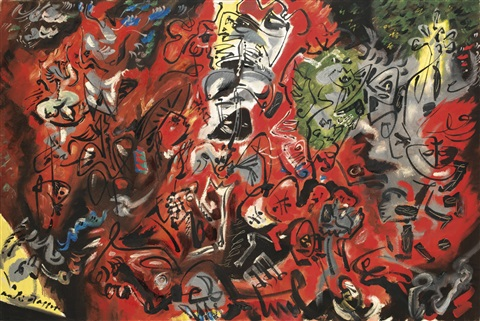
\includegraphics[width=0.75\textwidth]{laguerredespysans.jpg}
	\caption{\cite{massonlyon}}\label{fig:Guerre des paysans}
\end{figure}

%Source image : LA GUERRE DES PAYSANS , 1963- Support : oil-Taille :87,1 x 135,7 cm. (34.3 x 53.4 in)-

	 Ainsi, c’est par une ultime allusion à l’une des grandes \oe{}uvres de Masson que Gérard Guillot conclut sur cette révélation que doit être cette exposition du peintre à Lyon : \enquote{Sur une des routes vers le Sud, l’exposition André Masson doit être une étape solaire : des miroirs en liberté font exploser les limites de notre labyrinthe !} L’image \enquote{des miroirs en liberté}confirme cette vocation presque paradoxale chez Masson de représenter l’homme, plus précisément l’identité en perpétuelle mouvance de l’homme, par une dimension fantastique.

	En outre, la conclusion sur le corps squelettique \emph{Le labyrinthe} de 1938 illustre le regard très réfléchi de Masson sur l’homme dans son art, à l’image de son achèvement du plafond de l’Odéon par la figure du penseur comme le souligne Bernard Noël : \enquote{La mythologie qu’élabore André Masson compose une sorte d’encyclopédie plastique de sa pensée}\footcite[p73]{noel}. Et, comme le signifiait symboliquement le regard sur l’homme en train de penser sur le plafond de l’Odéon, avec l’\oe{}uvre du \emph{Labyrinthe}, l’homme est sa propre finalité : 

\begin{quote}
Je trouve “l’âge d’homme“ très important. Tu places l’accent sur l’essence de l’angoisse : la certitude de l’homme d’être enfermé dans sa finitude - Enfermé dans l’arène - labyrinthe, se débattant et s’embrouillant dans sa propre fin.\footcite[p429]{anneessurrealistes}	
\end{quote}
 

\begin{figure}[H]
   \centering
   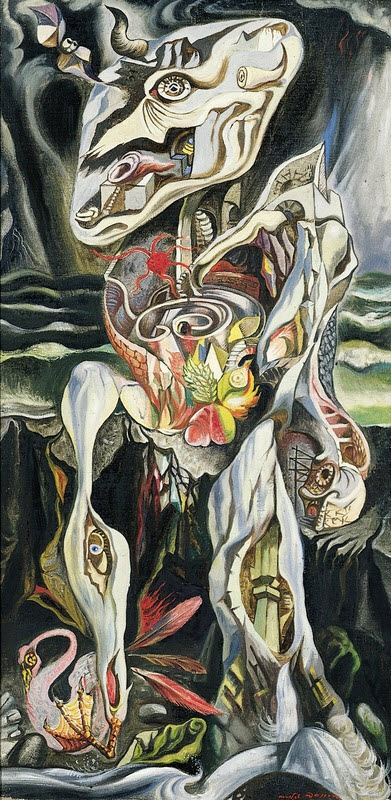
\includegraphics[width=0.75\textwidth]{labyrinthe.jpg}
	\caption{\cite{labyrinthe}}\label{fig:Labyrinthe}
\end{figure}

%Source de la toile : Le Labyrinthe, 1938.- Huile sur toile - 120 x 61 cm - Inscriptions :S.B.DR. : andré Masson- Don Basil et Elisa Goulandris, 1982- Numéro d'inventaire : AM 1982-46 - Centre Pompidou- 

	 Conclure avec cette \oe{}uvre de Masson sur l’espace symbolique réservé à l’homme comme un miroir de lui-même confirme quelle est la finalité des \oe{}uvres de Masson, aussi atypiques les unes des autres soient-elles. On peut ainsi rapprocher ces « miroirs en liberté » des désirs libertaire et de liberté au sens de soulèvement au sein d’une imagerie fantastique qui évoque l’orientation romanesque d’Aragon, notamment depuis 1965 avec \emph{La Mise à mort}. Le miroir du réel bascule chez lui aussi vers une dimension fantastique avec la mise-en-scène obsédante du miroir. 

André Masson révèle cette valeur commune aux deux hommes dans une lettre sur son expérience en Espagne en appelant au lyrisme avec l’imagerie des astres, celle du vertige : 
\begin{quote}
Il y avait un double vertige, l’abîme et le ciel avec les étoiles filantes, le ciel lui-même m’apparaissait comme un abîme, ce que je n’avais jamais ressenti, le vertige du haut en même temps que le vertige du bas. Et je me suis retrouvé dans une espèce de maëlstrom, presque une tempête, et comme hystérique…\footcite{mythologie}\end{quote}
 
	 C’est précisément le mouvement du \enquote{double vertige} qui provoque le basculement vers le fantastique, à l’image du traitement esthétique de Masson des désirs personnels et politiques de ses sujets picturaux. Ce n’est donc pas un hasard si dans un article d’un autre numéro de 1967 en hommage à Miró, le chroniqueur Hubert Juin rassemble le peintre d'André Masson sur un aspect particulier : 
\begin{quote}
Cette liberté devait se payer. Comptant. Il devint beaucoup plus difficile de faire illusion. La peinture était devenue sa propre anecdote. Est-ce à dire qu’elle n’empruntait plus rien au monde extérieur ?  Au contraire. Seule, la servilité était interdite. Son vocabulaire vient de là. Ses racines sont prisonnières de l’épaisseur de la terre, s’y agrippent. Quoi d’autre chez Picasso ? Et chez André Masson, en ceci véritablement exemplaire ? […] Il ne s’agit plus de copier la nature. Il s’agit d’être \emph{comme} la nature. Il s’agit des dire. Il s’agit d’être.\footcite{joanmiro}\end{quote}	 


\begin{figure}[H]
   \centering
   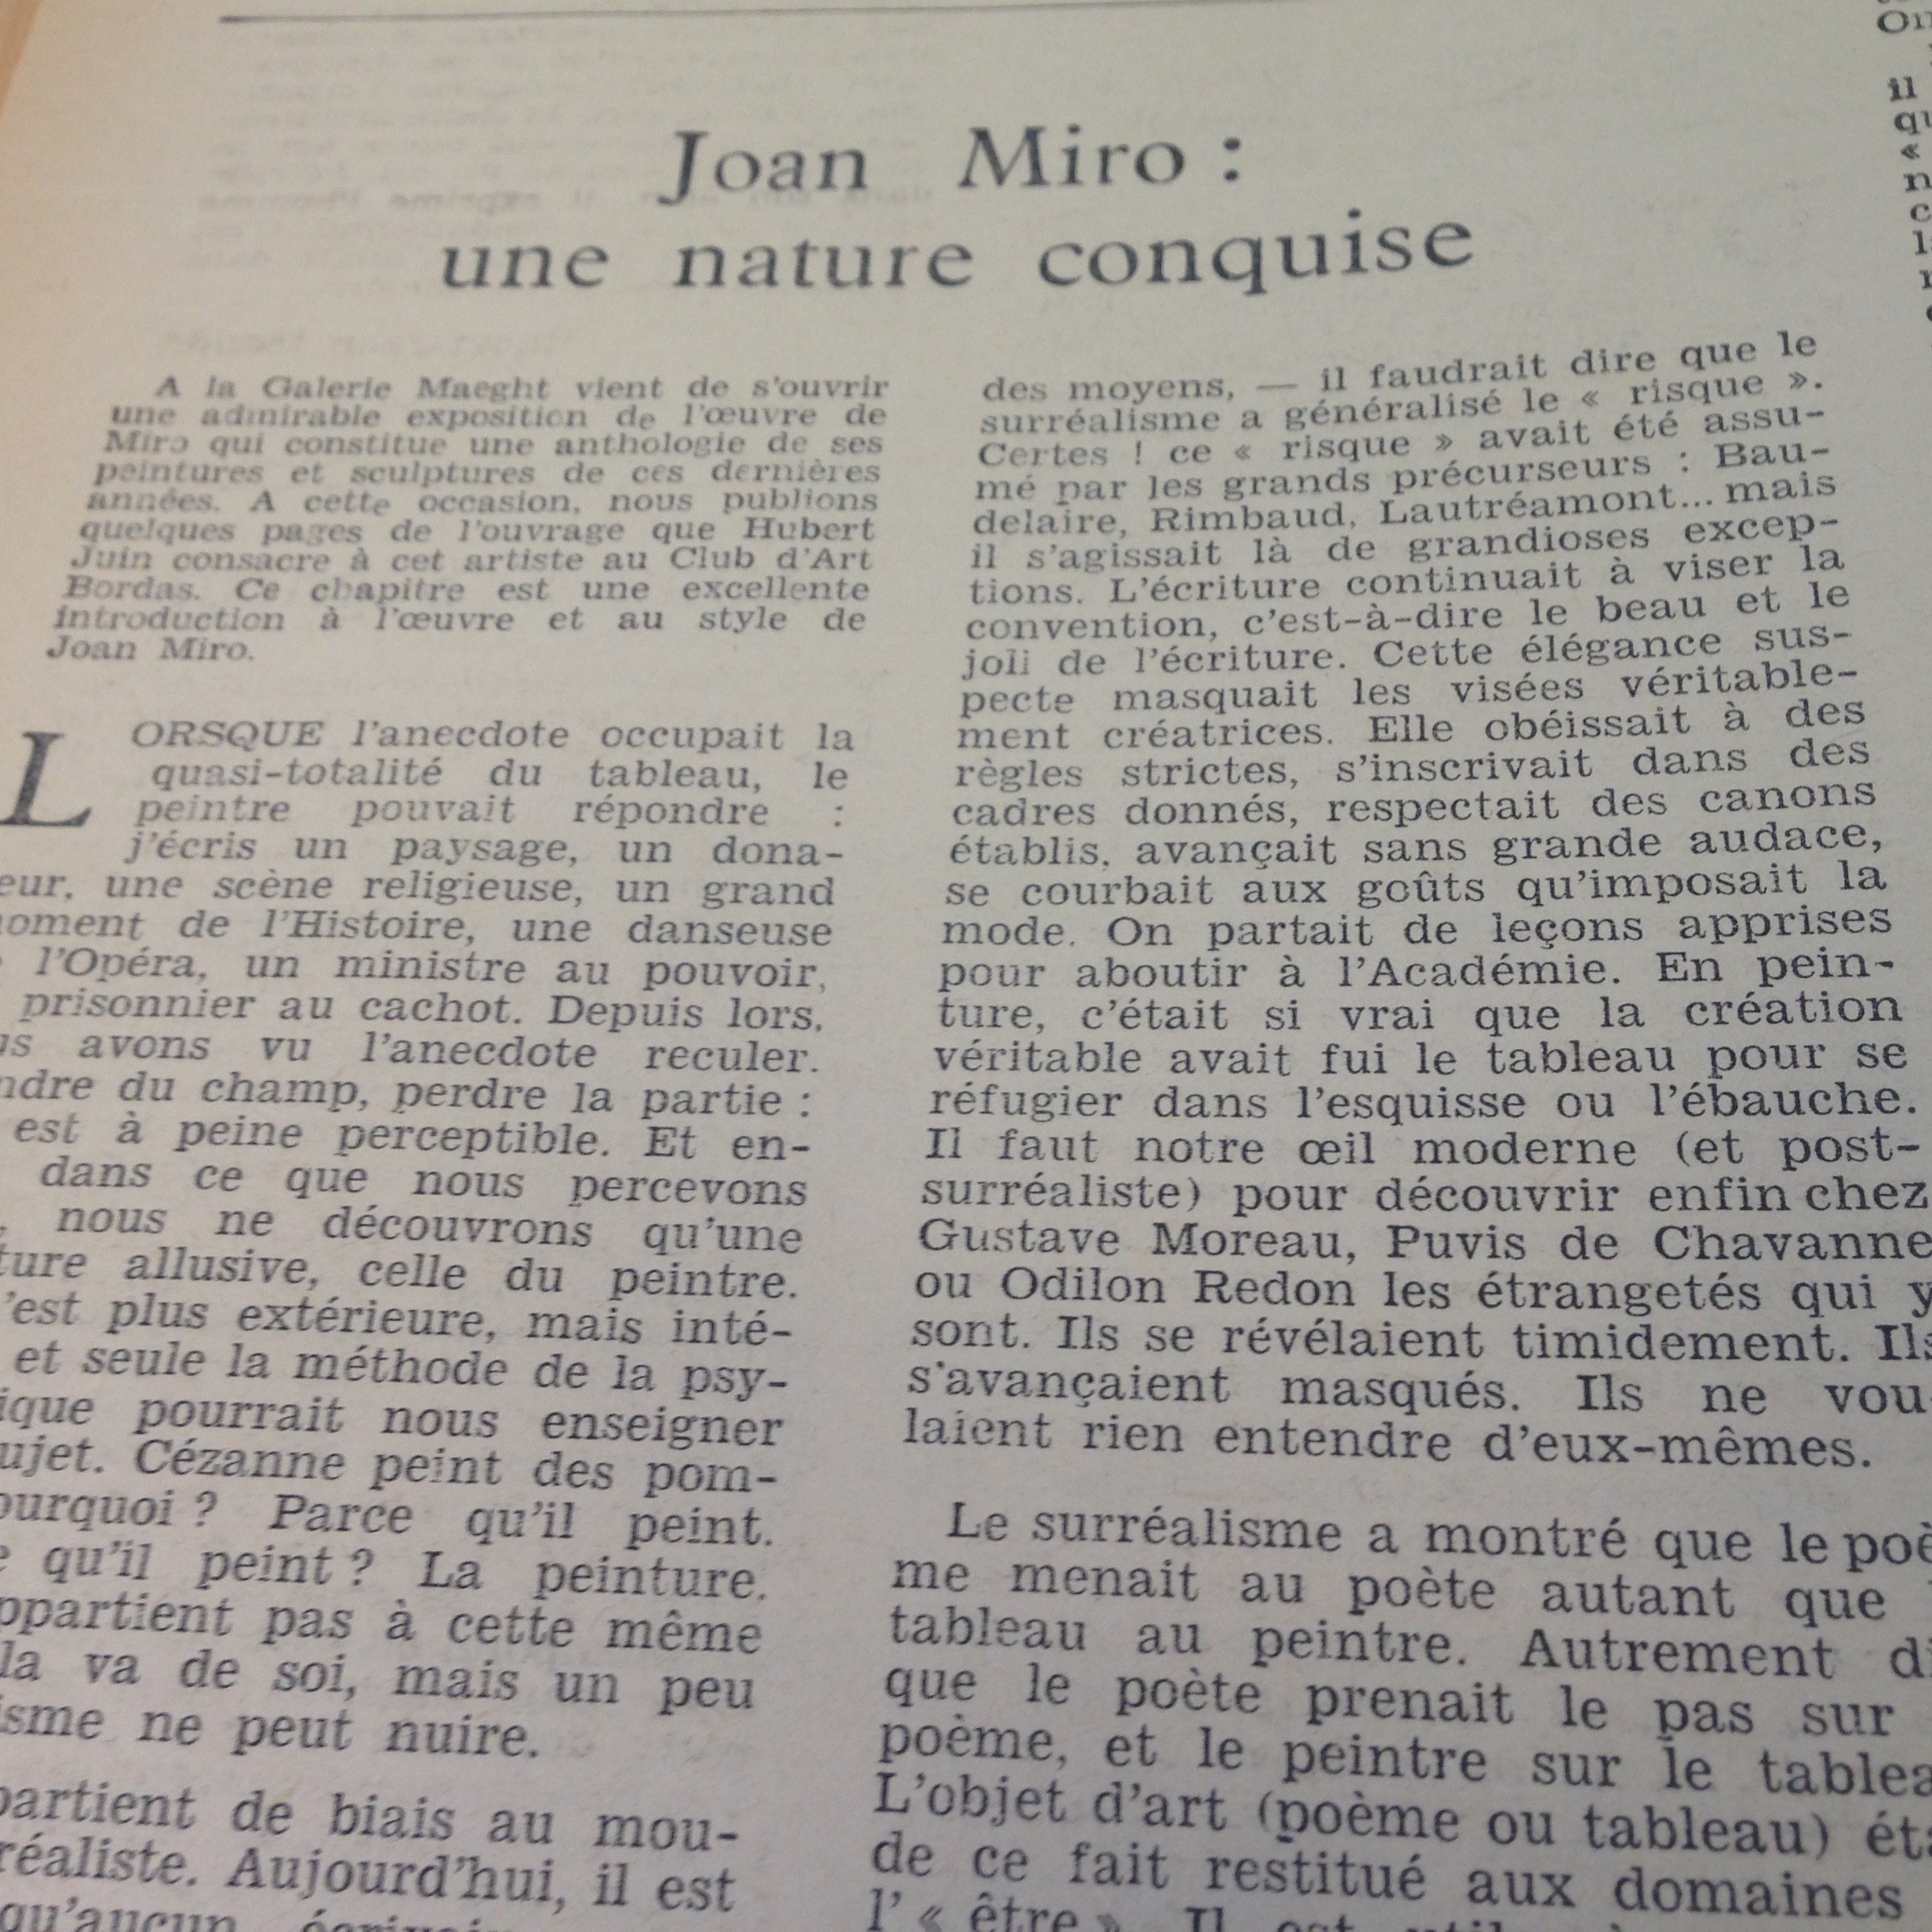
\includegraphics[width=0.75\textwidth]{miron1180.jpg}
	\caption{\cite{joanmiro}}\label{fig:Miro}
\end{figure}

	Ainsi, avec cette recherche esthétique du vertige, André Masson détourne la figuration pour exprimer la nature humaine, et l’on voit  quelle conception politique cette exigence repose, opposée à la \enquote{servilité}. 

	L’exploitation de ces puissants sèmes chez différents chroniqueurs des \emph{Lettres françaises} pour traiter le \enquote{baroquisme tumultueux}d’André Masson peut être aux propres écrits de Masson  pour le journal. Il intervient deux fois selon deux démarches différentes au cours de l’année 1968. En février, Masson écrit parmi d’autres interventions sur sa vision de Baudelaire, bien que la préface des \emph{Lettres françaises} souligne spécifiquement la qualité de l’écrit de Masson en particulier. 

	Plus tôt, en janvier, Masson répond à une enquête sur l’art abstrait, basée à partir d’une citation de Malraux. \emph{Les Lettres françaises} n’en sont pas à leur première enquête, ni Masson à sa première participation : il avait déjà répondu aux côtés d’Elsa Triolet à \emph{Qu’est-ce que l’avant-garde en 1958 ?}. Les deux réponses étaient accolées l'une à l'autre à la Une du numéro.En 1964, \emph{textLes Lettres françaises}publient une immense enquête sur le livre de poche. On peut y retrouver une allusion, comme un clin d’\oe{}il, dans une brève phrase, un paragraphe à elle seule dans \emph{La Mise à mort} un an plus tard.

\subsection{ Exemples d'écrits d'André Masson}

Avec ces deux exemples d’écriture dans \emph{Les Lettres françaises} déjà pratiquées par André Masson, il en appelle en 1953 à sauvegarder la figure de Cézanne (entreprise que le chroniqueur Jean Bouret poursuit en 1965, où Cézanne est oublié dans sa propre région), rend hommage à Turner en 1952. Son intervention dans le journal est le plus souvent destinée à écrire sur une autre figure artistique. Dans le cas de Février 68, Baudelaire se distingue des autres écrits de Masson puisque le sujet n'est pas directement lié à la peinture. Mais c’est par ses écrits sur l’art que Masson établit un premier rapport entre eux. De fait, la préface de George Besson rappelle que c’est au sujet de son travail de critique d’art et son analyse de la modernité que la conférence se tenait : \enquote{Du 8 au 13 janvier, s’est tenu, sous le titre :  “Découverte du présent“ un hommage à Baudelaire, critique d’art que nous avons annoncé en son temps.}\footcite{baudelairepeintres}.

% 2 sources *Cézanne : Les Lettres françaises [n\degre473- 9 au 16 juillet 1953], "Cézanne en visite chez Cézanne" après André Masson. (Fait) / *Turner : Les Lettres françaises [n°398- 24 janvier 1952] 


	 André Masson intervient donc une nouvelle fois en tant qu’artiste, mais aussi avec le recul du commentateur d’art. Ses interventions régulières sur le sujet dans \emph{Les Lettres françaises} nous traduisent un certain plaisir de l’artiste à changer de statut pour celui de l’analyste. Et peut-être plus globalement un plaisir de l’écriture, si l’on tient compte de la prolifération d’écrits épistolaires. En outre, le chroniqueur qui présente les différentes interventions, Georges Besson, critique d’art estimé, est aussi l’un des plus anciens chroniqueurs du journal. Depuis 1958, il tient régulièrement une chronique d’art, \emph{Lettre à une Provinciale}. La figure médiatrice de George Besson est donc particulièrement symbolique du lien de Masson avec le journal,comme fidèle des \emph{Lettres françaises} et ami de Masson :
\begin{quote}
Faute de pouvoir reproduire ici les seize communications qui furent lue et les débats qui s’ensuivirent, nous limitons notre publication à des extraits des textes qui nous semblent les plus significatifs, en donnant la plus large place à l’étude d’André Masson qui éclaire la position de Baudelaire, critique d’art, d’un point de vue personnel et original.\footcite{baudelairepeintres}\end{quote}

	En mettant à l’honneur le texte d’André Masson, \emph{Baudelaire et les peintres}, George Besson souligne l’intérêt d’une inversion de rôle où le peintre écrit sur le critique, mais pas seulement. Une dimension intime est introduite avant même la découverte du texte de Masson. Et, de fait, l’un des éléments chez Baudelaire qui fascine André Masson s’applique dans le contexte à l’écrit sur l’art, mais il serait possible dans les mots du peintre d’en faire un mode de vie : 
\begin{quote}
Il sait que la sagesse serait de ne rien dire de ce qui ne vous dit rien, la nature et les formes de la sympathie jouant totalement de l’appréciation de l’\oe{}uvre d’art, mais parfois il lui faut passer outre et ne pas craindre les dangers de la partialité volontaire jointe à la “force de la contradiction“.\footcite{baudelairepeintres}\end{quote}

Ce commentaire Besson insiste à propos du texte de Masson sur l’aspect \enquote{personnel} et \enquote{original} du texte : dans son texte, André Masson loue une prise de risques de la part de Baudelaire à écrire, y compris quand il n’est pas connaisseur de son sujet. Autrement dit, André Masson préconise cet enthousiasme de l’écrit sur le sujet, au détriment de la dit sagesse. Ne pas craindre l’ignorance. Mais bien plus encore, André Masson fait l’éloge chez Baudelaire d’une écriture subjective, de même qu’il conçoit la réception d’une \oe{}uvre comme étant par essence subjective. Ce \enquote{danger de la partialité volontaire} apparait donc comme étant en réalité une qualité essentielle. Ce qui est déjà un décalage complet vis-à-vis des horizons d’attentes qu’un lecteur aurait envers un critique, et sans doute actuellement encore. 

	D’autant part, non seulement Masson revendique cette subjectivité, tout en ayant conscience d’autres valeurs concernant la précaution minimalisée, mais les risques mêmes que cette subjectivité apportent deviennent des motifs de réussites dans le travail d’écrit sur l’art. Cette \enquote{force de la contradiction} est clairement revendiquée plus que décriée. Ce topos récurrant dans le texte de Masson correspond ainsi avec le discours qu'il tient sur ses propres \oe{}vres.

Cette dualité à laquelle aspire André Masson en l’estimant chez Baudelaire prolonge la manifestation des désirs au sens large, comme il la pratique en tant qu’artiste, et comme elle apparait nécessaire selon lui dans la critique. Cette conception est d’autant plus forte si l’on se réfère à la poésie de Baudelaire :\enquote{Il y a dans tout homme à toute heure deux postulations simultanées, l’invocation vers Dieu ou spiritualité et l’invocation vers Satan ou l’animalité.}Autrement dit, cette expression chez Masson une fois encore récompense le désir. 

	Cet exemple d'écrit de Masson sur Baudelaire correspond avec la dimension de projection caractéristique des \emph{Lettres françaises}.C’est au nom d’une marque d’expression caractéristique chez Masson que celui-ci se projette sur Baudelaire : \enquote{Baudelaire est, profondément, un poète tragique, dénonçant l’ordre factice et l’harmonie conventionnelle. Nul accord parfait, cette âme est pleine de dissonances.} 

Cette notion de \enquote{tragique} que Masson attribue à Baudelaire pour qualifier son art est aussi reprise par Paule Gauthier à son propre sujet dans le titre d’un autre article dans un numéro ultérieur en mai 68, \emph{La sérénité de l’expression tragique d’André Masson}\footcite{expressiontragique}.Au nom de la dimension \enquote{tragique} de sa poésie, et toujours contrairement à un horizon d’attente sur toute \oe{}uvre,l’harmonie n’est pas un idéal. Tout au contraire, dans ce topos musical, elle est mise à mal par la rupture, le désordre. A l’opposé d’une symbiose parfaite, fausse, et surtout sans réflexions. 


	
 Le tragique de Baudelaire comme pour Masson impliquerait donc par essence une révolte, c’est-à-dire l’idée de briser cette convention de l’ordre que dénonce Masson. Une nature politique est ainsi attribuée à l’imitation d’une action noble qu’implique initialement sa définition dans \emph{le Traité de la Poétique} d’Aristote. Or, l’action noble n’est plus le maintien de l’ordre, mais son bouleversement. Par conséquent, parler de Baudelaire dans ce texte suggère la position du spectateur devant un tableau de Masson : 

\begin{quote}
 Les puissances de l’imagination et par conséquent la force de l’image, son irruption dans notre c\oe{}ur et dans notre esprit font partie pour Baudelaire du poète sacré. Pourtant, il n’est d’image que de l’homme. Le peintre-poète obéissant à son intuition lyrique projette dans la nature ses pulsions les plus vives afin qu’elle atteigne à son identification. Les ciels tumultueux, les coups de théâtre de la foudre, la fureur des \enquote{décors} ou \enquote{toiles de fond} mais accompagnements emblématiques de la Passion humaine.\footcite{baudelairepeintres}\end{quote}
 
 Il est intéressant de voir comment Masson détourne la valeur d’abord spirituelle du \enquote{poète sacré}pour au contraire revenir à échelle humaine avec cette vérité générale, et sûrement le fondement de son art : tout ramène à l’homme. 

	L’homme pour Masson, c’est aussi ce à quoi l’homme aspire, cette \enquote{Passion humaine}. Cette finalité, tant artistique que philosophique, est aussi l’homme en tant que tel. On voit le déchainement à travers la propre envolée lyrique de Masson, par successions de métaphores, comment la figure de Baudelaire a éveillé sa propre Passion : ce topos du théâtre n’est pas seulement un imaginaire intime, il est aussi une référence aux projets de Masson avec Jean-Louis Barrault sur les décors et les costumes de pièces, le plafond de l’Odéon, sans compter ses allusions précédentes à la tragédie. Le théâtre va donc de pair avec un autre fameux topos propre au mouvement Romantique pour signifier la Passion autour de la foudre, les métaphores du déchainement météorologique. Les chroniqueurs des \emph{Lettres françaises} évoquent donc l’\oe{}uvre de Masson et ce même discours qui est celui de Masson lui-même pour signifier la Passion humaine. 

Ce parti pris des choses exigé dans les \oe{}uvres d’art et tout sujets, André Masson rattache cette valeur à une certaine tradition philosophique. Kant, dans sa \emph{Critique de la raison pratique}, conçoit la passion comme une entité réflexive, \enquote{La passion se donne le temps et, aussi puissante qu’elle soit, elle réfléchit pour atteindre son but.}. Concept que rejoint André Masson en associant l’acte de la pensée à la pulsion du traitement de ses sujets. Dans son \emph{Traité de la nature humaine}, Hume associe également la passion aux émotions, mais aussi aux idées et à la réflexion : \enquote{Les questions de l'entendement et des passions font à elles seules une suite complète de raisonnements, et j'ai eu envie de tirer parti de cette division naturelle pour tester le goût du public.}\footcite{hume}  Masson reprend ainsi cette notion philosophique au regard de ces penseurs du XVIIIème siècle, avec dans sa propre exigence de peintre et de critique l’entremêlement de la force de l’\oe{}uvre et son lyrisme. 

	 André Masson conclut d’ailleurs sur une anecdote qui révèle dans son passé surréaliste cette perpétuelle volonté de jouer de références pour construire la réflexion du mouvement : \enquote{Je disais un jour à Paul Eluard : “Le père de notre Eglise ce n’est pas Rimbaud, c’est Baudelaire“. J’ajoute qu’il m’approuva sans réserve}. L'usage fréquent chez Masson de ces figures fortes pour incarner le surréalisme s’appuie sur des moments dans l’Histoire qui répondent manifestement à ses propres idéologies. Paradoxalement c’est pour les mêmes raisons qu’Aragon s’attache à la figure de Rimbaud que Masson lui préfère Baudelaire. Un rapport intime pour une figure qui incarnerait la passion, en particulier celle de la révolte. 

	Mais la réelle distinction entre Rimbaud et Baudelaire chez Masson se fait probablement sur l’idée du \enquote{tragique} : Françoise Levaillaint rappelle la nature profondément angoissée d’André Masson, répercutée dans son art et ses relations. En particulier amoureuses, lors de mouvements brusques et parfois violents de son humeur. Bernard Noël montre comment cette angoisse produit le vertige : \enquote{Ce délire aiguillonne le travail Masson et le conduit à l’excès, à la violence, au tragique, non pour les cultiver, mais pour obéir à un emportement profond et naturel}\footcite[p83]{noel}.  Ainsi, de même que ses \oe{}uvres sur l’essence de l’homme, Masson révèle dans son texte sur Baudelaire un nature profondément idéologique qui révèle ses propres traits esthétiques. De même qu’à l’inverse dans son art pictural, l’esthétique mouvementée conduit à son impulsion idéologique. 

C’est un constat analogue que l’on peut tirer de la brève mais efficace réponse de Masson à l’enquête sur l’art abstrait quelques mois plus tôt en Janvier 1968. On peut se demander si cette enquête sur l’art abstrait n’est pas un clin d’\oe{}il à l’enquête sur les avant-gardes (\emph{Qu’est-ce que l’avant-garde en 1958 ?}\footcite{avantgarde}), dix ans auparavant.La réponse d’André Masson à l’époque, un bloc de texte qui occupait la première page du numéro conjointement avec celle d’Elsa Triolet, était déjà claire et non sans ironie sur le terme débattu : \enquote{L’AVANT-GARDE ? Mais elle n’existe pas sans une arrière-garde.} L’enquête de 68 est présentée de façon très écolière par la préface, avec une citation et une réponse dialectique : 

\begin{quote}
Dans une récente interview à l’un de nos confrères, André Malraux a dit : “L’abstraction a a représenté la plus grande liberté possible pour le peintre. Mais c’est une école. Elle cessera comme toutes les écoles“. Voulez-vous répondre aux questions suivantes :  I) - Considérez-vous que l’abstraction soit- ou soit devenue- une école ? Qulle que soit votre réponse, dans quel sens comprenez-vous le mot “école“ ?  II. - Quel a  été dans le passé, quel est aujourd’hui l’apport de l’abstraction à l’art du XXème siècle ? III.-Comment envisagez-vous sa fin ou ses développements éventuels ? Et existe-t-il ,à vos yeux, une forme d’art susceptible de succéder à l’abstraction ou de la remplacer ?\footcite{avantgarde}
\end{quote}
 
	 La réponse concise de Masson, en mauvais élève, tient cette fois en une phrase, aussi synthétique qu’énigmatique, comme le suggèrent les points de suspension : \enquote{Masson dit “On peint pour \enquote{être} même fugacement. C’est de cette leçon que l’école du Pacifique est née…“}. Quand on se remémore plusieurs lettres moqueuses de Masson sur l’art abstrait, comparant régulièrement cette esthétique à un « manuel de géométrie », Masson, grâce à cette allusion, réfute l’art abstrait par l’affirmation. Il le fait en énonçant sa propre conception de la finalité de l’\oe{}uvre (\enquote{on peint pour}). Il en demeure qu'André Masson et ses esquisses opèrent un fil médiateur entre les deux intellectuels. Ses esquisses ne sont pas moins que la trace d'une conviction esthétique profonde commune à Aragon et Malraux dont elles sont le symbole. On retrouve d'ailleurs dans les mots de Malraux sur l'esquisse quelques orientations idéologiques qui ne sont pas sans rappeler le combat de toute une vie de Masson si l'on pouvait lui en attribuer un : 

	 \begin{quote}
	 Non que l’esquisse fût tenue, par avance, pour supérieure à l’\oe{}uvre terminée. Il s’agissait d’esquisses d’une nature particulière, parentes de l’Adoration des mages de Léonard, de certains Rembrandt “inachevés“, de presque tous les Daumiers. On peut douter que les esquisses des portraits de Raphaël aient été de cette nature; l’esquisse d’Ingres pour sa Stratonice est inférieure au tableau de Chantilly; mais ces dernières esquisses, qui sont des préparations, des états du tableau, sont soumises à ses lois. Alors que les esquisses de Rubens ne sont pas seulement des états; alors que celle de la Bataille  de Taillebourg est soumise aux lois de Delacroix, et le tableau achevé, aux lois de la critique et à un accord avec le témoignage de nos sens, au traditionnel illusionnisme que Delacroix, dans son Journal, n’ose pas récuser tout à fait. […] L’art entre en conflit avec le “fini“, avec le témoignage de nos sens, avec la peinture en tant que représentation des spectacles.\footcite[p56]{museeimaginaire}\end{quote}

	Ce rapport de force entre l'esquisse et la toile est décrite par Malraux avec le topos de la soumission. Cette notion, que l'on imagine avant tout politique, incarne d'une manière générale le constant refus d'André Masson de céder à cette même soumission. Tout son art, sans compter sa sensibilité politique, est dirigé contre lui. Comme le manifeste ses notes dans sa \emph{Mémoire du Monde} sur ses fugues sur le champ de bataille, et les tentatives d'échapper aux hopitaux psychiatriques. Sans oublier certains doutes sur les thèses marxistes précédemment évoquées.
	
	\subsection{André Masson : passerelle entre Aragon et André Malraux }
	 Le parti pris de l'esquisse chez Masson, le goût prononcé du trait, pourrait s'expliquer en partie par l'idée de prendre position dans cette dualité énoncée par Malraux pour l'inachevé, qui comporte chez Masson probablement une part d'inssaisissable, une prise de liberté du trait par l'esquisse. De même que l'obsession du thème de la métamorphose est un signe récurrent chez Masson, liées à leurs précédentes collaborations autout de l'érotisme. Le thème de la métamorphose lie également les créations de Masson et un projet tel que celui du \emph{Musée imaginaire} :\enquote{Le Musée imaginaire naît d’une métamorphose aussi profonde que celle dont naquirent les premières collections italiennes : comme les dieux antiques lors de la Renaissance, les dieux qui ressuscitent devant nous sont amputés de leur divinité}\footcite[p179]{museeimaginaire}. Une telle définition peut se confondre avec le projet visuel de Masson qui fait de la métamorphose une autre réalité, le revers du visible.  Cette spéficité propre de la métamorphose  chez Masson et la sensiblité à l'esquisse le désigne comme figure médiatrice entre Aragon et Malraux. 
	

	L'exemple de la collaboration entre Aragon et André Masson Pablo Neruda en décembre 1965 a l'avantage d'éclairer sur ces rapprochements connus mais moins marqués dans les mémoires que ceux de la période surréaliste qui a pourtant tout autant dans une autre mesure marquée les esprits de personnalités autant impliquées dans le conflit de la guerre civile d'Espagne que ne l'auront été André Masson, Aragon, et André Malraux. L'engagement de Masson et Aragon particulièrement manifeste un rapprochement idéologique quelques années après les distinctions de prises de positions vis-à-vis du parti communsite, et possiblement un deuxième temps d'amitié entre les deux hommes auquel ce numéro de décembre 1965 rend aussi hommage. 
	

Mais il faudrait à la fois comparer la proximité esthétique chez Aragon et chez Masson pour l'esquisse et ce parti pris des \emph{Lettres françaises} réservé spécifiquement à André Masson et les propos d'Aragon et de Malraux sur le sujet la même année en 1947.

Aragon, depuis sa préface aux \emph{Dessins de Fougeron} en 1947 jusqu'en décembre 1965 évolue vis-à-vis de sa ligne politique et esthétique. Pour autant, celle-ci demeure pas moins obsédante et essentielle à ses yeux. Avec Malraux d'autre part, qui écrit la même année \emph{Les voix du silence}, dont l'\oe{}uvre inscrite dans le projet du \emph{Musée imaginaire} est rééditée cette même année de 1965. Le développement qu'y consacre Malraux au sujet de l'esquisse n'est pas sans rappeler et même rejoindre quelques convictions esthétiques et idéologiques d'André Masson. Les deux hommes sont d'ailleurs amis et ont collaboré ensemble sur une \oe{}uvre telle que \emph{Les conquérants} en 1929. André Masson agirait ainsi comme une figure médiatrice entre ces deux intellectuels, mais dont l'on retrouve dans les lignes de Malraux une vision commune sur l'esquisse et ce qu'elle implique, à commencer en matière d'esthétique : 

\begin{quote}
 L’esquisse est, en principe, un “état“ de l’\oe{}uvre antérieur à son achèvement, à l’exécution de ses détails surtout. Mais il en existe un type particulier : cela où le peintre, ne tenant pas compte du spectateur et indifférent à l’illusion, a réduit un spectacle réel ou imaginaire à ce par quoi il devient peinture : taches, couleurs, mouvements.\footcite[p52]{museeimaginaire}\end{quote} 

Malraux conçoit ainsi l'art de l'esquisse comme l'étape du détail par excellence, ce qui peut paraitre au premier abord paradoxal avec sa nature inachvée qu'il lui reconnaît tout autant. Tout comme Aragon dans sa préface aux \emph{Dessins de Fougeron}, l'esquisse n'est plus une étape ni même un enjeu vis-à-vis de la peinture, elle est son processus :

\begin{quote}
Et l’on vit le maître épouvanté de sa maîtrise imiter à grand peine la maladresse de l’élève, le tremblant devenant le témoin de l’émotion sacrée, l’accident l’essentiel, l’inachevé seule satisfaction. […]C’est peut-être pourquoi je me méfie des peintres dont on ne voit jamais les dessins. Que me cachent-ils ? Pourquoi ne veulent-ils pas que je voie le squelette de leur pensée ?\footcite[p133]{ecritssurla}\end{quote} 

Il est intéressant que ce que Malraux décrit comme un \enquote{état} marquée par le détail, pour ne pas dire le moment où l'artiste révèle sa spécificité, Aragon en vient à la même conclusion avec un registre plus lyrique, expliqué en partie du fait que la marque de l'artiste ne vient pas de sa rigueur mais de, \enquote{la maladresse}, \enquote{l'émotion sacrée}, \enquote{l'accident} dont ces aspects semblent se résumer dans la notion d'\enquote{inachevé}. Masson incarne ainsi avec sa recherche de \enquote{l'illimité} la frontière entre le vertige argonien et la métamorphose du musée imaginaire, ce double projet entre Masson et Malraux de métamorphose de l'\oe{}uvre mais aussi la \enquote{métamorpose du regard} : 

\begin{quote}
« Il va de soi que l’immense métamorphose qui avait fait, de la volonté d’exprimer le surnaturel, une maladroite intention d’imiter la nature - instituant celle-ci juge du surnaturel, et effaçant ainsi un millénaire d’art chrétien - était inséparable d’une métamorphose du regard. La création de tout grand art est inséparable d’une telle métamorphose, qui n’appartient point au domaine de la vision, mais de l’attentionnée et d’une sorte de projection sur l’\oe{}uvre, qui mène le spectateur à y reconnaître ce qu’il en attend, fétiche ou statue.\footcite{p201}\end{quote}

L'appréhension d'un nouveau regard sur l'\oe{}uvre est intimement liée à l'utopie chère à Masson et Malraux de quitter la référence à la nature, pour tendre chez Malraux vers le sacré, ce qui n'est pas si éloigné de l'expression \enquote{fête pour les yeux} chère à Masson empruntée dans le journal de Delacroix. 

	 Et peut-être Pablo Neruda est-il une autre de ces présences médiatrices entre Aragon et Masson, pour cette sensibilité et ce combat commun pendant la guerre d'Espagne, l'événement symboliquement enfoui derrière celui du tremblement de terre du Chili qui fait perdre à Neruda sa maison auquel leur collaboration est dédiée. 

	Cette question de l'esquisse en 1965 où Masson figurerait la passerelle entre Aragon et Malraux illsutre aussi l'évolution de la perspective politique abordée dans \emph{Les Lettres françaises} dans les années 1960, toujours aussi ancrée dans ce journal culturel, mais reconsidérée sans le réalisme socialiste qui influençait son discours dans son texte dédié aux \emph{Dessins de Fougeron}. Cette évolution est relatée par Philippe Olivera dans son article centre sur les années de 1958 à 1968 du journal : 


	\begin{quote}
		
	\end{quote}



Ainsi, le geste du dessin qui jouait un rôle fondateur dans le texte d'Aragon sur les dessins de Fougeron évolue même après le déclin du réalisme sociliste. Et peut-être son rapprochement idélogique notamment au sein du journal avec André Masson comme le symbolise leur collaboration autour de la figure de Neruda illustre aussi l'évolution de sa formule, \enquote{ Oui, c’est le destin de l’art figuratif qui se joue à chaque dessin.}\footcite[p135]{ecritssurla} Toujours est-il que cette conviction de favoriser le dessin à la toile, l'inachevé à l'achevé, reste une profonde conviction communiste chez Aragon mais qui remonte déjà au moins jusqu'à la période de la jeunesse surréaliste chez Masson comme chez Aragon, pour finir par être l'un des motifs de rassemblement entre les deux hommes dans ces années 1960 parmi les jeux d'échos de leurs correspondances opérées par \emph{Les Lettres françaises}

	Or, c’est justement l’absence de finalité qui provoque dans ses correspondances le scepticisme de Masson pour l’abstrait, avec ce topos  de la géométrie. L’adverbe \enquote{fugacement} pourrait toutefois évoquer le mouvement vif du trait qui jaillit propre à l’esthétique abstraite. Si ce n’est qu’elle est surtout caractéristique sous la plume de Masson comme d’un mode de figuration pour incarner l’homme. 

	La référence avec l’Ecole du Pacifique au Nouveau Réalisme, né seulement quelques années auparavant, est un mouvement qui revendique d’exister par sa singularité. L’allusion au Nouveau Réalisme comporte à la fois l’héritage de Dada, dans un journal qui cite Tristan Tzara régulièrement et le mouvement régulièrement, et la vocation d’une nouvelle composition du réel explique amplement l’empathie de Masson pour ce mouvement en pleine expansion. C’est donc à plusieurs échelles que Masson intervient et que son \oe{}uvre se manifeste l’année 1968. Il est intéressant de constater qu’il occupe une place de plus grande ampleur encore que les années précédentes en cette année aussi riche d’événements politiques. Comme \emph{Les Lettres françaises} vont convoquer naturellement Courbet pour parler de la Commune, l’\oe{}uvre d’André Masson et ses interventions occupent régulièrement les numéros dans ces mois de tension politique. 

	Enfin, avec ce jeu de chassé-croisé des écrits respectifs d’André Masson et d’Aragon dans \emph{Les Lettres françaises}, leur collaboration affichée confirme quelle visée esthético-idéologique poursuivent les deux hommes avec des processus distincts.

\section{La collaboration d’Aragon et Masson dans le journal, réactualisation sentimentale et politique d’engagements historiques communs}

La collaboration entre André Masson et Aragon en décembre 65 est hautement symbolique autant par la forme que par le sujet : Aragon intervient non en tant que critique mais en tant que poète, Masson comme dessinateur, avec l’une de ses esquisses comme aiment à les utiliser \emph{Les Lettres françaises}. Et, plus précisément, la légende de l’esquisse de Masson présente ces vers d’Aragon comme\enquote{première étude}.\footcite{pabloneruda}

	 Le propos ensuite autour de la figure de Pablo Neruda incarne un événement politique et historique notable mais vécu intimement par les deux hommes. Tous deux ont pris part à la guerre civile de 1936 du côté des républicains. André Masson vivait avec sa famille en Espagne. Aragon rencontre Pablo Neruda pendant la guerre civile en 1937. Ces aspects montrent bien quelle dimension personnelle avait pris cette bataille politique de défense idéologique. Or, au c\oe{}ur de ce combat politique, c’est par la voie intellectuelle et politique que la rencontre se produit, d’après l’article de Laetitia Boussard sur la relation entre Aragon et Pablo Neruda :


\begin{quote}
Leur rencontre a lieu en France, à Paris, en 1937, dans le contexte de la guerre civile espagnole. Ils font partie du groupe d’intellectuels, lisons-nous dans Confieso que he vivido, qui prépare un congrès devant se dérouler à Madrid et qui réunirait des écrivains anti-fascistes du monde entier. Louis Aragon offre d’ailleurs à Neruda un emploi dans son association, l’aidant ainsi à subvenir à ses besoins. Tous deux s’engagent dans la lutte antifranquiste, Louis Aragon en convoyant des dons de l’association internationale des écrivains pour la défense de la culture, Pablo Neruda en préparant le départ de républicains espagnols pour le Chili à bord du Winnipeg en 1939. Ils se rencontrent dans un contexte historique particulier qui les réunit dans leur lutte contre le fascisme et qui donne naissance chez le poète chilien à España en el corazón, recueil de poèmes publié en 1937 au Chili, puis en France en 1938, préfacé par Louis Aragon. España en el corazón deviendra en 1948 le titre d’un poème dans le \emph{Nouveau Crève-Cœur}.\footcite{aragonaneruda}\end{quote}	 

L’histoire même de leur rencontre, et les prolongements de contact tant \enquote{transtextuels} que sociaux qui ont perduré, implique Pablo Neruda dans cette affirmation chère à Aragon de fixer son identité politique à partir de sa pensée poétique. Leur rencontre est le symbole de cette conception aragonienne. En outre, la légende du dessin d’André Masson rappelle un autre événement arrivé à Pablo Neruda en 1965, le \enquote{tremblement de Terre du Chili au début de cette année où la maison du poète a été détruite}\footcite{pabloneruda}. En somme, Pablo Neruda est présenté par cet événement comme un poète nomade. Il est intéressant que le tremblement de terre et ses conséquences ait inspiré la création d’Aragon comme celle d’André Masson. Ce dernier, comme nous l’avons vu dans d’autres esquisses, mais aussi dans les métaphores astrales de ses écrits, est particulièrement attiré par le processus d’explosion et de jaillissement, autant dans le processus de création que dans la réception de l’\oe{}uvre qui doit se vivre comme une révélation. L’\oe{}uvre poétique de Pablo Neruda aspire à la même forme d’expressivité que les dessins d’André Masson :

\begin{quote}
Le poète au contraire, met par nature au pluriel, il salue avec amour l’infinie multiplicité de l’Etre, il vitrer il nourrit sa pensée et son chant, d’un échange généreux et perpétuel : “Je est un autre“, dit-il sans cesse avec Rimbaud. Aussi “le culte des images“ est-il chez lui non une fuite devant le monde, mais l’affirmation la plus haute du lien qui unit l’homme et le monde, et comme l’annonce faite à l’homme de son pouvoir possible sur le monde.\footcite{marcenac2004pablo}\end{quote}	


	Les deux hommes partagent la conviction puissante d’un réel qui ne peut pas être la reproduction de la Nature. Cette orientation est liée à une idée commune chez Neruda, Masson, et Aragon particulièrement en cette année 1965 riche d’allusion dans \emph{Les Lettres françaises} à \emph{La Mise à mort}, d’une identité altérée, multiple, et en partie irrationnelle. Comme pour l’\oe{}uvre de Masson, celle de Neruda comporte dans cette idée de l’homme une dimension de transformation du monde. Ainsi, l’élan et le mouvement sont au c\oe{}ur de leur imaginaire. Or, c’est peut-être parce que les recherches d’Aragon et André Masson n’ont jamais été aussi proches dans leurs \oe{}uvres respectives qu’en 1965. Tous deux collaborent à cet hommage à Pablo Neruda, et pas seulement en raison d'un riche passé politique commun pendant la guerre civile d’Espagne en 36.  Toujours est-il que le dessin d’André Masson, s’il fait référence à l’événement précis du tremblement de terre, cherche à faire image exactement de la même façon qu’Aragon et son poème \emph{Le Paresseux} reproduit dans cet article. C’est d’ailleurs suite à l’événement de la perte de la maison de Neruda suite au tremblement de terre dans le Chili qu’Aragon publie le recueil \emph{Elégie à Pablo Neruda} dont est extrait ce poème. 

Croiser la réception d’Aragon avec \emph{Le Paresseux} et l’esquisse d’André Masson montre la perception romantique des deux hommes ont de cette catastrophe naturelle. Romantique, parce que c’est une image spécifique du poète qui en résulte : « Continueront voyager choses / de métal entre les étoiles ». Ainsi commence \emph{Le Paresseux}, et cette image lyrique des morceaux de métal au milieu des astres substitue à la tragédie tellurique une dimension poétique. Cette fameuse métaphore astrale si chère à André Masson, notamment pour évoquer ses \oe{}uvres, est traduite dans son dessin minimaliste, fait de petits personnages et de traits vifs, par la figuration d’une étoile sur la partie centrale du haut du dessin, au sommet du croisement des lignes. Comme souvent dans les dessins de Masson, celui-ci paraît rechercher la simplicité maximale, tout en demeurant une énigme. Tout au moins, pas immédiatement compréhensible au premier regard. 

\begin{figure}[H]
   \centering
   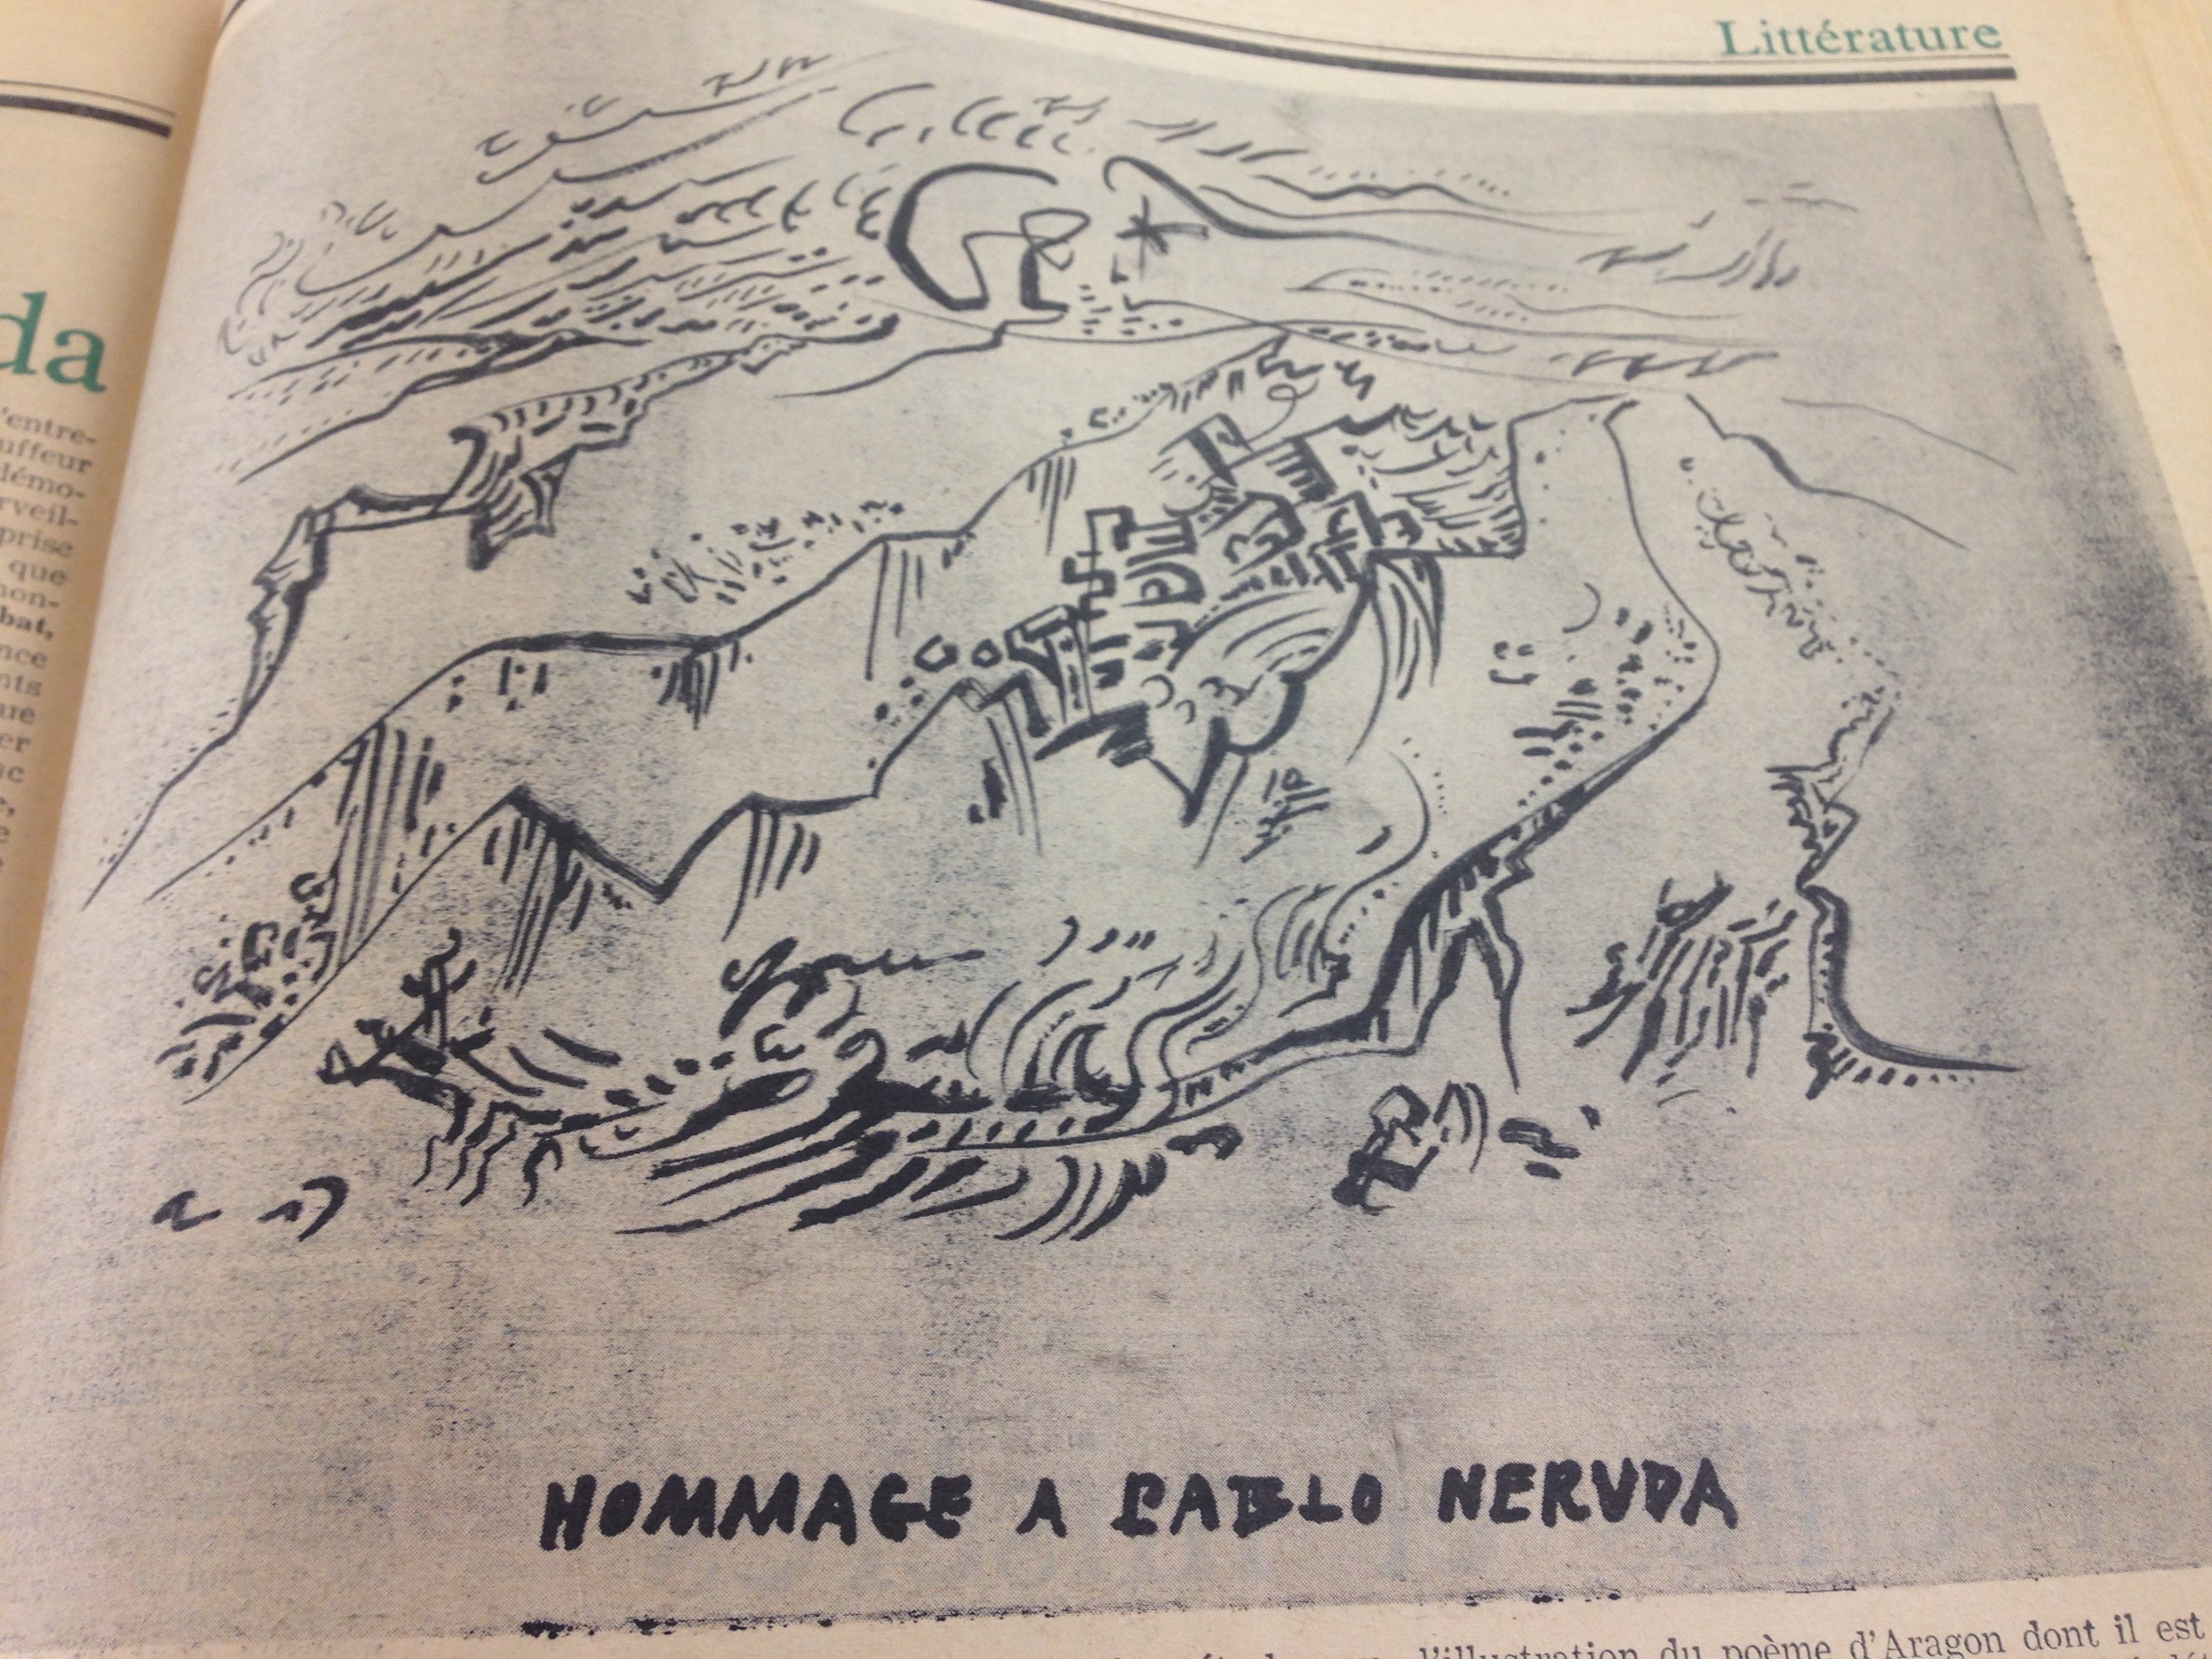
\includegraphics[width=0.75\textwidth]{esquissen1108.jpg}
	\caption{\cite{pabloneruda}}\label{fig:MassonNeruda}
\end{figure}

	Cette esquisse-ci paraît vaste comme dans un plan d’ensemble, avec de longs traits étendus et écartés les uns des autres. Les traits du premier plan, les plus épais, verticaux et parallèles les uns aux autres se rejoignent vers le centre-haut du dessin pour former ce qui se rapprocherait d’un triangle : c’est donc d’abord une montagne que les lignes auraient pour évocation en premier lieu, mais pas seulement. A observer l’esquisse en détail, certaines de ces lignes verticales et courbées forment dans leur élan parallèle la forme d’un oiseau. 

En outre, l’esquisse est riche de petits personnages, sous une forme minimaliste, certains mêmes entre la figuration et le trait pur. Le plus visible d’entre eux se situe au sommet de l’esquisse, les bras faits de petits et fins traits en direction de l’étoile. Or, si la jambe droite du personnage prend appui sur le trait de la montagne, sa jambe gauche est une courbe épaisse autour de son corps, d’une forme similaire à la lune. Ce personnage en hauteur dans les astres au corps composé en partie d’un astre lunaire aux côtés de l’étoile rappelle dans l’imaginaire de Masson la figure du poète. Ainsi, Aragon et Masson dans cette collaboration entremêlent à la fois l’hommage au Chili et au poète qu’est Neruda, avec un même élan lyrique vers une dimension onirique. Par ailleurs, cette représentation commune chez Aragon et Masson rejoint celle argumentée par Jean Marcenac dans son étude :

\begin{quote}
Neruda est ainsi parmi nous un homme qui rattache l’homme à la fois aux autres hommes et au monde. Et c’est parce que le lien qu’il noue est ainsi double qu’il est si puissant, indissoluble. L’apport immense de Neruda, dans la poésie d’aujourd’hui se ramène à cette affirmation jumelle : qu’il n’est de poésie que de l’homme - ce que nous savions - et qu’il n’est d’homme que de la terre - ce que peut-être un certain \enquote{humanisme} nous avait fait oublier.\footcite[p119]{pabloneruda}\end{quote}

Cette notion de terre, tout comme la lumière, constitue d’ailleurs les grands thèmes de la poésie de Neruda. C’est également cette double filiation décrite par Marcenac que révèlent Aragon par le biais de l’imagerie poétique, Masson par le dessin. Ainsi, le Chili évoque simultanément la terre du poète et le poète lui-même : \enquote{Au Chili les cerises dansent, / les obscures jeunes filles chantent, / et l'eau brille sur les guitares.}\footcite{pabloneruda} Dans cette troisième strophe du Paresseux, le poète Aragon voit la terre chilienne avec les yeux de Neruda lui-même, et c’est ce lyrisme qui le pousse à cette affirmation au vers final : \enquote{Je ne veux pas changer de planète}\footcite{pabloneruda}.  On ne peut exclure une certaine forme de résistance chez le poète accompagné par un lyrisme des terres chiliennes : \emph{Le Paresseux }ne part pas après le tremblement de terre, il se sent encore rattaché à cette terre chilienne. L’esquisse d’André Masson rejoint cette image du poète littéralement composé du monde, avec ce petit pzrsonnage fait en partie d’astres et donc le corps composé de lignes se mêle à celles du tremblement de terre. Ces lignes courbes verticales à la formes triangulaires proches de la montagne. Tous les personnes qui gravitent autour du tremblement, et parfois entraperçus par des fragments de corps à l’intérieur même du tremblement de terre en train de jaillir dans l’élan vif des lignes, sont en réalité des compositions du tremblement de terre en train de jaillir. 

	En outre, la figure confondue, dans \emph{Le Paresseux}, de la terre et du poète évoque d’une part le souci de transtextualité cher à Aragon, à savoir mêler à ses vers ceux de Pablo Neruda. C’est pourquoi, à la fin de son recueil \emph{Le Nouveau Crève-C\oe{}ur}, Aragon mêlait déjà ces deux figures, à tel point que la relecture de ces poèmes en hommage à Neruda révèle des figures qui semblent annoncer le terrible événement, bien que ce soit le topos du feu qui soit le plus récemment associé au poète Neruda : 

\begin{verse}
A Madrid il est consul 
En trente-six quand le feu
Change sur la péninsule
En ciel rouge le ciel bleu\footcite{pabloneruda}	
\end{verse}
 
	La scène décrite est ambiguë : la description annoncerait un contexte apocalyptique, digne du réel tremblement de terre dévastateur quelques années plus tard, et pourtant c’est aussi exactement le contraire que sous-entendent les références absolues et la figure d’autorité de \enquote{consul}attribuée à Neruda. Et peut-être aussi l’affection manifestée par Aragon dans cette \emph{Complainte à Pablo Neruda} qui rend plus plausible l’hypothèse d’un changement positif attribué à Neruda du changement de l’atmosphère politique en Espagne. Aragon va jusqu'à faire de Neruda la figure d’autorité qui aurait commandité la transition insurrectionnelle de trente-six depuis la proclamation de la 1ère République du 14 avril 1936. Le feu a priori dévastateur est aussi la force tant poétique qu’insurrectionnelle du poète Neruda avide de liberté. Or, c’est aussi cette même liberté qu’Aragon prête à la maison du poète, associée à la figure féminine. C’est même cette tournure lyrique finale qui convoque l’image de la figure féminine mais aussi comme la \emph{Passante} de Baudelaire, c'est-à-dire comme la liberté en sens le plus large. Devant cet entremêlement de la Beauté incarnée par la femme et de la liberté, à l’image des éléments naturels tels que le tremblement de terre qui emporte la maison, le lyrisme de l’atmosphère suffit à justifier l’affirmation en strophe finale : \enquote{Je ne veux pas changer de planète.}\footcite{pabloneruda}

Ainsi, André Masson et Pablo Neruda partagent cette fascination essentielle dans leur \oe{}uvre une image du mouvement pris sur le vif, dans le jaillissement de l’expression en train de devenir. En somme, le poème \emph{Le Paresseux} d’Aragon comme l’esquisse de Masson s’attachent non au tremblement en tant que catastrophe, mais comme portrait lyrique du poète Neruda, et des hommes en général comme ses propres poèmes s’y vouent : l’identité inconsistante et en perpétuelle composition de l’homme.

